\documentclass[]{elsarticle} %review=doublespace preprint=single 5p=2 column
%%% Begin My package additions %%%%%%%%%%%%%%%%%%%
\usepackage[hyphens]{url}

  \journal{WG-EMM 2021} % Sets Journal name


\usepackage{lineno} % add
\providecommand{\tightlist}{%
  \setlength{\itemsep}{0pt}\setlength{\parskip}{0pt}}

\usepackage{graphicx}
\usepackage{booktabs} % book-quality tables
%%%%%%%%%%%%%%%% end my additions to header

\usepackage[T1]{fontenc}
\usepackage{lmodern}
\usepackage{amssymb,amsmath}
\usepackage{ifxetex,ifluatex}
\usepackage{fixltx2e} % provides \textsubscript
% use upquote if available, for straight quotes in verbatim environments
\IfFileExists{upquote.sty}{\usepackage{upquote}}{}
\ifnum 0\ifxetex 1\fi\ifluatex 1\fi=0 % if pdftex
  \usepackage[utf8]{inputenc}
\else % if luatex or xelatex
  \usepackage{fontspec}
  \ifxetex
    \usepackage{xltxtra,xunicode}
  \fi
  \defaultfontfeatures{Mapping=tex-text,Scale=MatchLowercase}
  \newcommand{\euro}{€}
\fi
% use microtype if available
\IfFileExists{microtype.sty}{\usepackage{microtype}}{}
\usepackage[margin=3cm]{geometry}
\bibliographystyle{elsarticle-harv}
\usepackage{color}
\usepackage{fancyvrb}
\newcommand{\VerbBar}{|}
\newcommand{\VERB}{\Verb[commandchars=\\\{\}]}
\DefineVerbatimEnvironment{Highlighting}{Verbatim}{commandchars=\\\{\}}
% Add ',fontsize=\small' for more characters per line
\usepackage{framed}
\definecolor{shadecolor}{RGB}{248,248,248}
\newenvironment{Shaded}{\begin{snugshade}}{\end{snugshade}}
\newcommand{\AlertTok}[1]{\textcolor[rgb]{0.94,0.16,0.16}{#1}}
\newcommand{\AnnotationTok}[1]{\textcolor[rgb]{0.56,0.35,0.01}{\textbf{\textit{#1}}}}
\newcommand{\AttributeTok}[1]{\textcolor[rgb]{0.77,0.63,0.00}{#1}}
\newcommand{\BaseNTok}[1]{\textcolor[rgb]{0.00,0.00,0.81}{#1}}
\newcommand{\BuiltInTok}[1]{#1}
\newcommand{\CharTok}[1]{\textcolor[rgb]{0.31,0.60,0.02}{#1}}
\newcommand{\CommentTok}[1]{\textcolor[rgb]{0.56,0.35,0.01}{\textit{#1}}}
\newcommand{\CommentVarTok}[1]{\textcolor[rgb]{0.56,0.35,0.01}{\textbf{\textit{#1}}}}
\newcommand{\ConstantTok}[1]{\textcolor[rgb]{0.00,0.00,0.00}{#1}}
\newcommand{\ControlFlowTok}[1]{\textcolor[rgb]{0.13,0.29,0.53}{\textbf{#1}}}
\newcommand{\DataTypeTok}[1]{\textcolor[rgb]{0.13,0.29,0.53}{#1}}
\newcommand{\DecValTok}[1]{\textcolor[rgb]{0.00,0.00,0.81}{#1}}
\newcommand{\DocumentationTok}[1]{\textcolor[rgb]{0.56,0.35,0.01}{\textbf{\textit{#1}}}}
\newcommand{\ErrorTok}[1]{\textcolor[rgb]{0.64,0.00,0.00}{\textbf{#1}}}
\newcommand{\ExtensionTok}[1]{#1}
\newcommand{\FloatTok}[1]{\textcolor[rgb]{0.00,0.00,0.81}{#1}}
\newcommand{\FunctionTok}[1]{\textcolor[rgb]{0.00,0.00,0.00}{#1}}
\newcommand{\ImportTok}[1]{#1}
\newcommand{\InformationTok}[1]{\textcolor[rgb]{0.56,0.35,0.01}{\textbf{\textit{#1}}}}
\newcommand{\KeywordTok}[1]{\textcolor[rgb]{0.13,0.29,0.53}{\textbf{#1}}}
\newcommand{\NormalTok}[1]{#1}
\newcommand{\OperatorTok}[1]{\textcolor[rgb]{0.81,0.36,0.00}{\textbf{#1}}}
\newcommand{\OtherTok}[1]{\textcolor[rgb]{0.56,0.35,0.01}{#1}}
\newcommand{\PreprocessorTok}[1]{\textcolor[rgb]{0.56,0.35,0.01}{\textit{#1}}}
\newcommand{\RegionMarkerTok}[1]{#1}
\newcommand{\SpecialCharTok}[1]{\textcolor[rgb]{0.00,0.00,0.00}{#1}}
\newcommand{\SpecialStringTok}[1]{\textcolor[rgb]{0.31,0.60,0.02}{#1}}
\newcommand{\StringTok}[1]{\textcolor[rgb]{0.31,0.60,0.02}{#1}}
\newcommand{\VariableTok}[1]{\textcolor[rgb]{0.00,0.00,0.00}{#1}}
\newcommand{\VerbatimStringTok}[1]{\textcolor[rgb]{0.31,0.60,0.02}{#1}}
\newcommand{\WarningTok}[1]{\textcolor[rgb]{0.56,0.35,0.01}{\textbf{\textit{#1}}}}
\usepackage{graphicx}
\ifxetex
  \usepackage[setpagesize=false, % page size defined by xetex
              unicode=false, % unicode breaks when used with xetex
              xetex]{hyperref}
\else
  \usepackage[unicode=true]{hyperref}
\fi
\hypersetup{breaklinks=true,
            bookmarks=true,
            pdfauthor={},
            pdftitle={A preliminary evaluation of the evidence supporting fishery-driven localised depletion effects on the performance and demographic trends of pygoscelid penguins in Subarea 48.1},
            colorlinks=false,
            urlcolor=blue,
            linkcolor=magenta,
            pdfborder={0 0 0}}
\urlstyle{same}  % don't use monospace font for urls

\setcounter{secnumdepth}{0}
% Pandoc toggle for numbering sections (defaults to be off)
\setcounter{secnumdepth}{0}

% Pandoc citation processing

% Pandoc header
\usepackage{pdflscape}
\newcommand{\blandscape}{\begin{landscape}}
\newcommand{\elandscape}{\end{landscape}}
\usepackage{float} \floatplacement{figure}{H} 
\newcommand{\beginsupplement}{\setcounter{table}{0}  \renewcommand{\thetable}{S\arabic{table}}     \setcounter{figure}{0} \renewcommand{\thefigure}{S\arabic{figure}}}
\usepackage{booktabs}
\usepackage{longtable}
\usepackage{array}
\usepackage{multirow}
\usepackage{wrapfig}
\usepackage{float}
\usepackage{colortbl}
\usepackage{pdflscape}
\usepackage{tabu}
\usepackage{threeparttable}
\usepackage{threeparttablex}
\usepackage[normalem]{ulem}
\usepackage{makecell}
\usepackage{xcolor}



\begin{document}
\begin{frontmatter}

  \title{A preliminary evaluation of the evidence supporting fishery-driven
localised depletion effects on the performance and demographic trends of
pygoscelid penguins in Subarea 48.1}
    \author[Norwegian Polar Institute]{Andrew Lowther\corref{1}}
   \ead{andrew.lowther@npolar.no} 
    \author[Institute of Marine Research (Tromsø)]{Martin Biuw\corref{2}}
   \ead{martin.biuw@hi.no} 
    \author[Institute of Marine Research (Tromsø)]{Ulf Lindstrøm\corref{2}}
   \ead{ulf.lindstroem@hi.no} 
    \author[Institute of Marine Research (Bergen)]{Bjørn A. Krafft\corref{2}}
   \ead{bjorn.krafft@hi.no} 
      \address[Norwegian Polar Institute]{Norwegian Polar Institute, Research Department, Fram Centre, Hjalmar
Johansensgata 14, Tromsø, Norway, 9297}
    \address[Institute of Marine Research (Tromsø)]{Institute of Marine Research, Tromsø 9296, Norway}
    \address[Institute of Marine Research (Bergen)]{Institute of Marine Research, Nordnesgaten 50, 5005 Bergen, Norway}
      \cortext[1]{Corresponding Author}
    \cortext[2]{Equal contribution}
  
  \begin{abstract}
  Two independent lines of evidence have been presented to the working
  groups and SC-CAMLR that claim to demonstrate that fishery-driven
  localised depletion of krill around pygoscelid penguin colonies has had
  a deleterious effect on their performance traits and demographic trends,
  that are equivalent to the impacts of climate variation. One study
  utilises 30 years of penguin foraging and reproductive performance of
  penguins in relation to krill biomass using 30 years of data collected
  at two colonies in the South Shetland Islands, whereas the other uses
  demographic rate changes derived from a comprehensive dataset of penguin
  population count data across Subarea 48.1 matched against acoustic
  measurements of krill biomass and krill catches at the gSSMU scale
  (Watters et al., 2020). The second uses estimated population
  trajectories across a wide range of penguin breeding colonies in
  relation to krill catches within a 30km radius (Krüger et al., 2021).
  Both studies then explore the synergistic relationships to measurements
  of broad-scale climactic variation (El Niño-Southern Oscillation; ENSO,
  and the Southern Annular Mode; SAM). Herein we provide a preliminary
  assessment of the efficacy of both approaches in drawing conclusions,
  that are now being used at the Commission level, as representing sound
  scientific advice. We demonstrate that several underlying assumptions in
  Watters et al.~2020 are contrary to the published scientific literature,
  and when the model syntax is re-written to reflect these, predicted
  penguin performance against long term expected means are substantially
  different to those presented to CCAMLR. The evidence provided by Krüger
  et al. (2021) uses a different analytical approach, however given the
  details provided we were unable to recreate the initial results and
  could not test the sensitivity of the model to some of the assumptions
  made. We do, however, point to areas in which we have concerns, and
  would welcome collaboration in order to clarify and address these
  through a more in-depth future analysis. Overall while our preliminary
  assessment focuses on potential issues, future work will centre on
  considering competitive interactions both at appropriate time and space
  scales between the fishery as well as between a range of krill dependent
  predators beyond just pygoscelid penguins.
  \end{abstract}
  
 \end{frontmatter}

\hypertarget{introduction}{%
\section{Introduction}\label{introduction}}

Concerns over the potential impact of localised depletion of krill
through concentrated fishing effort on krill-dependent predators has
been a topic of debate within SC-CAMLR and its Working Groups for many
years. Recently, two studies have been presented that suggest that local
harvesting rates can impact predator performance to the same degree as
poor environmental conditions (Watters et al., 2020) and when poor
climactic conditions are coupled to locally high harvest rates the
synergistic impacts on predators are evident (Krüger et al., 2021).

While both studies attempt to tackle the same overall problem, they do
so using very different methodologies. Watters et al. (2020) analysed
various performance indices in relation to local krill biomass (LKB),
local harvesting rates (LHR) and the Oceanic Niño Index (ONI) using a
hierarchical bayesian model. The penguin performance indices (including
those collected under CEMP) were collected at two sites (Cape Shireff on
Livingstone Island and Copacabana on King George Island, South Shetland
Islands; Figure 1) in the period 1982 - 2016 whereas krill abundance
data, which cover the at-sea distributions of chinstrap, gentoo and
Adélie penguins, were collected during summer (1996 - 2011) and winter
(2012, 2014 and 2015). By drawing in monthly krill catches from the C1
Catch and Effort data and climate data (ONI), the authors use a
hierarchical analysis of variance approach to estimate the variance in
performance indices as a function of Local Krill Biomass (LKB), Local
Harvesting Rates (LHR; the ratio of krill catch to LKB) and ONI. In
contrast, Krüger et al. (2021) utilise a broader range of penguin
colonies across chinstrap and gentoo penguins throughout the Antarctic
Peninsula area, in combination with their respective abundance survey
estimates (number of occupied nests) from an open-source database
(www.penguinmap.org). The authors calculate population trends for
appropriate sites, and using the CCAMLR C1 Catch and Effort data to
extract annual catch values within a 30km radius of each colony.
Finally, Krüger et al. (2021) use the sign of the difference in the
number of nests between annual surveys as a response in a binomial
generalised linear mixed effects model using the accumulated annual
catch and the mean wintertime Southern Annular Mode (SAM) to determine
the relative contributions of each predictor and their interactive
effects on population abundance trends. Both studies draw similar
conclusions; that local harvesting levels of krill impact predators, and
the degree of impact can either be similar to that of poor environmental
conditions or have a synergistic impact when high local harvesting
coincides with poor conditions.

The conclusions of these papers have been propagated into Commission
documentation supporting the reformulation of the D1MPA proposal
(CCAMLR-39/BG/02) as well as into Commission discussions (CCAMLR-39,
Para 5.48 \& Para 5.51). However, while the two studies have moved from
Working Papers of EMM into the realm of the peer-reviewed literature,
there are some areas of concern regarding the structuring of these
studies that we think deserve attention. Some of these concerns are
unique to each study while others are common across both, and we
structure our paper accordingly. Firstly, we review Watters et al.
(2020) and Krüger et al. (2021) through the lens of some of the
ecological assumptions made versus the available evidence pertaining to
them. Within the constraints of the data and analytical methods that are
available from the studies, we also quantify how rationalising these
assumptions to the evidence available changes the model outputs and on
the conclusions drawn. We then highlight some overarching concerns
applicable to both papers.

\hypertarget{watters2020-wg-emm-201911}{%
\section{Watters et al. (2020) / WG-EMM
2019/11}\label{watters2020-wg-emm-201911}}

A key goal for the paper is to highlight the consequences of mismatching
scales at which the Antarctic krill fishery is managed with the scales
at which ecological interactions between fishing extractions and
dependent predators occur. To do this, they create two strata aligned
with groups of SSMU (gSSMU); gSSMU \#1 including those SSMU inside the
Bransfield Strait (APBSE and APBSW) and gSSMU \#2 incorporating SSMU
north of the South Shetlands, including Elephant Island (APDPE, APDPW
and APEI) represented in Figure 1. These gSSMU cover \(15,500nm^2\) and
\(20,600nm^2\), respectively, and are used to characterise both krill
biomass and harvesting rates that are ``local'' to the penguin colonies
for which performance data are used. The reasoning behind scaling to
gSSMU are linked to the foraging behaviour of the penguins for which
performance data area available i.e.~breeding, adult pygoscelids. The
authors cite Hinke et al. (2017) as the evidence supporting usage of the
two gSSMU as appropriate strata.

Pygoscelid penguins exhibit staggered breeding, with Adélies commencing
first, followed by chinstraps then gentoos (Black, 2016). Adélie
penguins are the first to fledge their chicks and thus cease to be
centrally foraging, typically departing mid-February for their moulting
grounds on the sea ice. chinstrap penguins depart for a pre-moult
foraging trip towards the end of February and return to land in order to
moult, before departing again for their overwinter trip (Hinke et al.,
2015, 2019)(Figure 2). Conversely, gentoo penguins appear to remain near
their breeding colonies overwinter (Korczak-Abshire et al., 2021).

We use the Argos-CLS PTT telemetry data provided by the supporting
studies to characterise the actual at-sea habitat used, in the context
of the relative stage of breeding for each species (though we also
recommend Warwick-Evans et al. (2018) and Lowther et al.~(this meeting)
amongst other work, for further quantification of foraging behaviour of
breeding penguins in this area). For each species, we refrain from
undertaking extensive state-space modelling of location errors and
merely exclude locations with a ``Z'' error class, accepting the
remaining locations had varying degrees of uncertainty around them, then
calculated the 99\% Minimum Convex Polygon (home range) using the R
package \emph{adehabitatHR} and calculate their associated areas in
\(nm^2\). For chinstrap penguins at Cape Shireff, this equated to a home
range area of \textasciitilde{}\(4,782nm^2\), or only 23\% of the gSSMU
to which their performance metrics are indexed against (Watters et al.,
2020). For the same species at Copacabana the 99\% MCP home range is
2,905\(nm^2\), or \textasciitilde19\% of gSSMU 1 in the Bransfield
Strait. Similarly for Adélie penguins, the breeding foraging range
occupied 1,139\(nm^2\) or only \textasciitilde7\% of the area of gSSMU
\#1. After breeding, available overwinter PTT telemetry and light
geolocating data on chinstrap and Adélie penguins suggests a wide
dispersal westwards into the Pacific sector of the Southern Ocean, and
eastwards into the Weddell Sea and Atlantic sectors, with a relatively
small proportion of chinstraps from the study sites remaining within
500km of their breeding colonies (Hinke et al., 2019). Yet despite the
evidence supporting widescale post-breeding migration of both Adélie and
chinstrap penguins, the model used by Watters et al. (2020) constrains
both species from Copacabana to gSSMU \#1 and chinstraps from Cape
Shireff to gSSMU \#2 over winter (Supplementary Material 1 \& 2, code
lines 258 to 279). This has the effect of constraining the variability
in performance indices from these species to LHR, LKB and ONI over
winter in areas where the species has a demonstrated tendency to migrate
away from (Figure 2). This is particularly important given that the
fishery can now be characterised with a late autumn/early winter start
which places a seasonal element on LHR towards increased values in the
winter (Figure 5).

Our preliminary review thus far raises two areas of concern. Firstly,
that the scales at which ``local'' predictors are summarised are in some
cases almost 15 times larger than the habitat exploited by the penguins
monitored. Local Harvest Rate is a function of the catch and its
distribution; we demonstrate catch distribution varies across breeding
seasons within the original gSSMU, using available C1 Catch and Effort
data during the austral summer period, relevant to the breeding season
and thus centrally foraging Adélie and chinstrap penguins between 2009
and 2018 for Subarea 48.1 (Figure S1).

Secondly, that the known overwinter migratory behaviour of Adélie and
chinstrap penguins are poorly reflected in the model formulation. To
demonstrate the impact that these ecological assumptions have on the
model output, we rerun the model of Watters et al. (2020) with modified
code. To avoid an overly burdensome paper, we shortly summarise those
code changes here, and if requested during the meeting we are happy to
include the rmarkdown version of this paper with the modified code in
place, or submit the modifications to the meeting in some other format.

We also note an additional coding error that may influence how the
original, unmodified results are interpreted. In summarising the model
outputs into boxplots, the text in the paper seemingly classifies the
``Worst Case'' with ``neutral'' ONI (\({-0.5}\) \(^{\circ}\)C
\textless{} ONI \textless{} 0.5 \(^{\circ}\)C; LKB \textgreater{} 1 Mt;
and LHR \(\geqslant\) 0.1) and the code relating to developing the
original manuscript Figure 2 (Supplementary Material 1, lines 661-663)
uses Parameter set 36 from the output dataframe, which actually reflects
a ``warm'' ONI component (\textgreater{} 0.5 \(^{\circ}\)C; LKB
\textgreater{} 1 Mt; and LHR \(\geqslant\) 0.1). Yet the discussion in
Watters et al. (2020) also suggests that the likelihood of their ``Worst
Case'' includes future warming (see Figure 3 below)

We agree that any ``Worst Case'' should reflect ENSO conditions into the
future under a warming climate. However, climate change is likely to
increase ENSO in amplitude - both El Niño (ONI ``warm'') and La Niña
(ONI ``cold'') (Capotondi et al., 2015). How this increasing amplitude
can be integrated appropriately into the presented modelling framework
to match with long-term predicted mean performance of predators has not
been explored yet. As such, and for the sake of comparison with the
original study, we maintain the authors designation of ONI ``neutral''
when rendering the ``Worst Case'' boxplots, though caution that this is
unlikely to be a realistic assumption

\hypertarget{modifications}{%
\subsection{Modifications}\label{modifications}}

\begin{enumerate}
\def\labelenumi{\arabic{enumi}.}
\tightlist
\item
  We scale the gSSMU LKB to the SSMU that the summer tracking data
  indicate penguins occupied. To do this, we calculate the area
  (\(nm^2\)) of the SSMU for which the predator occupies and the gSSMU
  to which it is assigned, then create a scaling ratio. For example, we
  scale LKB for Cape Shireff chinstrap penguins solely to ADPDW (Figure
  1) by multiplying the gSSMU LKB by the areal ratio of ADPDW/gSSMU \#2.
  We then select the corresponding SSMU catch values provided in Watters
  et al. (2020) (Supplementary Info) to estimate SSMU-scale LHR. We also
  caution that while considering the gSSMU scale of harvesting as
  inappropriate for ``local'' effects, even the SSMU-scale catch levels
  likely do not reflect pressures at scales relevant to breeding
  penguins (Supplementary Figure 1).\\
\item
  We remove Adélie and chinstrap penguins from the model formulation
  over winter; that is, we attribute each species as ``NA'' during
  winter (to account for dispersal after breeding), thus removing them
  from association with any gSSMU.\\
\item
  The authors place LKB/LHR values in March into the ``summer'' period.
  However fishing effort over the period that performance indices are
  available is not uniform over the thirty year period, with catch over
  the preceding decade tending towards a nonlinear increase from the
  middle of March and three years where catch rates increased rapidly
  from the beginning of the month (Figure 4). Given the highly variable
  rates of catch throughout the study period, we run scenarios that
  classify March as either summer or winter to reflect the linkage
  between March and the breeding state of penguins i.e.~Adélie and
  chinstrap penguins have either migrated out of the area or have ceased
  to be centrally foraging species by March.
\end{enumerate}

Thus we reformulate the underlying assumptions above into a new model
construct, in which performance indices from gentoo, chinstrap and
Adélie penguins during the summer are included, but Adélie and chinstrap
penguins cease to be centrally foraging species after breeding and
migrate out of the area. The performance indices are matched in space
and time but using SSMU level estimates of LKB and LHR. We re-run the
model that includes imputed values for LKB in years where survey data
are missing. We further consider two alternatives for considering March,
either in a) summer or b) winter.

We present the outputs both in the same boxplot format as Figure 2 in
the original manuscript, and as individual cases grouped and
colour-coded as ONI ``warm'' (\(\geqslant\) 0.5; red), ONI ``neutral''
(-0.5 \textless{} ONI \textgreater{} +0.5; white) and ONI ``cold''
(\textless{} -0.5; blue). We also recreate the original marginal
probabilities in Table 1 of Watters et al. (2020), and two additional
tables in the same format with the probabilities extracted from our
reformulated model, the difference between the latter two tables
reflecting whether March is in summer or winter.

\hypertarget{results}{%
\subsection{Results}\label{results}}

From the original Watters et al. (2020) model, the probability that the
Worst Case would cause penguin performance indices to drop below their
long-term mean was 77\%, while relative to the Best Case there was a
93\% probability that penguin performance would decline as a response to
high LHR. Similarly, there was a 99\% probability that high LHR and LKB
under neutral ONI (``Worst Case'', though see above for comments on
this) would drive penguin peformance to fall below its long term mean
(Table 1).

Our reformulation displays a rather different picture, and while we
refrain from providing an exhaustive in-text comparison, we highlight a
few examples here. Comparing the original model outputs with ours,
relative to the ``Best Case'', the probability of negative impacts to
penguins due to high LHR dropped precipitously from \(\geqslant\) 93\%
to 37\% (Table 3). In other words, when considering the migration of
penguins in accordance with their known ecology (Figure 2), the relative
probability of negative impact of LHR drops from a near-certainty to
1-in-3 (Table 2 and 3). Given the temporal separation between fishing
and penguin breeding over the preceding decade, our results are
unsurprising.

The probability that the effects of warm or neutral ONI would be more
detrimental to penguin performance were greater than for the Worst Case
(Table 2 and 3). When we consider the marginal effects of neutral ONI
and high LHR, the probabilities that the former would negatively impact
penguin performance below the long-term mean was 4 times greater than
the impact of high LHR (Table 2 and 3). Looking at the case-by-case and
selected plots in Figure 4 the overwhelming dominace of the ONI state
can clearly be seen. La Niña (``cold'' ONI) conditions resulted in
predictive probabilities of performance that were equal to, or
surpassing, those of the Best Case irrespective of increased LKB or LHR.
Even more counterintuitively, an increase in LHR to even high levels has
a lower probability of decreasing penguin performance than that of the
Best Case (Table 2 and 3). However, it is important to note that overall
our intention is not to suggest that increased fishing is beneficial;
merely that when the model is reconditioned on ecological knowledge, the
outputs in its current formulation should be treated with caution.

In summary, Watters et al.~(2020) believe that penguins are responding
to both the environment and fishing. We agree that penguins are
responding to the environmental changes, however we believe that the
fishery effect is flawed because the scales at which their model
incorporates fishing bear no relevance to the scales at which penguins
exploit (Figure S1). The penguin performance in the orginal model was
also insensitive to marginal changes in LKB whichc corroborate previous
failed attempts to parameterise functional responses of penguins. This
insensitivity is in line with our results, but we propose that even the
SSMU scale is inappropriate for matching food availability and
harvesting pressure to predator performance (Figure S1).

In light of these findings, and the scales of management originally
proposed by us in WG-EMM 2019/18, we support the direction of
discussions during WG-ASAM this year to consider spatial scales of
management to areas in which the fishery operates, rather than at the
Subarea level.

\hypertarget{kruger2021-wg-emm-201910}{%
\section{Krüger et al. (2021) / WG-EMM
2019/10}\label{kruger2021-wg-emm-201910}}

The key objective of the paper by Krüger et al. (2021) is to examine the
potential synergistic effects of climate change and increased fishing
activity in recent decades on the breeding performance of chinstrap and
gentoo penguins. The authors make the implicit assumption that there has
been a general decrease in krill density in response to climate change,
although this is still a topic of debate and is not supported by recent
large-scale surveys in the Scotia Sea (SG-ASAM 2019/08 Rev.1).

To address this topic, the authors fit a Generalized Linear Mixed
Effects model of the general form:
\[\lambda=catch*SAM+(1|colony\text{ }ID)\] where \(\lambda\) is an index
of change in penguin breeding performance, \(catch\) is annual krill
catch, \(SAM\) is the Southern Annular Mode index, and the term in
brackets indicate a random intercept term by colony. We would like to
discuss some points regarding both the model formulation and the input
data that we believe raise some potential concerns about the overall
approach and the conclusions drawn. Based on the issues we raise here,
we would welcome the opportunity to collaborate openly on a) recreating
these analyses b) testing their sensitivity to the assumptions made and
c) develop alternative approaches to alleviate these issues and provide
a less biased result. Below we go through these issues in some detail.
Unlike in the case of Watters et al. (2020), scripts are not provided
for the analyses done by Krüger et al. (2021), and therefore we have not
been able to recreate their analyses or test various aspects of data
input, underlying assumptions and alternative model formulations.
Additionally, there appear to be some discrepancies between the data
provided in the supplementary material and what was actually used in the
paper.

\hypertarget{response-variable-penguin-breeding-performance}{%
\subsection{Response variable: Penguin breeding
performance}\label{response-variable-penguin-breeding-performance}}

As the basis for the index of change in breeding performance
(\(\lambda\)), Krüger et al. (2021) use data on the number of occupied
nests (breeding pairs) counted at a large number of sites throughout the
Antarctic Peninsula collected between 1980 and 2017. These data are
available from the Mapping Application for Penguin Populations and
Projected Dynamics (MAPPPD) data archive (www.penguinmap.com; Humphries
et al. (2017)). Krüger et al. (2021) include count data on occupied
nests based on surveys carried out in November or December, reflecting
the early breeding season. They further subset the data to include only
colonies for which at least 2 survey estimates are available throughout
the 38-year period under consideration (i.e.~1980-2017). These data are
provided in the supplementary materials for the paper. Based on the raw
counts, they calculate an index of temporal variation in population
growth rate using: \[\lambda_{std}=((n_b/n_a)/years_{b-a}-1\] where
\(n\) is the number of breeding pairs counted in Nov-Dec of a given
year, \(b\) and the number of breeding pairs counted in the nearest
previous year, \(a\), in which a Nov-Dec survey was conducted, divided
by the interval between surveys (i.e.~\(b-a\)). While this index may be
a robust index of relative population change, the authors then convert
\(\lambda_{std}\) into a binary index, \(bin\lambda_{std}\) that takes
the value 1 for negative growth and 0 for positive growth. The rationale
is that this value can be interpreted as the probability of population
decline in response to catch and environmental change. However by only
taking the sign of the change and creating a binary response the authors
completely ignore the magnitude of the absolute or relative change in
population size; that is, a decline of 1\% or 99\% of the population
size in year \(a\) is considered equivalent in the model.

\hypertarget{predictor-variables-krill-catch-and-sam}{%
\subsection{Predictor variables: Krill catch and
SAM}\label{predictor-variables-krill-catch-and-sam}}

As in the case of Watters et al. (2020), Krüger et al. (2021) also use
CCAMLR C1 Catch and Effort data from the krill fishery to estimate
fishing pressure, but in this case only hauls within a 30km radius are
considered for each specific colony. This selection is based on previous
observations that foraging of pygoscelid penguins is more probable
within 30 km of the colonies during the breeding season (Warwick-Evans
et al., 2018). While they initially summarise these data within distinct
time periods (reflecting different important stages of the penguin
annual cycle), these are only used for illustrative purposes (Fig 3 in
Krüger et al., 2021). When modelling the effect of fisheries on
population response, the authors instead use accumulated annual catches
within these 30km areas, making the assumption that the number of
breeding penguins counted in a given survey is affected by local
resource availability, also during the non-breeding period in winter.
While this might be valid for gentoo penguins which appear to remain
close to the breeding colonies also outside the breeding season
(Korczak-Abshire et al., 2021), it is questionable how appropriate this
is for chinstraps that have displayed tendencies to disperse much more
widely during winter (see above section and references therein). An
additional issue with the spatial restriction of catch data is that a
high proportion of surveys are associated with accumulated annual catch
rates = 0. While this may not pose a serious problem for chinstraps
(79\% of colonies have had some level of catch within their 30km radius)
the problem may be quite serious for gentoos (51\% of colonies had catch
within a 30km radius).

The authors use monthly data on the Southern Annular Mode (SAM) index to
represent environmental variability (Doddridge and Marshall, 2017; Kwok
and Comiso, 2002). Based on an observed 0-3 month lagged correlation
between SAM and relevant local climate variables (fractional sea ice
cover, open water sensible heat flux and sea level air pressure), the
authors exclude SAM values for months coinciding with the breeding
season. As discussed in the review of Watters et al. (2020) above, the
climactic conditions over the WAP are a function primarily of the
Amundsen Sea Low and its interactions with both ENSO and SAM, as well as
the bathymetry of the local areas. There is a rich scientific literature
addressing climate-driven hydrographic variability in the WAP , none of
which is considered in this paper.

\hypertarget{spatio-temporal-mismatch}{%
\subsection{Spatio-temporal mismatch}\label{spatio-temporal-mismatch}}

While the above sections describe some of our specific concerns with the
various input data to the GLME, our main concern relates to issues of
mismatch between these various data in space and time. Given the
different data selections and transformations, the specific model
specification presented in Krüger et al. (2021) is:
\[bin\lambda_{std}=catch_y*SAM+(1|colony\text{ }ID)\] where the
subscript \(y\) denotes the accumulated krill catch within 30km of each
colony over the year last survey in a survey interval (i.e.~year \(b\)
using the notation in the performance equation above). Similarly, the
SAM index is the mean SAM index over almost the same period, but
excluding the three months of the breeding season itself. To clarify
this, we change the subscripts in the model equation:

\[bin\lambda_{std_I}=\sum_{i=0}^{i=12}{catch_i}*\frac{\sum_{i=0}^{i=8}{SAM_i}}{9}+(1|colony\text{ }ID)\]

Here, \(I\) represents the survey interval, expressed in months rather
than years, while \(i\) represents the number of months prior to the
start of the survey carried out in the last year of the interval \(I\).
While \(i\) is always \(\leqslant\) 12, \(I\) is always \(\geqslant\)
12. In fact, based on the Krüger et al. (2021) supplementary dataset,
\(I>12\) in \textasciitilde{} 26\% and 47\% of all intervals for
Chinstraps and Gentoos respectively (Figure 5). This illustrates the
substantial and increasing issue of temporal mismatch between the
response variable and the explanatory variables with increasing \(I\).
As \(I\) increases, the difference in the number of breeding pairs
between the first and last year of an interval will increasingly be a
function of the catch rates and environmental conditions in ALL years in
the interval, not just the final year. In the extreme case, it is highly
unlikely that an overall decrease in breeding population size of
Chinstraps at Penguin Island between 1980 and 2000 is in large part a
response of local catch rates and SAM index in the single year preceding
the 2000 breeding season survey. In addition, with increasing \(I\), the
probability that a change in number of breeding pairs has been
monotonous and linear throughout the entire interval becomes less
likely, and the probability decreases that \(bin\lambda_{std_I}\) has
the same sign as the actual (unobserved) change between the last two
breeding seasons in the interval.

\hypertarget{possible-tests-and-alternative-modelling-approaches}{%
\subsection{Possible tests and alternative modelling
approaches}\label{possible-tests-and-alternative-modelling-approaches}}

To address the issues raised above, the analyses of Krüger et al. (2021)
should be re-run with e.g.~random subsets of the data or with data
substitutions/permutations of the survey estimates. For instance,
additional simulated surveys could be inserted into intervals \(I>12\),
specifically such that it changes the monotonous trend over the interval
to change the sign of the associated \(bin\lambda_{std_I}\).
Additionally, the 30km radius for catch rates could be relaxed, at least
for months outside of the breeding period, when especially chinstraps
are known to disperse widely throughout the wider West Antarctic shelf
regions (see Fig. 2).

In general, we strongly argue that the spatio-temporal mismatch between
the various input data must be explicitly accounted for in some way. One
relatively simple approach would be to relax the temporal restriction of
covariate data, such that catch rates and SAM values for all
years/months within an interval between surveys are combined, rather
than only using values from within the last year before the next survey.
However, the most appropriate general strategy would be to include an
approach for estimating spatio-temporal autocorrelation structures in
the data, and exploiting these structures explicitly in the modelling.
For instance, colonies closer could ``borrow strength'' from each-other
in cases of long intervals between consecutive surveys at some colonies,
especially for survey estimates of breeding population size. Additional
consideration of lagged recruitment (fledging to reproductive age) is
also needed, alongside the ability to detect it given irregular
surveying effort and methods for longitudinal detection (such as banding
or other permanent marking). We would very much welcome the opportunity
to discuss various options for such approaches directly with the
authors.

\hypertarget{discussion}{%
\section{Discussion}\label{discussion}}

Our preliminary review of the evidence supporting localised effects of
fishing coupled with broad-scale climactic phenomena having an impact on
the vital statistics of pygoscelid penguins (performance and abundance
trends) are based on assumptions that potentially do not reflect current
knowledge of penguin breeding phenology and movement.

Of greatest concern, however, is that the interpretation of model
outputs from both approaches (either from both the original studies or
the modified parameters we describe) are under boundary conditions that
we feel are not appropriate. Both approaches consider only the fishery
and broad-scale climate phenomena as the only two causes of krill
abundance variability at geographic scales relevant to penguins. Neither
study considers, for example, the impact of rebounding baleen whale
populations or migratory male Antarctic fur seals beyond brief
mentioning. Humpback whales have increased in abundance throughout the
life of the krill fishery, and there are sufficient telemetry and
distance sampling studies in the scientific literature to demonstrate
the degree and significance of spatiotemporal overlap with breeding
penguin populations (see Santora and Veit (2013), Lowther et al. (2020),
Oosthuizen et al., Johannessen et al., Lowther et al.~submitted to this
meeting, and Figure S2 as examples). Importantly, the distribution of
these and numerous other unconsidered competitors is not uniform in
either space or time, and their impact on local availability of krill is
likely to be considerable. It is also worth noting that neither study
considers the impact of climate on the terrestrial breeding grounds,
such as chick mortality through ``wetting down'' by increased rainfall
(Chapman et al., 2011).

Similarly, the utilisation of broad-scale climatological phenomena to
characterise impacts at scales that predators are dependent upon is
problematic. The Amundsen Sea Low (ASL) is the dominant climate feature
for the western Antarctic Peninsula. The El Niño-Southern Oscillation
modulates the ASL, with El Niño (La Niña) shallowing (deepening) its
pressure, causing more northwesterly (southeasterly) winds and upwelling
(restricted influx) of Circumpolar Deep Water onto the shelf. The
Southern Annular Mode also influences the pressure of the ASL, with the
current trend of negative SAM constructively (destructively) interfering
with ASL when in phase with El Niño (La Niña) events (e.g.~Clem et al.
(2016)). The result is a set of above-surface climate conditions that
drive changes in water mass intrusion that is in turn dependent on
\emph{interactions} between two climate processes. The bathymetry of the
Antarctic Peninsula which also influences the hydrographic conditions is
complex (particularly at scales that are important to centrally-foraging
predators such as penguins) and the structuring of krill aggregations in
time and space in the WAP have been linked to mesoscale circulation
processes (Santora et al., 2012), which are unlikely to be uniformly
affected by macroscale processes.

Our work into the future will progress along three lines, and we welcome
any and all offers of collaboration into this work. Firstly, we will
progress this debate into the scientific literature in order to ensure a
balanced discussion occurs in that forum. Secondly, we will be examining
in further detail some of the additional predictors used and their
efficacy, the modelling frameworks into which they are brought, and how
their incorporation influences the interpretation of the responses.
Finally, we shall also be exploring alternative modelling approaches
that reflect more of the physical and biological complexity of the
system in question. In all cases, our goal is to ensure that the best
available objective scientific evidence is presented to our
environmental managers and, where appropriate, flag that disagreement
exists. Our paper is intended to be viewed in this light to generate
constructive dialogue that addresses our common concern of the potential
for localised fishing to impact dependent aspects of the ecosystem.
\newpage  

\begin{figure}
\includegraphics[width=0.65\linewidth]{./Watters EMM figures/Penguin distributions} \caption{Penguin foraging behaviour during summer breeding, derived from available ARGOS-CLS PTT data presented in Hinke et al. 2017. A) Chinstrap penguins from Cape Shireff (blue) and Copacabana (green) truncated at $10^{th}$ March in line with known phenology (Black 2016; Lowther et al.(this meeting).  Elongated grey track represents a single animal) B) Adélie penguins truncated to the end of January and C) gentoo penguins until \textasciitilde{}August, representing all available PTT data provided. The SSMU are combined and coloured according to gSSMU (red; gSSMU 2, purple; gSSMU 1) with chinstrap and Adélie penguin 99\% MCP home ranges occupying between 7-19\% of the gSSMU to which they were assigned.}\label{fig:Penguin distribution plots}
\end{figure}

\begin{figure}
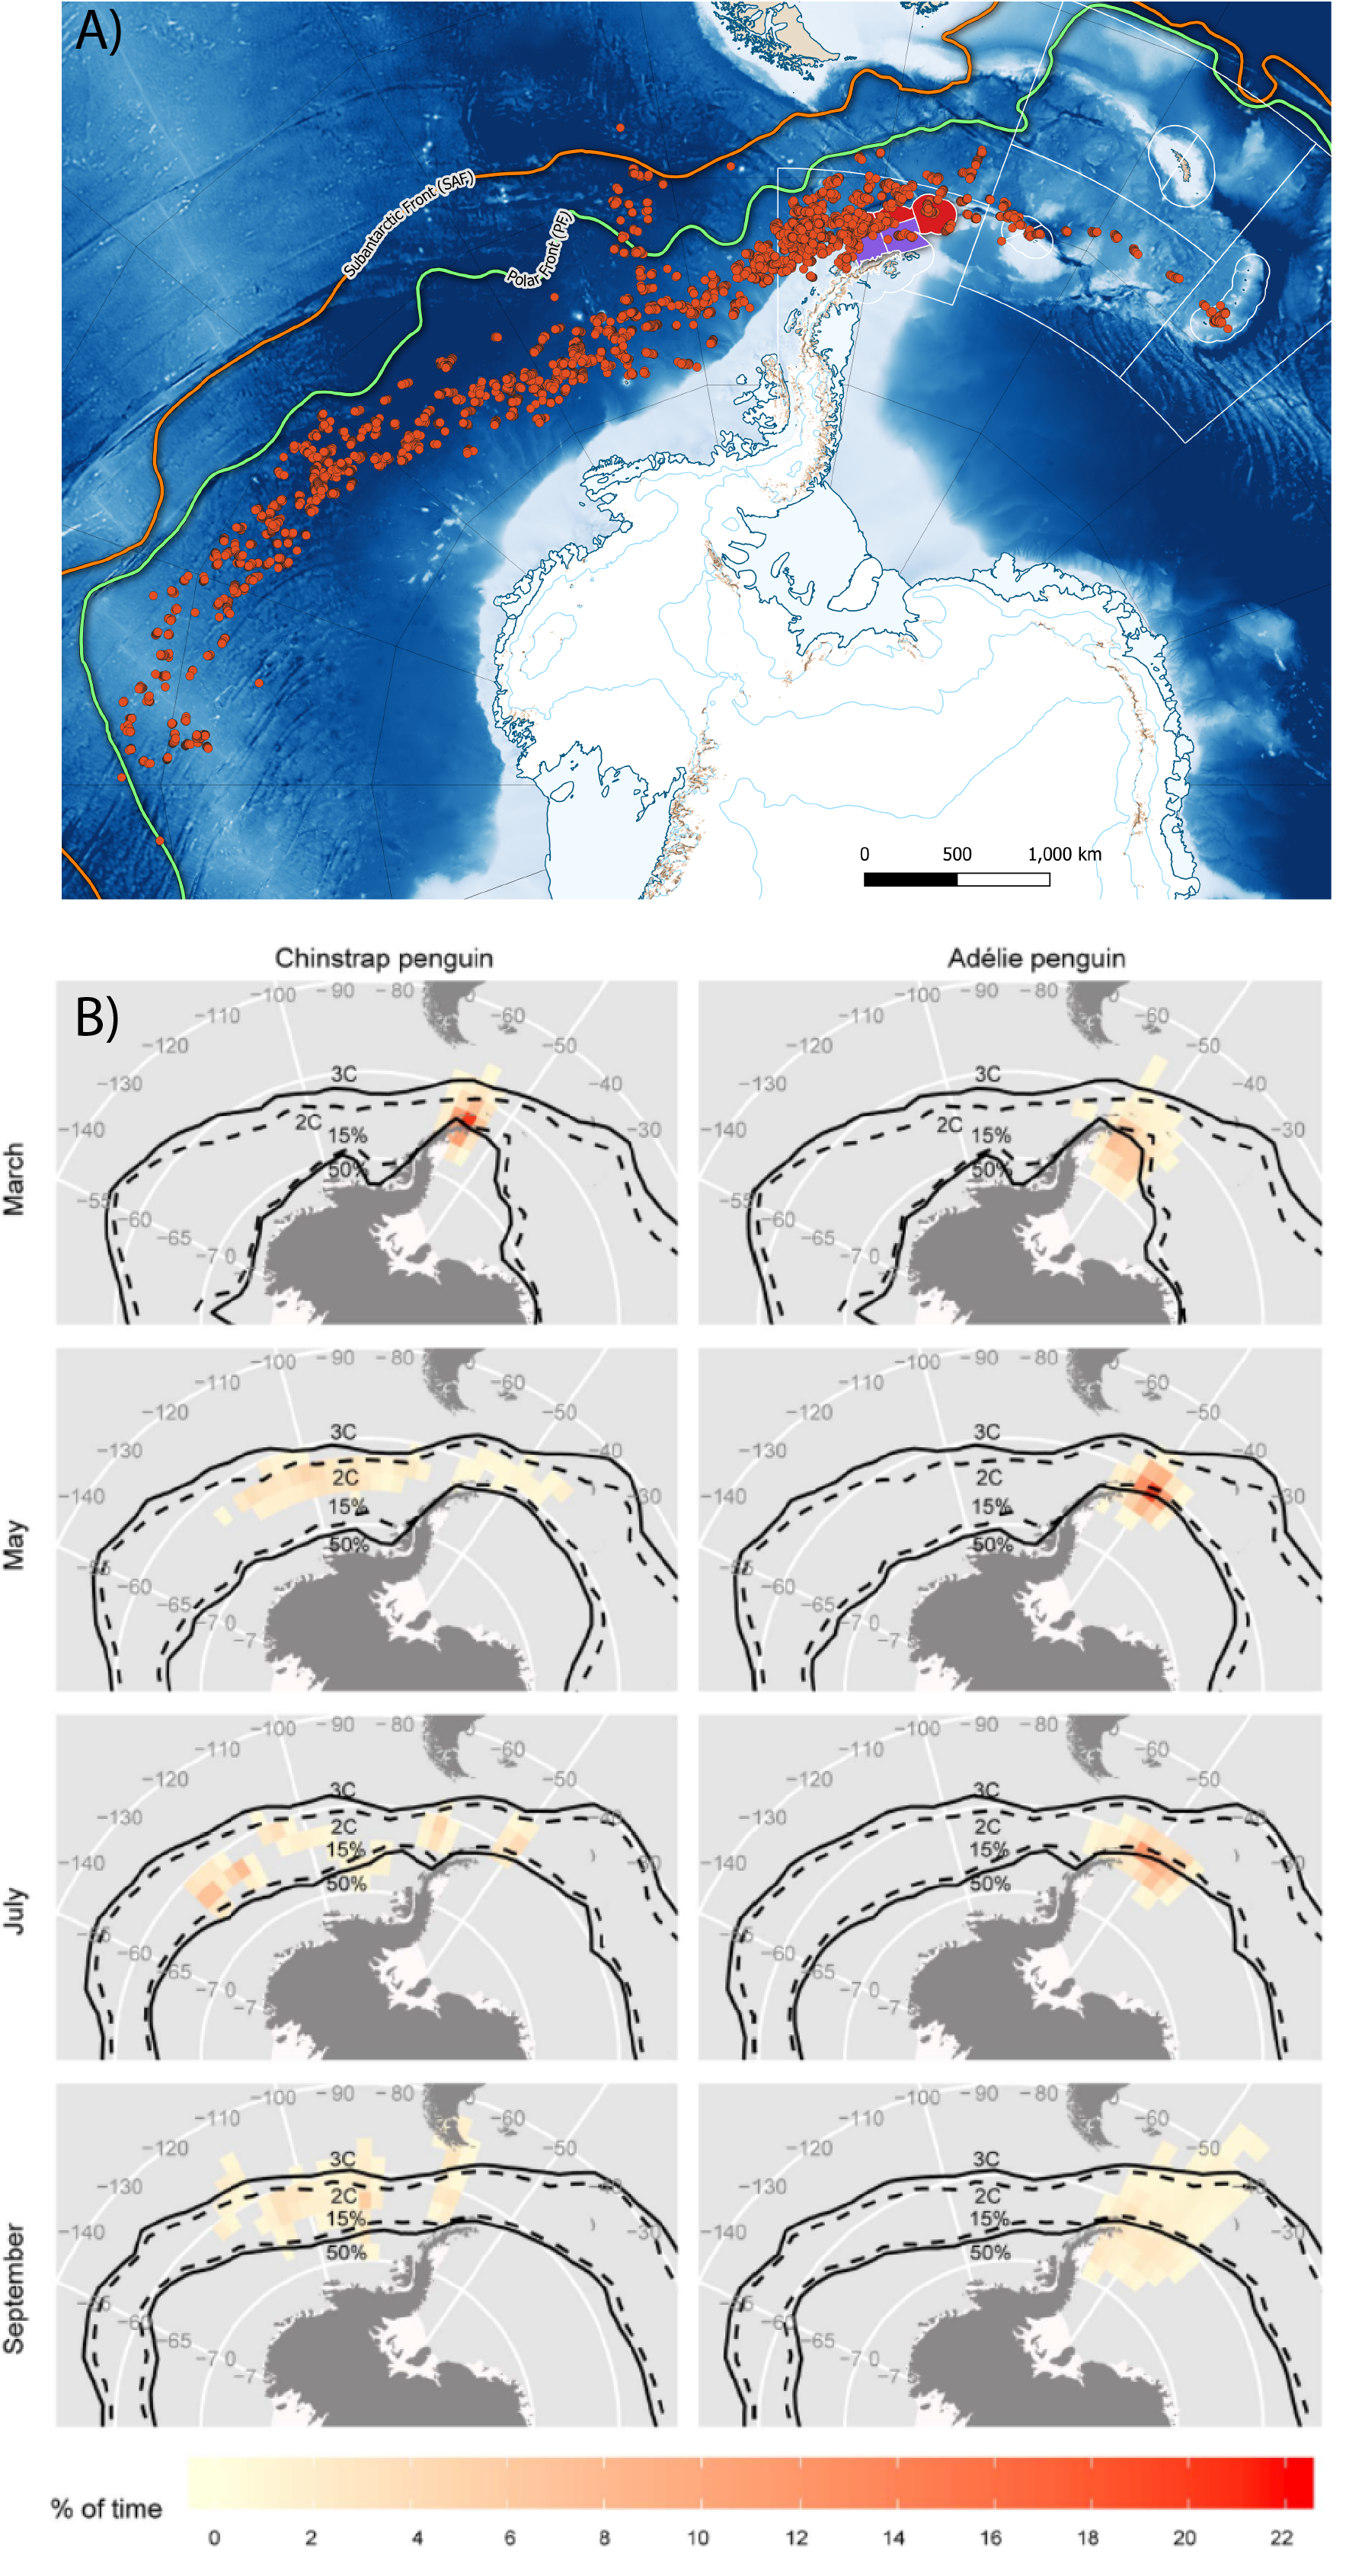
\includegraphics[width=0.75\linewidth]{./Watters EMM figures/Overwinter pengo distributions} \caption{A) Distribution of overwinter movement for chinstrap penguins, relative to the gSSMU's to which they were attributed, created from telemetry data available in Hinke et al. 2019.  B) Adélie and chinstrap penguin movement recorded by light geolocators, highlighting the large longitudinal range both species disperse through at the end of breeding (taken from Hinke et al. 2015).  In the original model formulation by Watters et al. 2020, the winter performance indices for both species are matched to macroscale levels of ONI variability but gSSMU-scale estimates of LKB and LHR.}\label{fig:Overwinter penguin  plots}
\end{figure}

\begin{figure}
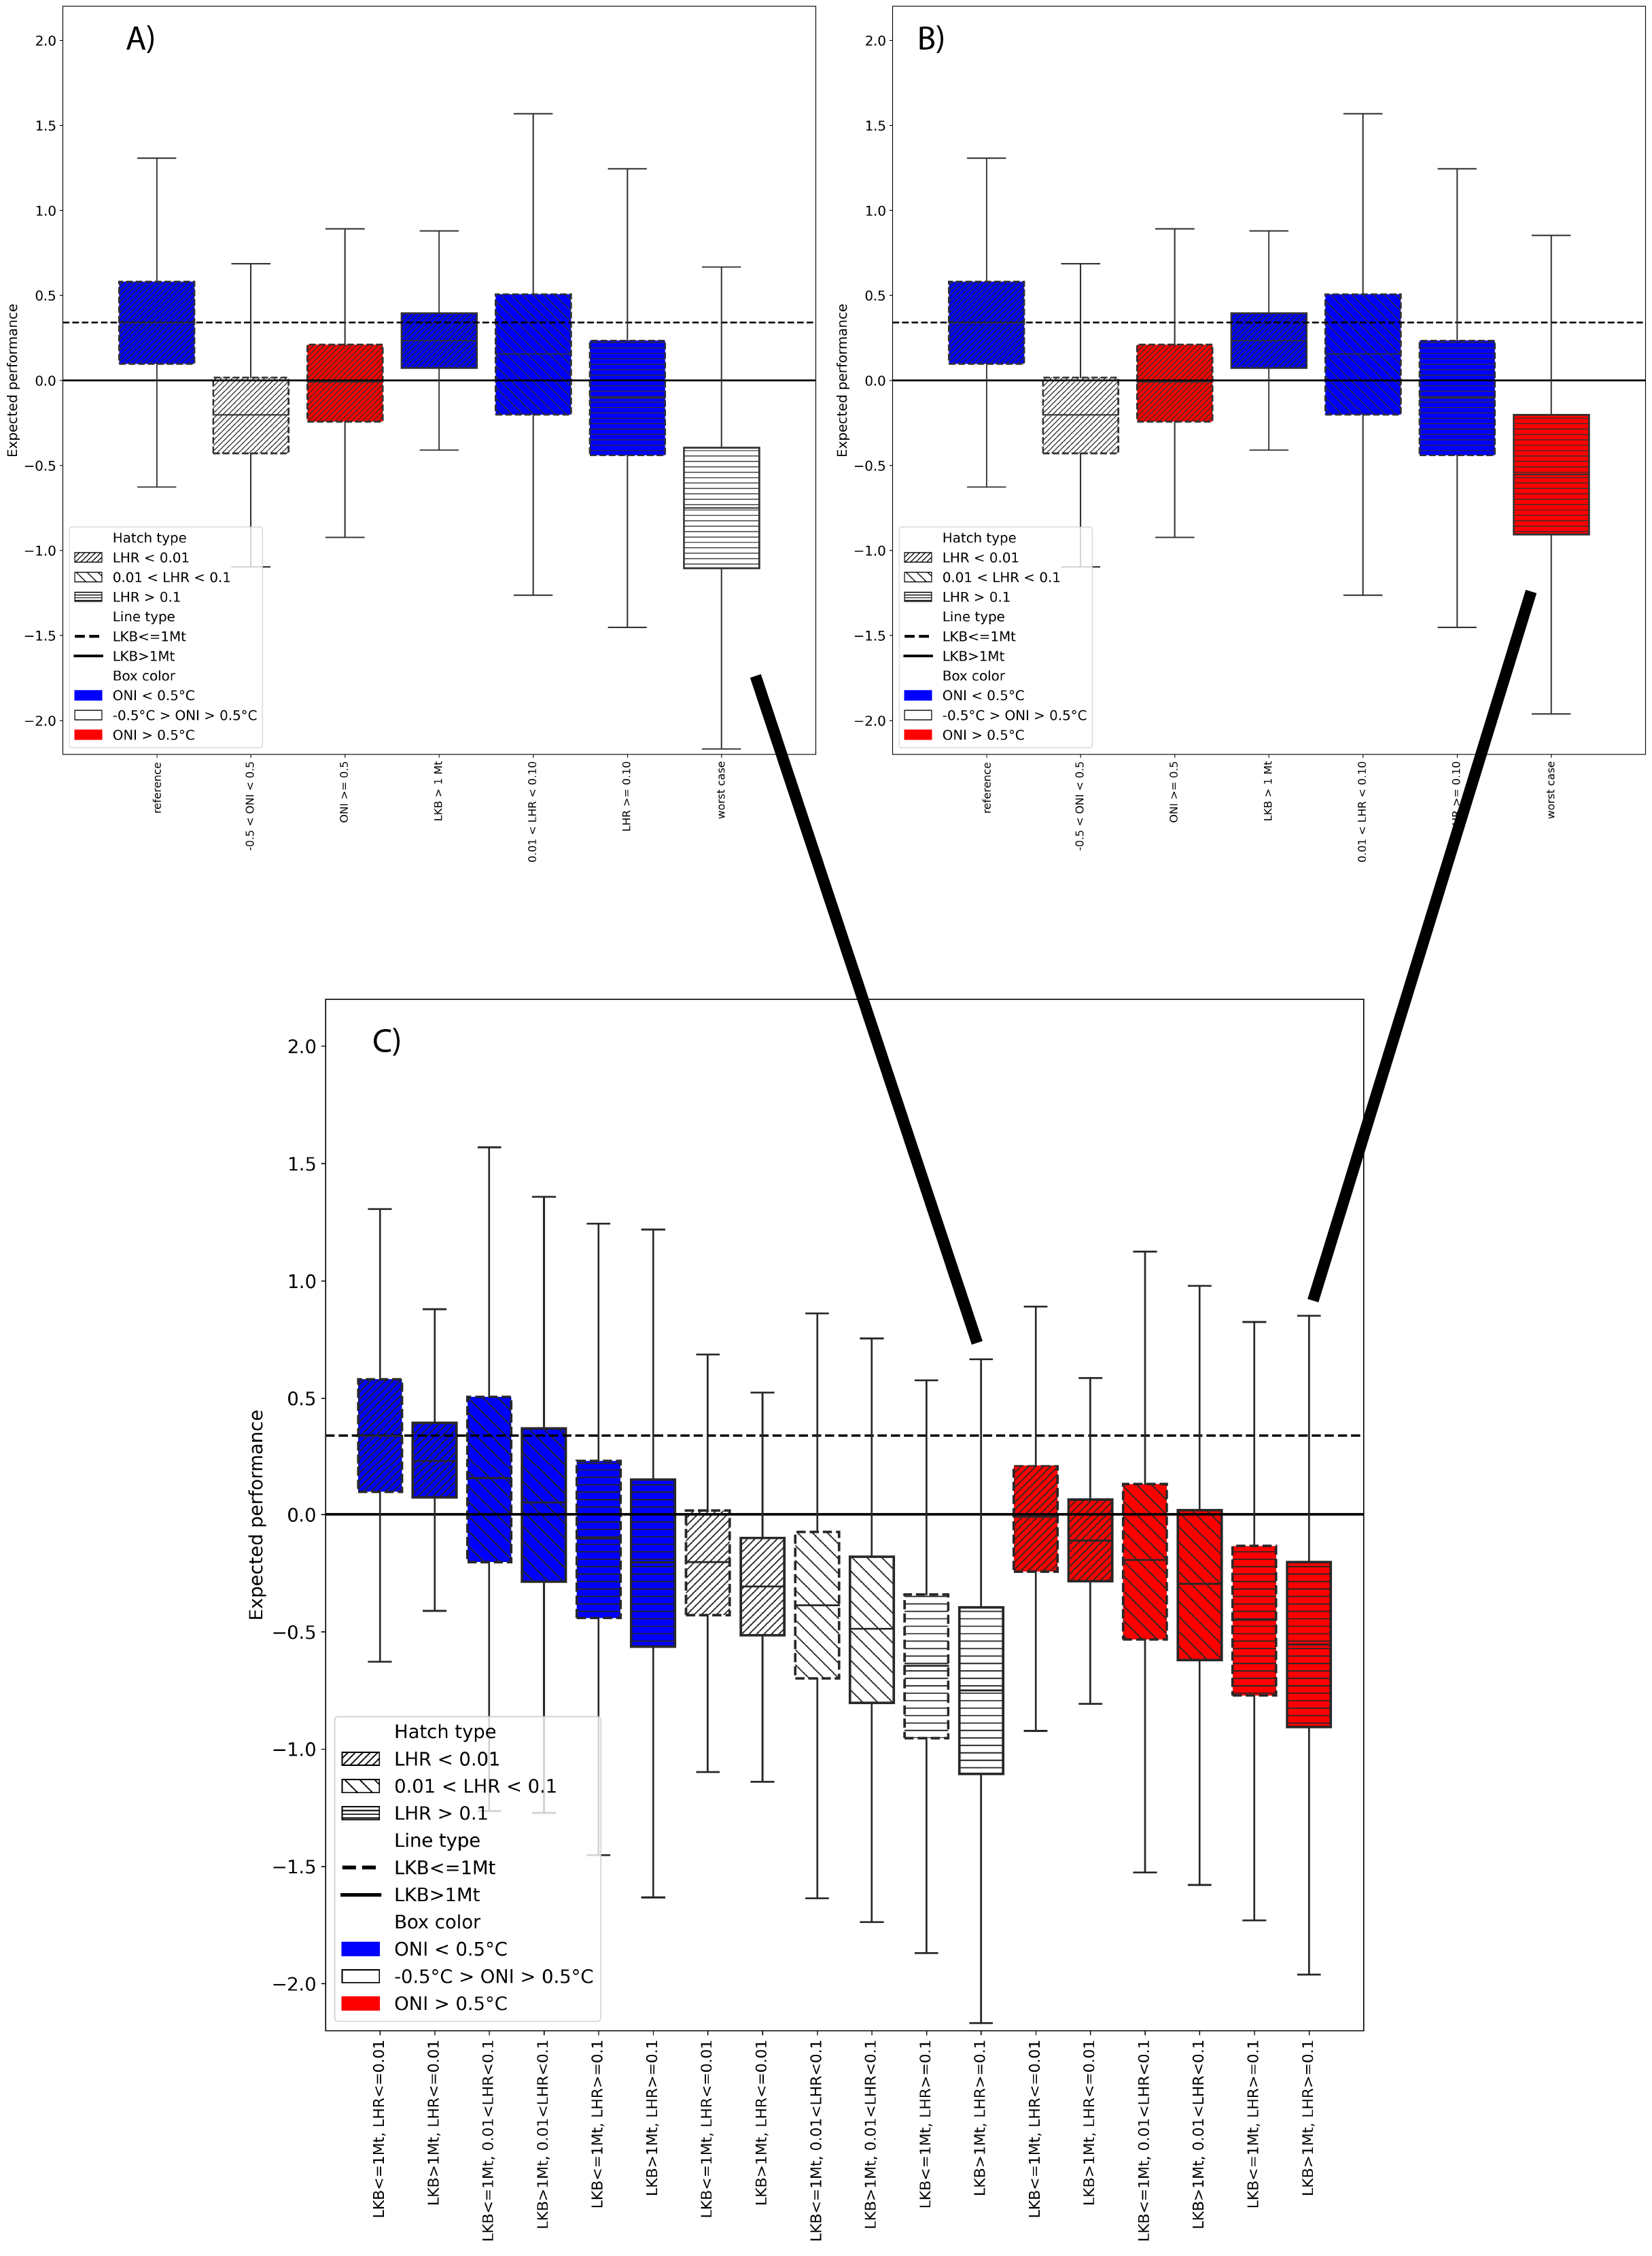
\includegraphics[width=0.75\linewidth]{./Watters EMM figures/Watters original and mistake} \caption{Original Figure 1 plot from Watters et al. 2020 with A) Neutral ONI and B) B) Warm ONI constituting the Worst Case selected.  C) Displays the original case-by-case plots recreated from the paper, with Case 12 representing the intention while data from Case 18 was selected for rendering the boxplot.  Note that the expected performance under neutral ONI Worst Case is poorer than under the warm ONI that was presented in the original paper.  Henceforth, to facilitate comparison, we refer to the ONI Neutral plot however we consider this unrealistic if the intention is to portray a Worst Case of a continuing warming climate.}\label{fig:Watters original and mistake}
\end{figure}

\begin{figure}

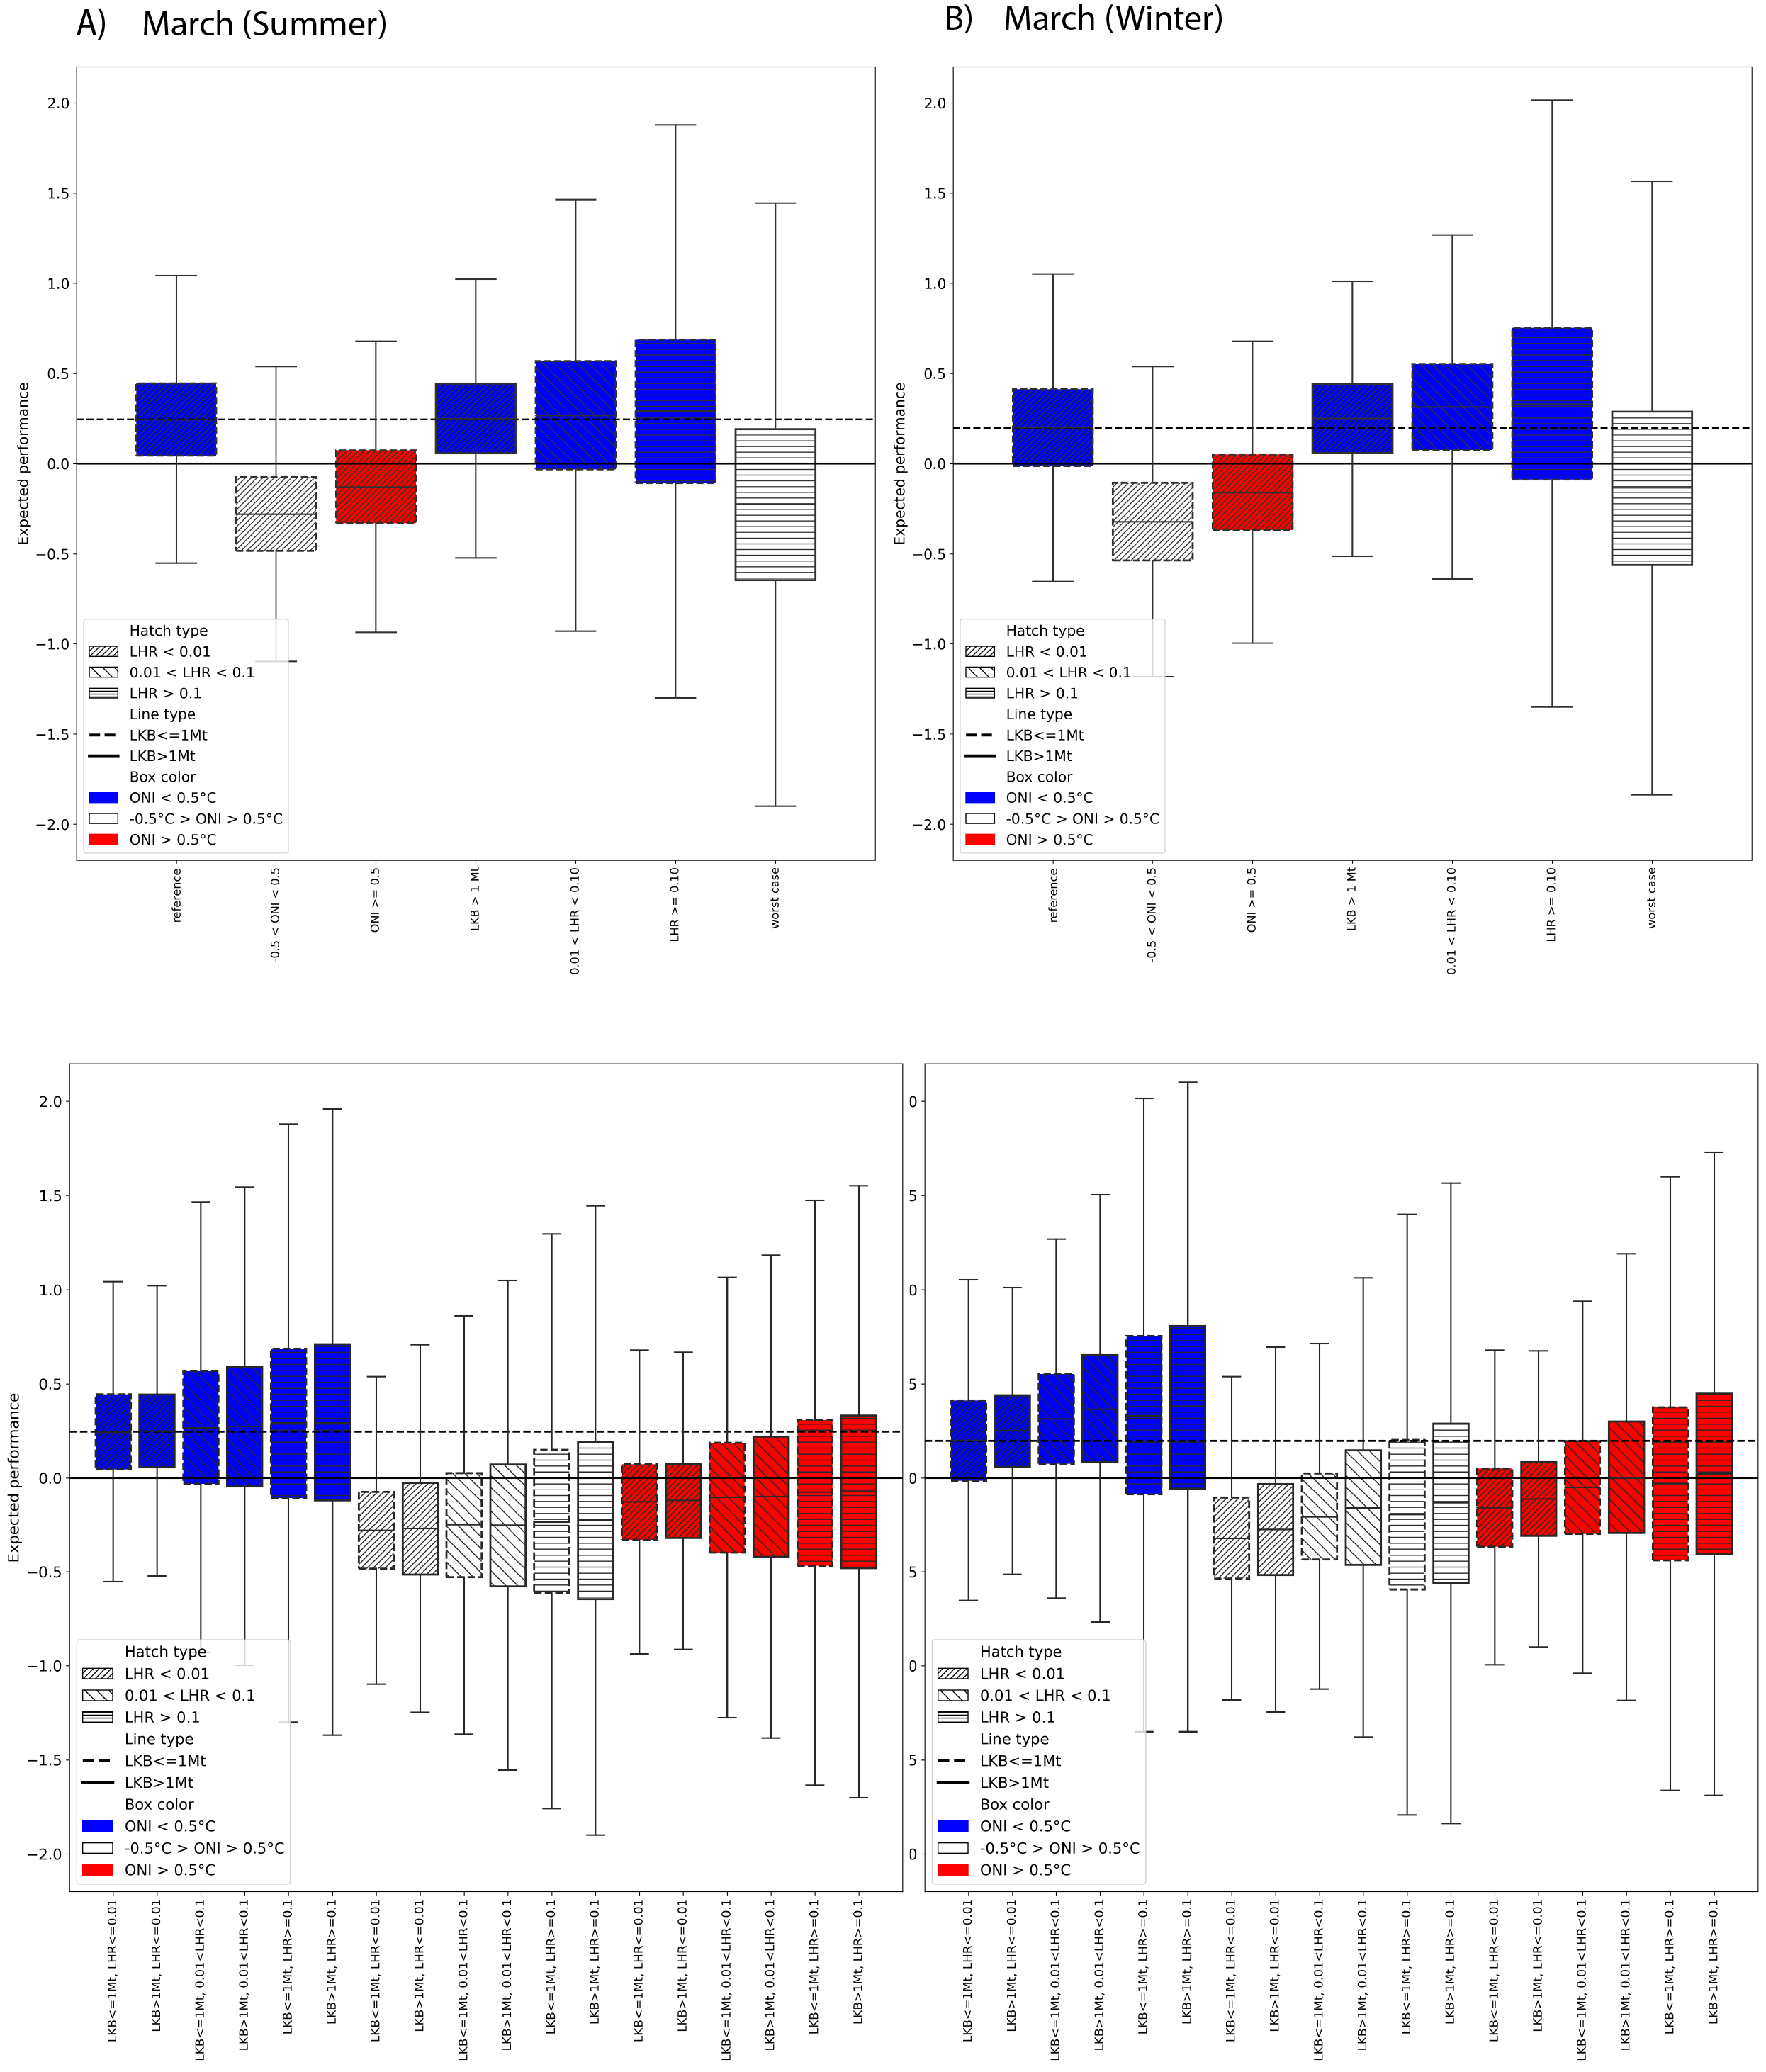
\includegraphics[width=1\linewidth]{./Watters EMM figures/All spp summer then winter 37} \hfill{}

\caption{Model output for the alternatve Watters et al. 2020 scenario outlined above (all species initially present, Adélie and chinstrap penguins migrate out of the area after breeding, LKB and LHR rescaled to SSMU and March included in summer or winter).   Selected cases as per Watters et al. 2020 for March in A) Summer and B) Winter are provided, with the corresponding case-by-case boxplots presented beneath.  Boxplots are colour-coded by ONI state (red=warm, white=neutral, blue=cold).  In all cases, the marginal effect of ONI dominated the expected performance of penguins against their long-term mean, irrespective of LKB or LHR.}\label{fig:Scenario plot 1}
\end{figure}

\begin{figure}
\centering
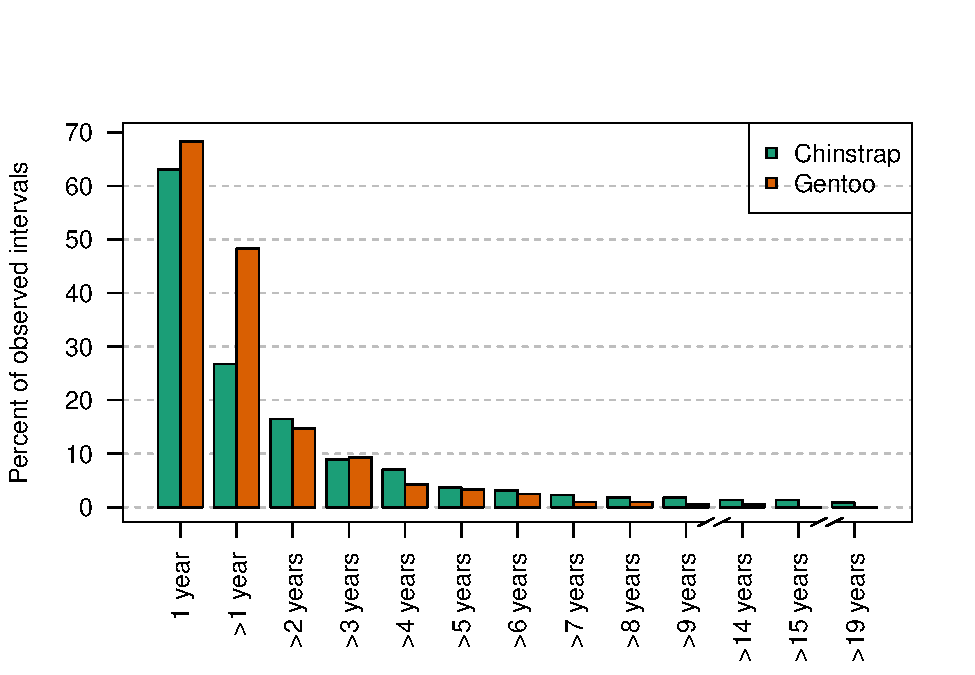
\includegraphics{WattKrug_files/figure-latex/gapCheck-1.pdf}
\caption{Frequency distribution (percent) of intervals between
consecutive breeding surveys for chinstrap and gentoo penguins, taken
from the supplementary data for Kruger et al 2021.}
\end{figure}

\begin{figure}
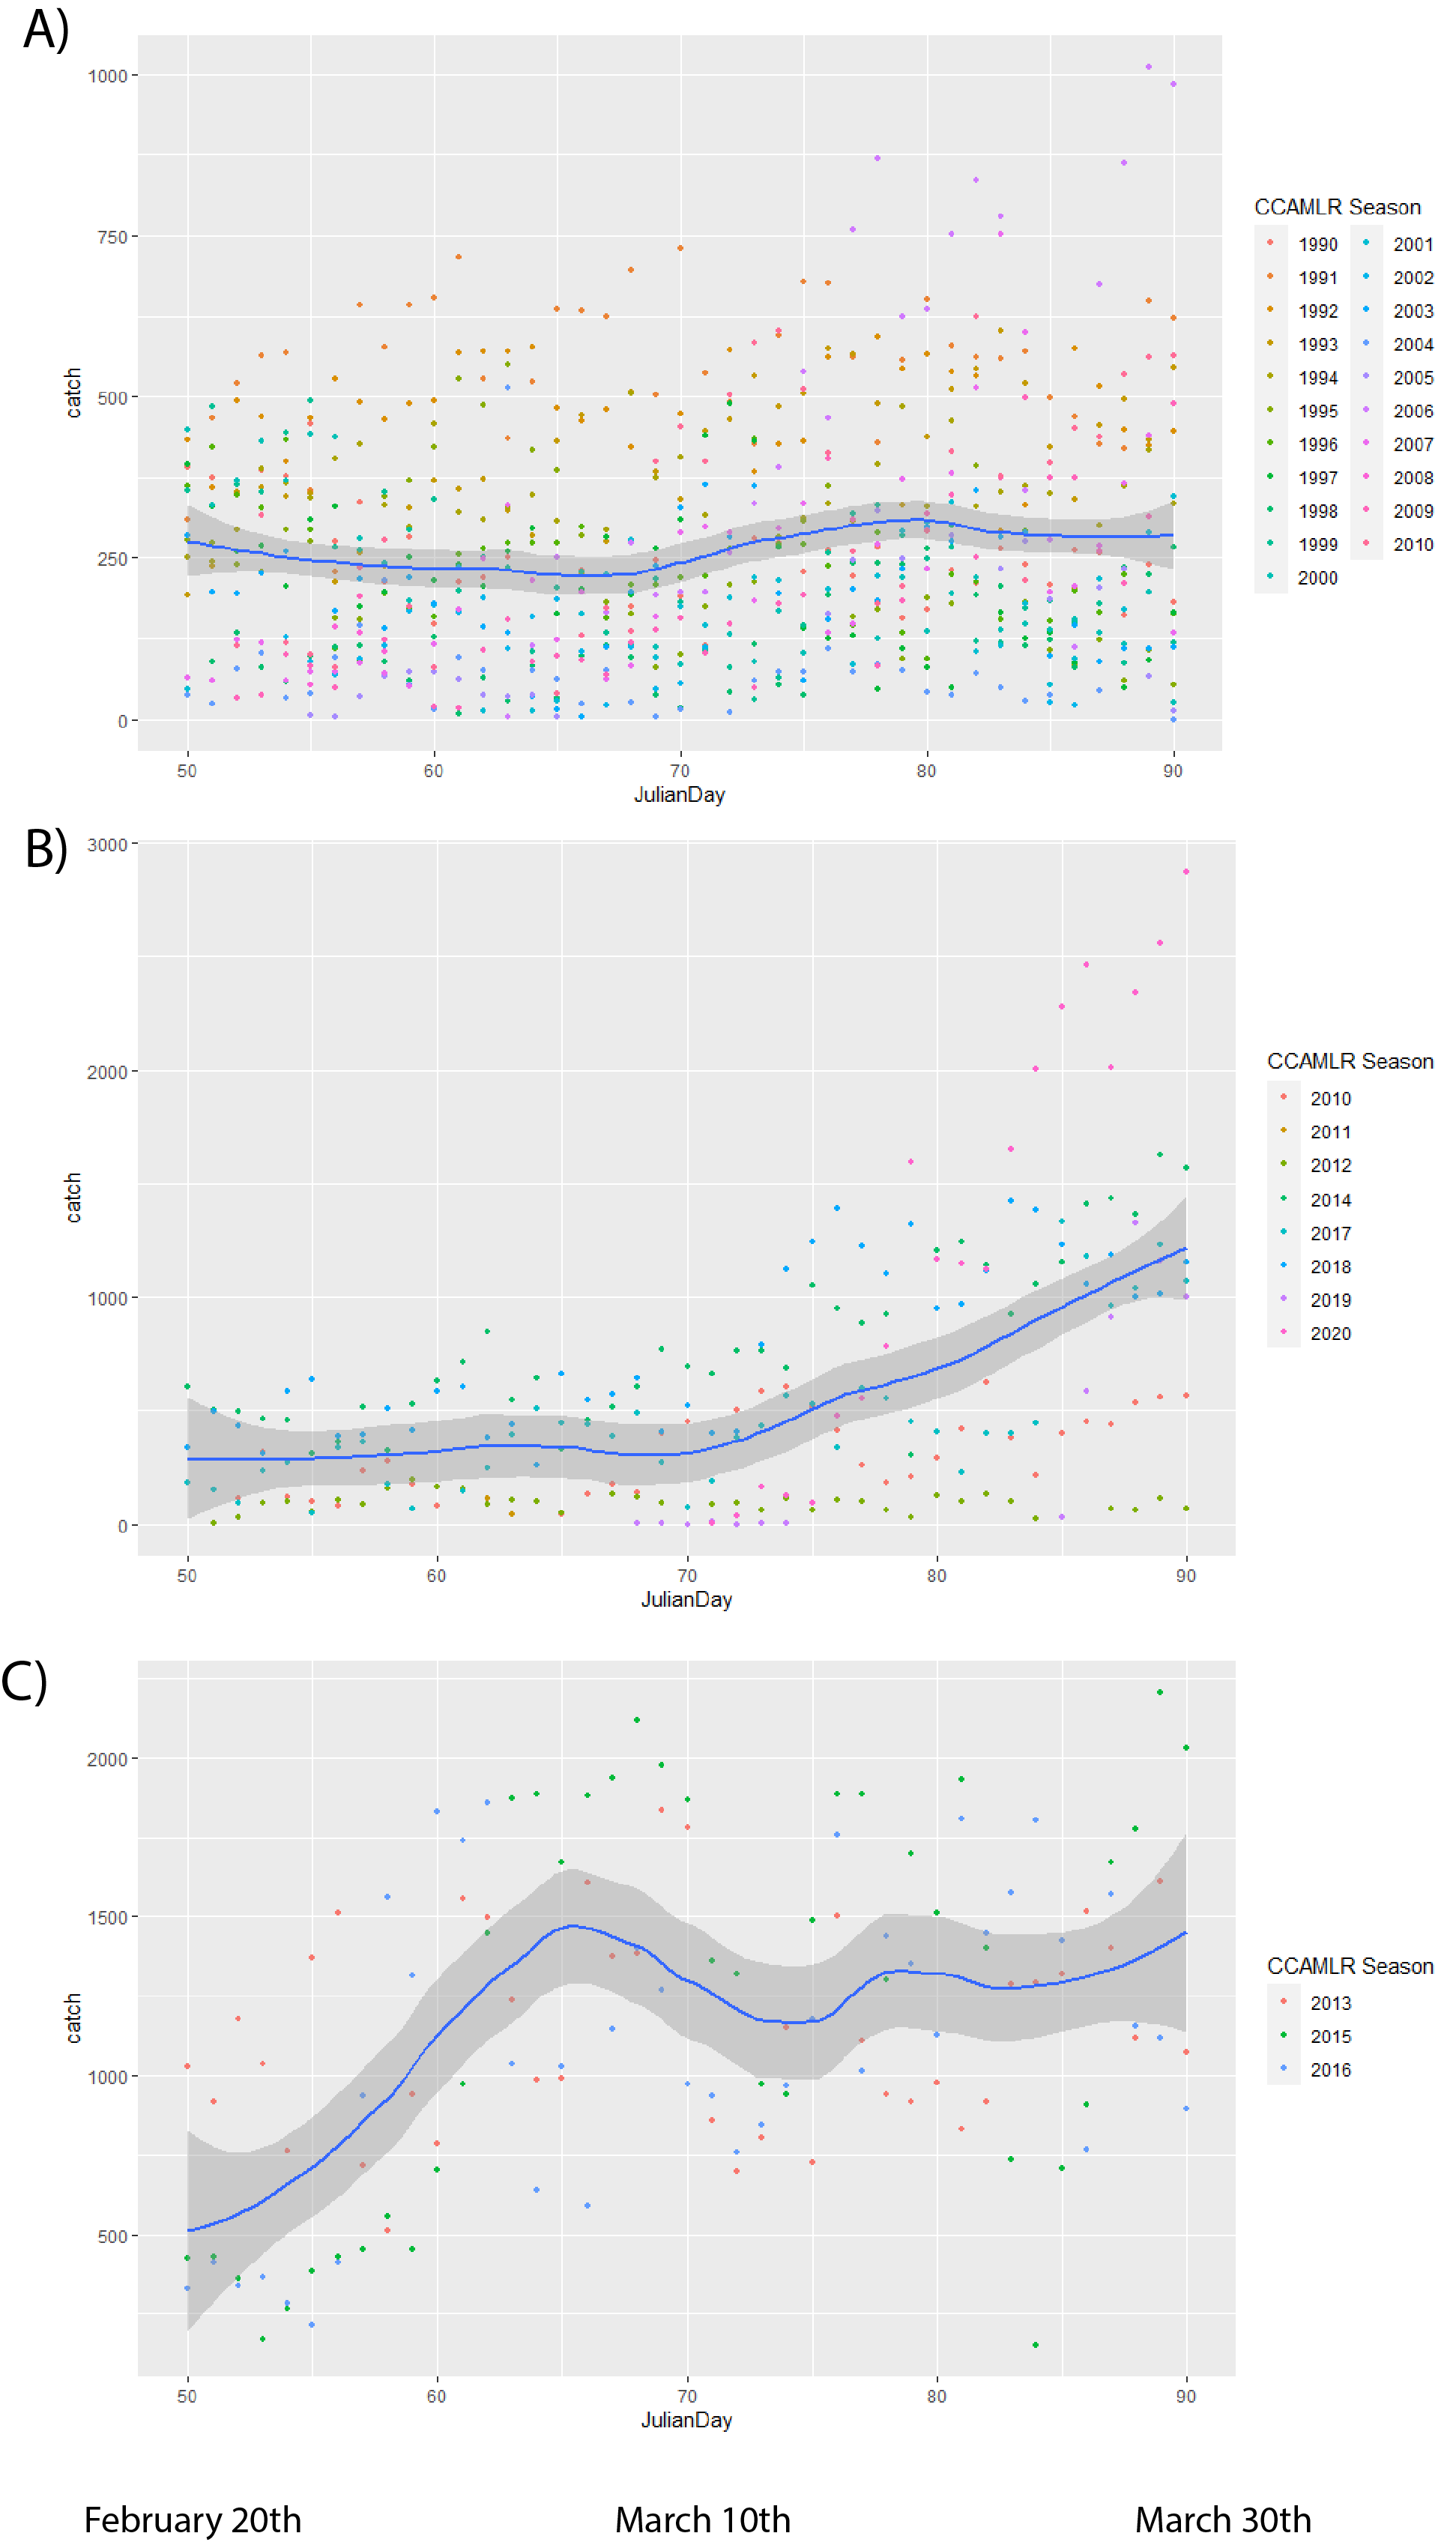
\includegraphics[width=0.6\linewidth]{./Watters EMM figures/catch march 481} \caption{Daily accumulated catch (and fitted LOESS smooth curves) in Subarea 48.1 between 20$^{th}$ February and March 31$^{st}$ between A) 1990-2010 and B) 2010 to 2020. Catch in the Subarea was relatively consistent during the latter stages of penguin breeding at approximately 250tonnes/d (NOTE: different scaling of catch on y-axis between plots).  However, since 2010 there has been a tendency for the fishery to increase its effort in the Subarea, starting around the middle of March. C) During this latter period, the fishery increased effort earlier on three occasions (2013, 2015 and 2016), starting before the beginning of March.}\label{fig:March Subarea 48.1 fishing plot}
\end{figure}
\blandscape

\begin{longtable}[t]{lccccc}
\caption{\label{tab:Table 1 Scenario Original}Original table in Watters et al. 2020.  In this and all subsequent tables below, the posterior and posterior predictive probabilities that the expected performance of penguins given the effects in the left hand column are less than the expected performance given the drivers in the column headings are provided. Worst Case is represented by neutral ONI; LHR  $\geqslant$ 0.1; and LKB $\geqslant$ 1Mt.  The Best Case is represented by La Niña conditions, low LKB and low LHR.}\\
\toprule
Effects & Best Case & -0.5 $^\circ$ C < ONI < +0.5 $^\circ$ C & ONI $\geqslant+0.5$ & Long-term $\mu$ & Long-term predicted $\mu$\\
\midrule
Best case & \- & \- & \- & 0.04 & 0.36\\
ONI Neutral & 1.00 & \- & \- & 0.89 & 0.59\\
ONI warm & 0.99 & \- & \- & 0.52 & 0.51\\
LKB High & 0.71 & 0.02 & 0.12 & 0.01 & 0.41\\
LHR medium & 0.75 & 0.16 & 0.31 & 0.32 & 0.44\\
\addlinespace
LHR high & 0.93 & 0.39 & 0.60 & 0.64 & 0.54\\
Worst case & 0.99 & \- & \- & 0.99 & 0.78\\
\bottomrule
\end{longtable}

\begin{longtable}[t]{lccccc}
\caption{\label{tab:Table 1 Scenario 37a}Posterior and posterior predictive probabilities extracted from the model output for alternatve Watters et al. 2020 scenario outlined above with March attributed to winter (Adélie and chinstrap penguins migrate out of the area after breeding, LKB and LHR rescaled to SSMU). Under this scenario, performance against the long term mean is worst for neutral and warm ONI conditions.}\\
\toprule
Effects & Best Case & -0.5 $^\circ$ C < ONI < +0.5 $^\circ$ C & ONI $\geqslant+0.5$ & Long-term $\mu$ & Long-term predicted $\mu$\\
\midrule
Best case & \- & \- & \- & 0.04 & 0.40\\
ONI Neutral & 1.00 & \- & \- & 0.97 & 0.62\\
ONI warm & 0.99 & \- & \- & 0.81 & 0.56\\
LKB High & 0.49 & 0.01 & 0.05 & 0.03 & 0.40\\
LHR medium & 0.46 & 0.04 & 0.09 & 0.14 & 0.39\\
\addlinespace
LHR high & 0.45 & 0.10 & 0.16 & 0.23 & 0.39\\
Worst case & 0.84 & \- & \- & 0.71 & 0.59\\
\bottomrule
\end{longtable}
\elandscape
\blandscape

\begin{longtable}[t]{lccccc}
\caption{\label{tab:Table 1 Scenario 37b}Posterior and posterior predictive probabilities extracted from the model output for alternatve Watters et al. 2020 scenario outlined above with March attributed to summer (Adélie and chinstrap penguins migrate out of the area after breeding, LKB and LHR rescaled to SSMU). Under this scenario performance against the long term mean is also worst for neutral and warm ONI conditions.}\\
\toprule
Effects & Best Case & -0.5 $^\circ$ C < ONI < +0.5 $^\circ$ C & ONI $\geqslant+0.5$ & Long-term $\mu$ & Long-term predicted $\mu$\\
\midrule
Best case & \- & \- & \- & 0.10 & 0.42\\
ONI Neutral & 1.00 & \- & \- & 0.98 & 0.63\\
ONI warm & 0.99 & \- & \- & 0.86 & 0.56\\
LKB High & 0.40 & 0.00 & 0.04 & 0.03 & 0.40\\
LHR medium & 0.27 & 0.01 & 0.02 & 0.04 & 0.37\\
\addlinespace
LHR high & 0.37 & 0.08 & 0.13 & 0.21 & 0.38\\
Worst case & 0.76 & \- & \- & 0.63 & 0.55\\
\bottomrule
\end{longtable}

\elandscape
\blandscape

\elandscape
\blandscape

\elandscape

\newpage  
\beginsupplement
\blandscape

\hypertarget{supplementary-material}{%
\section{Supplementary material}\label{supplementary-material}}

\begin{figure}
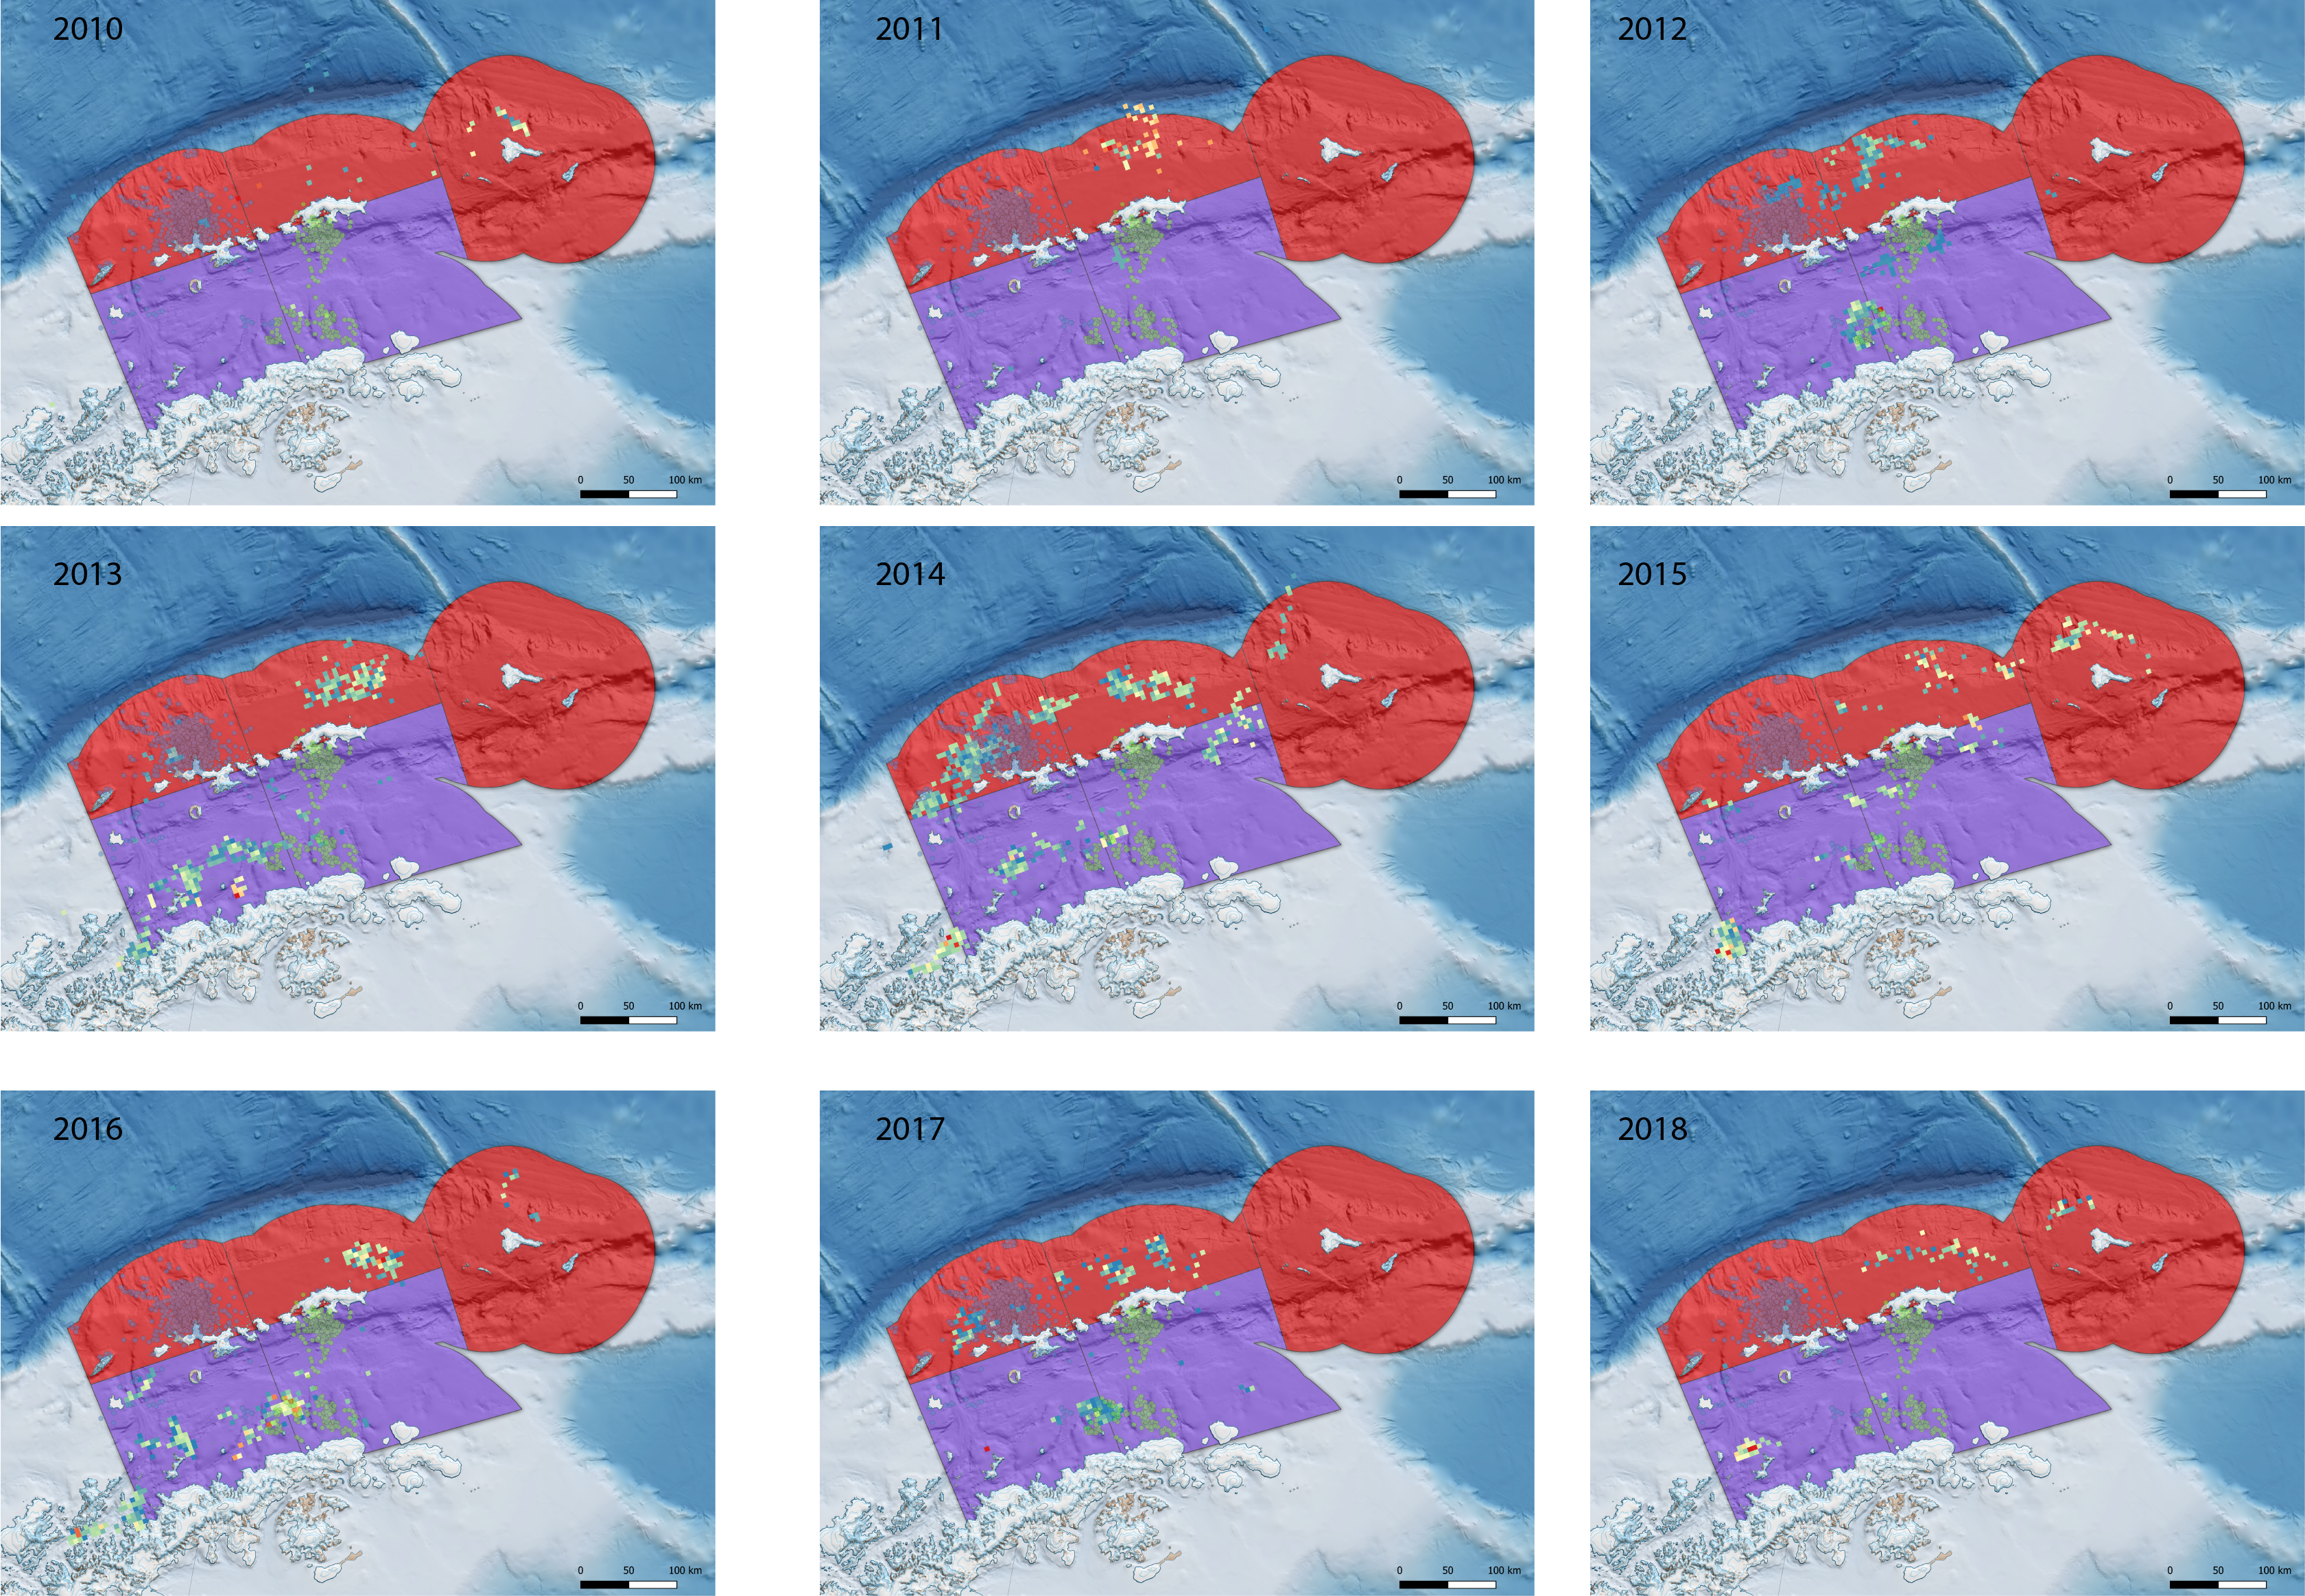
\includegraphics[width=0.8\linewidth]{./Watters EMM figures/summer catch/Year by year catch} \caption{C1 Catch and Effort data for 2010 - 2018, for all catches during the period of the austral summer relating to Adélie and chinstrap penguins in Subarea 48.1 (i.e. up to $10^{th}$ March).  The telemetry data presented in Hinke et al. 2017 for chinstrap penguins at both Cape Shireff and Copacabana and the gSSMU used in the Watters et al. 2020 paper are superimposed to highlight the extreme variability in actual catch, relative to the scale of LHR used to reflect interactions with penguins.  Our reanalysis re-scaled LHR to the SSMU level, though we contend that for the purposes of matching predator data at appropriate spatial scales even this is too coarse a resolution.}\label{fig:Supplementary Figure 1}
\end{figure}
\elandscape
\begin{figure}

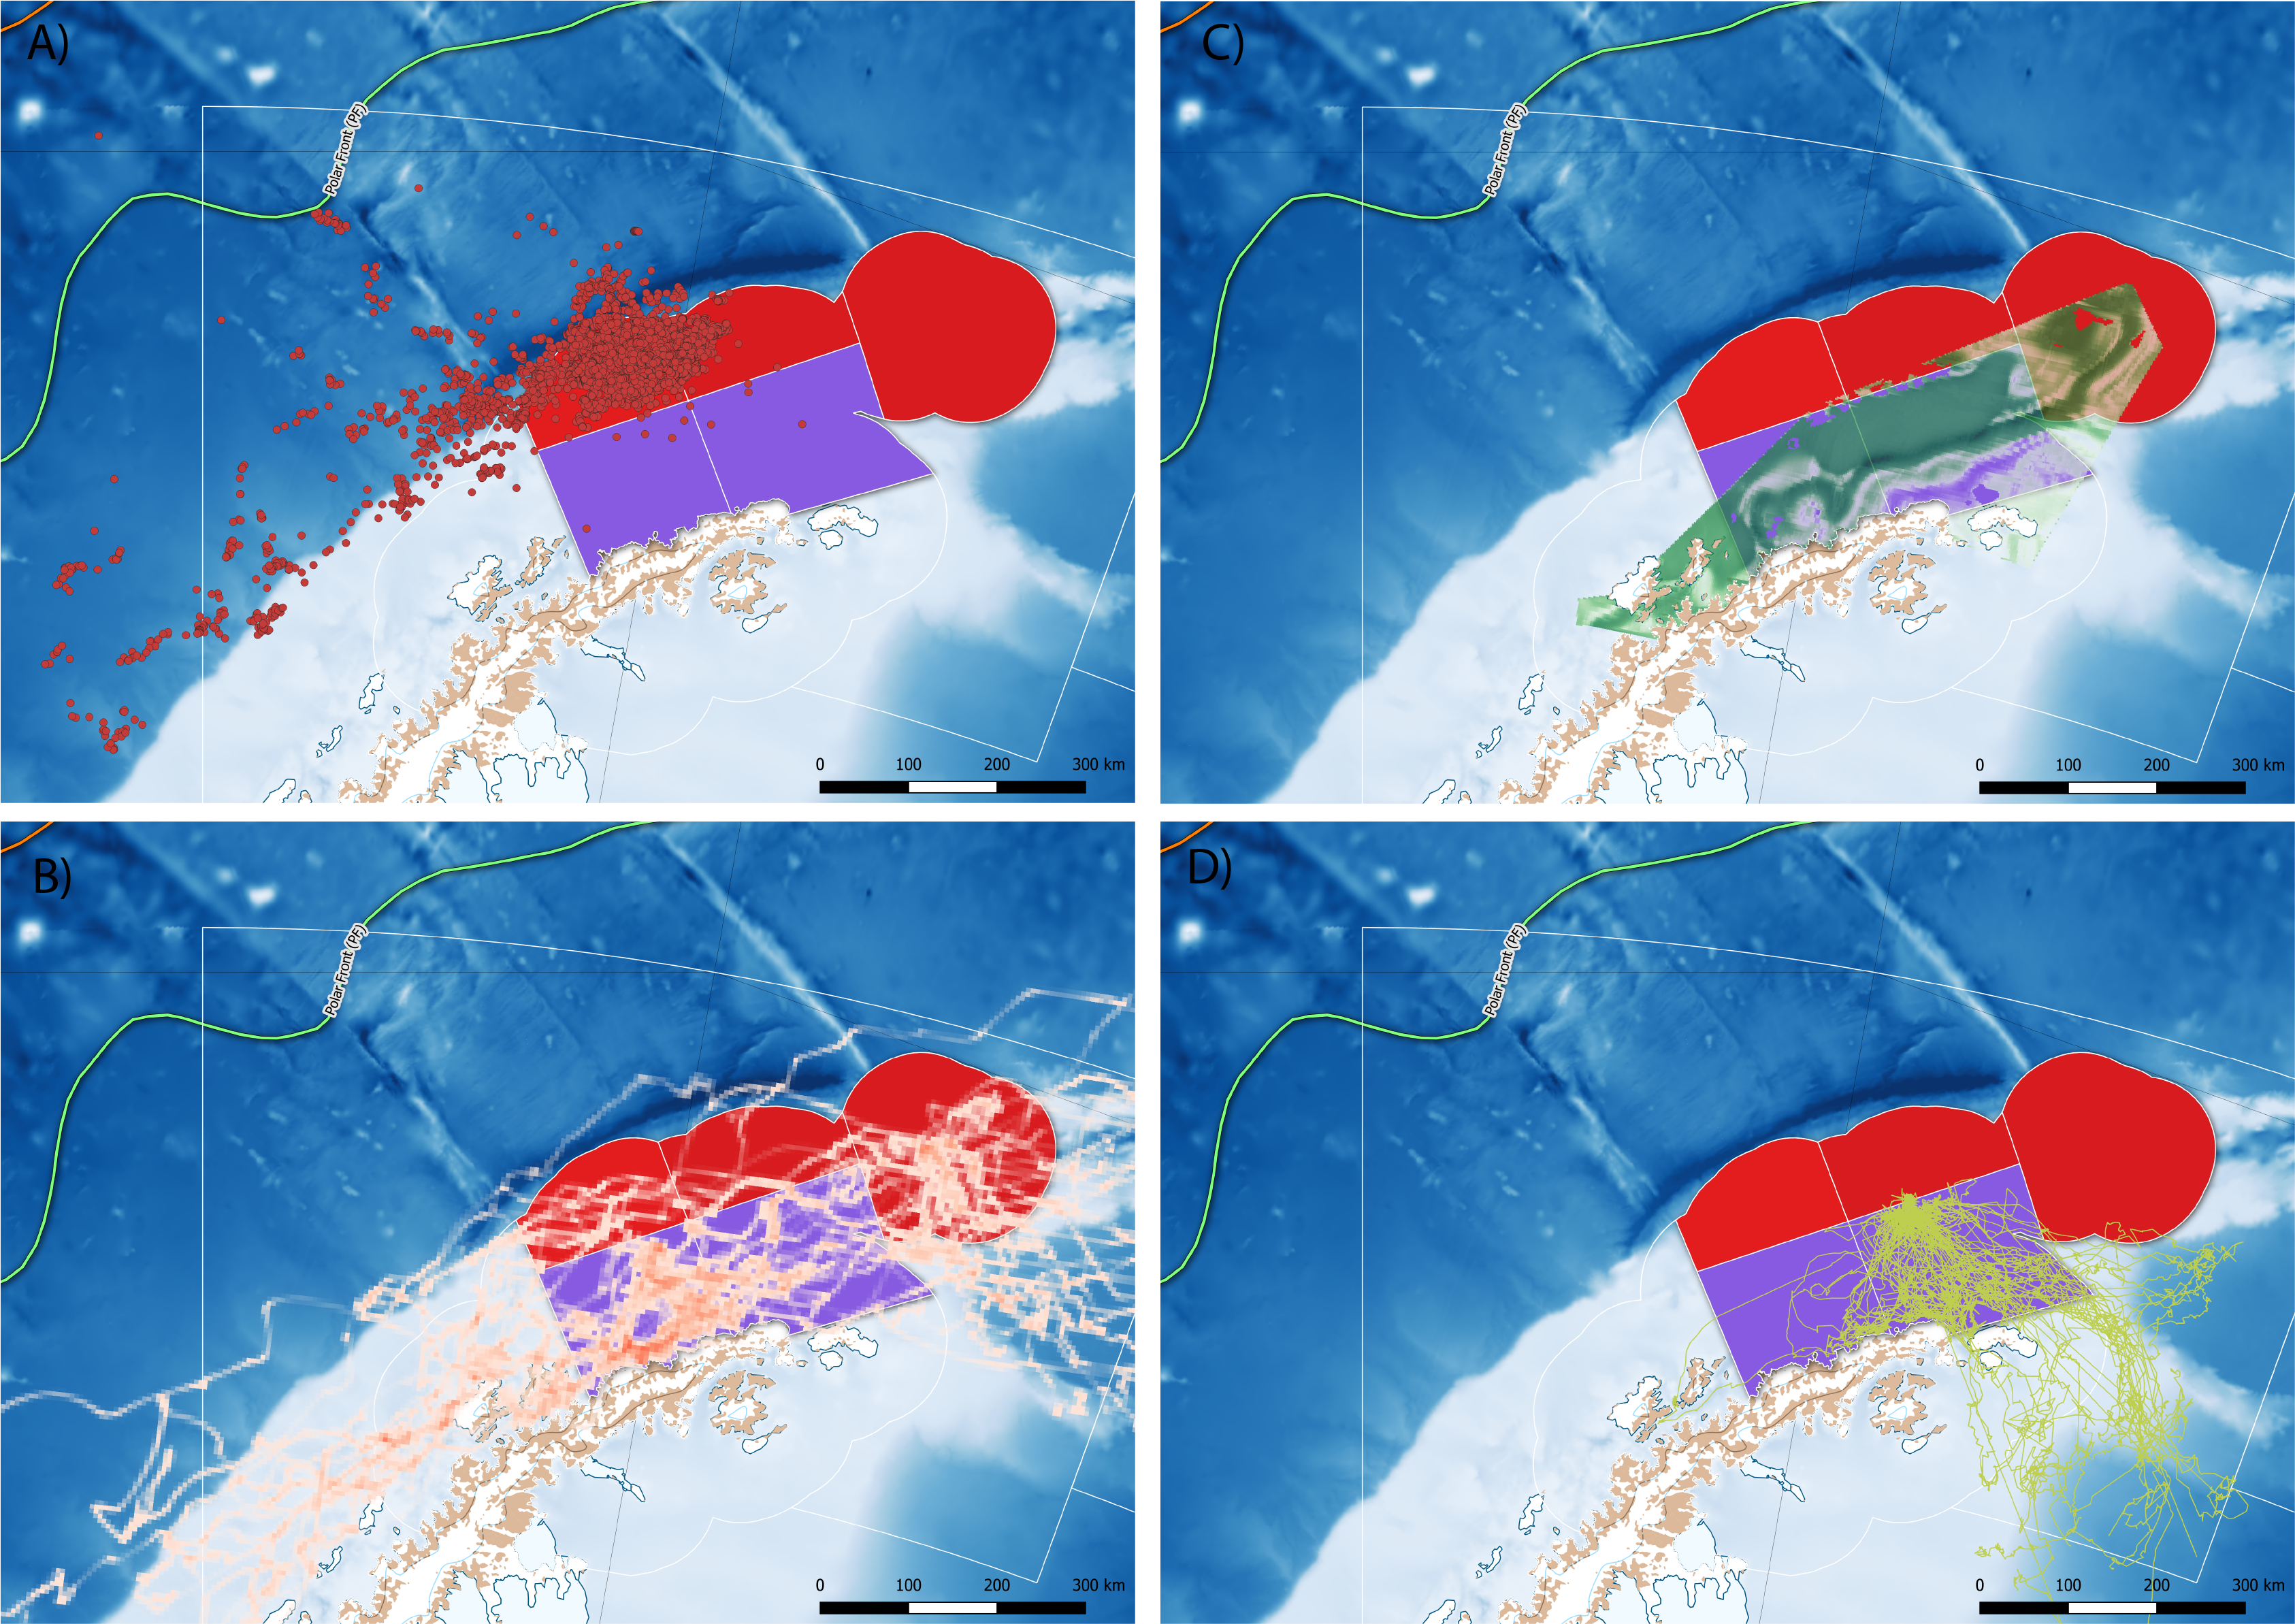
\includegraphics[width=1\linewidth]{./Watters EMM figures/Other spp distribution} \hfill{}

\caption{The summer distribution of foraging effort by A) adult female Antarctic fur seals (adapted from telemetry data available in Hinke et al. 2017), B) migratory adult male Antarctic fur seals (adapted from Lowther et al. 2020) C) humpback whales throughout December (adapted from Johannessen et al., this meeting) and D) nonbreeding adult Adélie penguins during the breeding season (adapted from data in Oosthuizen et al., this meeting). Potential effects of competitive overlap between pygoscelid penguins and other krill dependent predators, particularly those who have increased their abundance dramatically over the preceding 40 years, are excluded from both approaches, creating an unrealistic set of boundary conditions for interpreting the variance in penguin vital rates.}\label{fig:Supplementary Figure 2 other species plots}
\end{figure}
\newpage
\scriptsize

\begin{Shaded}
\begin{Highlighting}[numbers=left,,]
\CommentTok{####DATA PREP AND MODEL CODE (IMPUTATION OF BIOMASS = TRUE)----}
\CommentTok{#original paper here:}
\NormalTok{https}\OperatorTok{:}\ErrorTok{//}\NormalTok{doi.org}\OperatorTok{/}\FloatTok{10.1038}\OperatorTok{/}\NormalTok{s41598}\DecValTok{-020-59223-9}
\CommentTok{#requirements - raw Supplementary Files from original Watters et al. (2020) publication available here:}
\NormalTok{https}\OperatorTok{:}\ErrorTok{//}\NormalTok{www.nature.com}\OperatorTok{/}\NormalTok{articles}\OperatorTok{/}\NormalTok{s41598}\DecValTok{-020-59223-9}\CommentTok{#Sec8}
\CommentTok{# the analyses with imputation takes several hours - the scenarios outlined in the paper are provided as .csv}
\CommentTok{# files in the Zenodo repository provided which is open access via the DOI here (https://doi.org/10.5281/zenodo.5040114)}
\CommentTok{# and provided in the manuscript.}
\CommentTok{# the raw files to conduct the analyses from first prinicples are also available from the Watters et al.2020 manuscript }
\CommentTok{#SCRIPT MODIFICATIONS:}
\CommentTok{#L. 225 - 233.  These changes modify the Acoustic biomass estimates by the ratio of SSMU / gSSMU}
\CommentTok{#L. 253.  Alter March to either Summer or Winter.  Currently set to Winter.}
\CommentTok{#L. 255 - 258.  Modify the gSSMU configurations to reflect only SSMU}
\CommentTok{#L. 284, 286 & 290.  Set CHPE and ADPE in WINTER to NA - removing from model / migration out of area}
\CommentTok{#L. 666.  Incorrect parameter set selection for "Worst Case" Fig 2 / "Selected Cases" plot.}
\KeywordTok{library}\NormalTok{(tidyverse)}
\NormalTok{make.localhr.data<-}\ControlFlowTok{function}\NormalTok{(}\DataTypeTok{trim=}\DecValTok{1}\NormalTok{,}\DataTypeTok{plot.winter=}\OtherTok{FALSE}\NormalTok{)\{}
  \CommentTok{# fledge weight (fwt)}
  \CommentTok{# bigger indicates better summer}
\NormalTok{  fwt<-}\KeywordTok{read.csv}\NormalTok{(}\StringTok{"fweight.csv"}\NormalTok{,}\DataTypeTok{header=}\OtherTok{TRUE}\NormalTok{,}\DataTypeTok{stringsAsFactors =} \OtherTok{FALSE}\NormalTok{)}
\NormalTok{  fwt<-}\KeywordTok{tapply}\NormalTok{(fwt}\OperatorTok{$}\NormalTok{WT,}\KeywordTok{list}\NormalTok{(fwt}\OperatorTok{$}\NormalTok{YEAR,fwt}\OperatorTok{$}\NormalTok{PROJECT,fwt}\OperatorTok{$}\NormalTok{SPECIES),mean)}
\NormalTok{  fwt<-}\KeywordTok{data.frame}\NormalTok{(}\DataTypeTok{YEAR=}\KeywordTok{rep}\NormalTok{(}\KeywordTok{dimnames}\NormalTok{(fwt)[[}\DecValTok{1}\NormalTok{]],}\KeywordTok{dim}\NormalTok{(fwt)[}\DecValTok{2}\NormalTok{]}\OperatorTok{*}\KeywordTok{dim}\NormalTok{(fwt)[}\DecValTok{3}\NormalTok{]),}
                  \DataTypeTok{PROJECT=}\KeywordTok{rep}\NormalTok{(}\KeywordTok{rep}\NormalTok{(}\KeywordTok{dimnames}\NormalTok{(fwt)[[}\DecValTok{2}\NormalTok{]],}\DataTypeTok{each=}\KeywordTok{dim}\NormalTok{(fwt)[}\DecValTok{1}\NormalTok{]),}\KeywordTok{dim}\NormalTok{(fwt)[}\DecValTok{3}\NormalTok{]),}
                  \DataTypeTok{SPECIES=}\KeywordTok{rep}\NormalTok{(}\KeywordTok{dimnames}\NormalTok{(fwt)[[}\DecValTok{3}\NormalTok{]],}\DataTypeTok{each=}\KeywordTok{dim}\NormalTok{(fwt)[}\DecValTok{1}\NormalTok{]}\OperatorTok{*}\KeywordTok{dim}\NormalTok{(fwt)[}\DecValTok{2}\NormalTok{]),}
                  \DataTypeTok{fwt=}\KeywordTok{c}\NormalTok{(fwt),}\DataTypeTok{stringsAsFactors =} \OtherTok{FALSE}\NormalTok{)}
\NormalTok{  fwt}\OperatorTok{$}\NormalTok{matchme<-}\KeywordTok{paste}\NormalTok{(fwt}\OperatorTok{$}\NormalTok{PROJECT,fwt}\OperatorTok{$}\NormalTok{SPECIES,}\DataTypeTok{sep=}\StringTok{"|"}\NormalTok{)}
\NormalTok{  tt<-}\KeywordTok{tapply}\NormalTok{(fwt}\OperatorTok{$}\NormalTok{fwt,}\KeywordTok{list}\NormalTok{(fwt}\OperatorTok{$}\NormalTok{matchme),mean,}\DataTypeTok{na.rm=}\OtherTok{TRUE}\NormalTok{)}
\NormalTok{  ttt<-}\KeywordTok{tapply}\NormalTok{(fwt}\OperatorTok{$}\NormalTok{fwt,}\KeywordTok{list}\NormalTok{(fwt}\OperatorTok{$}\NormalTok{matchme),sd,}\DataTypeTok{na.rm=}\OtherTok{TRUE}\NormalTok{)}
\NormalTok{  mean.fwt<-tt[}\KeywordTok{match}\NormalTok{(fwt}\OperatorTok{$}\NormalTok{matchme,}\KeywordTok{names}\NormalTok{(tt))]}
\NormalTok{  sd.fwt<-ttt[}\KeywordTok{match}\NormalTok{(fwt}\OperatorTok{$}\NormalTok{matchme,}\KeywordTok{names}\NormalTok{(ttt))]}
\NormalTok{  fwt}\OperatorTok{$}\NormalTok{std.mean.fwt<-(fwt}\OperatorTok{$}\NormalTok{fwt}\OperatorTok{-}\NormalTok{mean.fwt)}\OperatorTok{/}\NormalTok{sd.fwt}
\NormalTok{  fwt<-fwt[,}\OperatorTok{-}\KeywordTok{c}\NormalTok{(}\DecValTok{4}\OperatorTok{:}\DecValTok{5}\NormalTok{)]}
  \CommentTok{#omits<-(fwt$SPECIES=="ADPE"&fwt$PROJECT=="CS")|(fwt$SPECIES=="CHPE"&fwt$PROJECT=="COPA")}
  \CommentTok{#fwt<-fwt[!omits,]}
  \KeywordTok{names}\NormalTok{(fwt)[}\DecValTok{4}\NormalTok{]<-}\StringTok{"index"}
\NormalTok{  fwt}\OperatorTok{$}\NormalTok{param=}\KeywordTok{rep}\NormalTok{(}\StringTok{"FWT"}\NormalTok{,}\KeywordTok{dim}\NormalTok{(fwt)[}\DecValTok{1}\NormalTok{])}
\NormalTok{  fwt}\OperatorTok{$}\NormalTok{season=}\KeywordTok{rep}\NormalTok{(}\StringTok{"S"}\NormalTok{,}\KeywordTok{dim}\NormalTok{(fwt)[}\DecValTok{1}\NormalTok{])}
  \CommentTok{# make stuff reference the correct "calendar year" for matching up with krill survey and catch data}
  \CommentTok{# summer indices are relevant to the second year in the split-season designation}
\NormalTok{  fwt}\OperatorTok{$}\NormalTok{cal.yr<-}\KeywordTok{as.numeric}\NormalTok{(}\KeywordTok{substr}\NormalTok{(fwt}\OperatorTok{$}\NormalTok{YEAR,}\DecValTok{1}\NormalTok{,}\DecValTok{4}\NormalTok{))}\OperatorTok{+}\DecValTok{1}
  \CommentTok{#print(str(fwt))}
  \CommentTok{#}
  \CommentTok{# post-hatch success (phs) (numbers of chicks creched/numbers of chicks hatched)}
  \CommentTok{# bigger indicates better summer}
\NormalTok{  phs<-}\KeywordTok{read.csv}\NormalTok{(}\StringTok{"success.csv"}\NormalTok{,}\DataTypeTok{header=}\OtherTok{TRUE}\NormalTok{,}\DataTypeTok{stringsAsFactors =} \OtherTok{FALSE}\NormalTok{)}
\NormalTok{  phs}\OperatorTok{$}\NormalTok{phs<-phs}\OperatorTok{$}\NormalTok{N_CRECHE}\OperatorTok{/}\NormalTok{phs}\OperatorTok{$}\NormalTok{N_CHICKS}
\NormalTok{  phs}\OperatorTok{$}\NormalTok{phs<-}\KeywordTok{log}\NormalTok{(phs}\OperatorTok{$}\NormalTok{phs}\OperatorTok{/}\NormalTok{(}\DecValTok{1}\OperatorTok{-}\NormalTok{phs}\OperatorTok{$}\NormalTok{phs))}
\NormalTok{  phs}\OperatorTok{$}\NormalTok{matchme<-}\KeywordTok{paste}\NormalTok{(phs}\OperatorTok{$}\NormalTok{PROJECT,phs}\OperatorTok{$}\NormalTok{SPECIES,}\DataTypeTok{sep=}\StringTok{"|"}\NormalTok{)}
\NormalTok{  tt<-}\KeywordTok{tapply}\NormalTok{(phs}\OperatorTok{$}\NormalTok{phs,}\KeywordTok{list}\NormalTok{(phs}\OperatorTok{$}\NormalTok{matchme),mean,}\DataTypeTok{na.rm=}\OtherTok{TRUE}\NormalTok{)}
\NormalTok{  ttt<-}\KeywordTok{tapply}\NormalTok{(phs}\OperatorTok{$}\NormalTok{phs,}\KeywordTok{list}\NormalTok{(phs}\OperatorTok{$}\NormalTok{matchme),sd,}\DataTypeTok{na.rm=}\OtherTok{TRUE}\NormalTok{)}
\NormalTok{  mean.phs<-tt[}\KeywordTok{match}\NormalTok{(phs}\OperatorTok{$}\NormalTok{matchme,}\KeywordTok{names}\NormalTok{(tt))]}
\NormalTok{  sd.phs<-ttt[}\KeywordTok{match}\NormalTok{(phs}\OperatorTok{$}\NormalTok{matchme,}\KeywordTok{names}\NormalTok{(ttt))]}
\NormalTok{  phs}\OperatorTok{$}\NormalTok{std.logit.phs<-(phs}\OperatorTok{$}\NormalTok{phs}\OperatorTok{-}\NormalTok{mean.phs)}\OperatorTok{/}\NormalTok{sd.phs}
\NormalTok{  phs<-phs[,}\OperatorTok{-}\KeywordTok{c}\NormalTok{(}\DecValTok{4}\OperatorTok{:}\DecValTok{9}\NormalTok{)]}
  \KeywordTok{names}\NormalTok{(phs)[}\DecValTok{4}\NormalTok{]<-}\StringTok{"index"}
\NormalTok{  phs}\OperatorTok{$}\NormalTok{param=}\KeywordTok{rep}\NormalTok{(}\StringTok{"PHS"}\NormalTok{,}\KeywordTok{dim}\NormalTok{(phs)[}\DecValTok{1}\NormalTok{])}
\NormalTok{  phs}\OperatorTok{$}\NormalTok{season=}\KeywordTok{rep}\NormalTok{(}\StringTok{"S"}\NormalTok{,}\KeywordTok{dim}\NormalTok{(phs)[}\DecValTok{1}\NormalTok{])}
  \CommentTok{# summer indices are relevant to the second year in the split-season designation}
\NormalTok{  phs}\OperatorTok{$}\NormalTok{cal.yr<-}\KeywordTok{as.numeric}\NormalTok{(}\KeywordTok{substr}\NormalTok{(phs}\OperatorTok{$}\NormalTok{YEAR,}\DecValTok{1}\NormalTok{,}\DecValTok{4}\NormalTok{))}\OperatorTok{+}\DecValTok{1}
  \CommentTok{#print(str(phs))}
  \CommentTok{#}
  \CommentTok{# trip duration (td)}
  \CommentTok{# smaller indicates better summer (thus need to switch direction of index)}
\NormalTok{  td<-}\KeywordTok{read.csv}\NormalTok{(}\StringTok{"tripduration.csv"}\NormalTok{,}\DataTypeTok{header=}\OtherTok{TRUE}\NormalTok{,}\DataTypeTok{stringsAsFactors =} \OtherTok{FALSE}\NormalTok{)}
\NormalTok{  td<-td[,}\KeywordTok{c}\NormalTok{(}\DecValTok{1}\OperatorTok{:}\DecValTok{3}\NormalTok{,}\DecValTok{8}\NormalTok{)]}
  \CommentTok{# next line is to make trip duration point in same direction as fwt and phs (max td is 59.95 for all trips)}
  \CommentTok{# call this "revtd" for "reversed" trip duration}
\NormalTok{  td[,}\DecValTok{4}\NormalTok{]<-}\DecValTok{60}\OperatorTok{-}\NormalTok{td[,}\DecValTok{4}\NormalTok{]}
  \KeywordTok{names}\NormalTok{(td)[}\DecValTok{4}\NormalTok{]<-}\StringTok{"revtd"}
\NormalTok{  td<-}\KeywordTok{tapply}\NormalTok{(td}\OperatorTok{$}\NormalTok{revtd,}\KeywordTok{list}\NormalTok{(td}\OperatorTok{$}\NormalTok{YEAR,td}\OperatorTok{$}\NormalTok{PROJECT,td}\OperatorTok{$}\NormalTok{SPECIES),mean)}
\NormalTok{  td<-}\KeywordTok{data.frame}\NormalTok{(}\DataTypeTok{YEAR=}\KeywordTok{rep}\NormalTok{(}\KeywordTok{dimnames}\NormalTok{(td)[[}\DecValTok{1}\NormalTok{]],}\KeywordTok{dim}\NormalTok{(td)[}\DecValTok{2}\NormalTok{]}\OperatorTok{*}\KeywordTok{dim}\NormalTok{(td)[}\DecValTok{3}\NormalTok{]),}
                 \DataTypeTok{PROJECT=}\KeywordTok{rep}\NormalTok{(}\KeywordTok{rep}\NormalTok{(}\KeywordTok{dimnames}\NormalTok{(td)[[}\DecValTok{2}\NormalTok{]],}\DataTypeTok{each=}\KeywordTok{dim}\NormalTok{(td)[}\DecValTok{1}\NormalTok{]),}\KeywordTok{dim}\NormalTok{(td)[}\DecValTok{3}\NormalTok{]),}
                 \DataTypeTok{SPECIES=}\KeywordTok{rep}\NormalTok{(}\KeywordTok{dimnames}\NormalTok{(td)[[}\DecValTok{3}\NormalTok{]],}\DataTypeTok{each=}\KeywordTok{dim}\NormalTok{(td)[}\DecValTok{1}\NormalTok{]}\OperatorTok{*}\KeywordTok{dim}\NormalTok{(td)[}\DecValTok{2}\NormalTok{]),}
                 \DataTypeTok{revtd=}\KeywordTok{c}\NormalTok{(td),}\DataTypeTok{stringsAsFactors =} \OtherTok{FALSE}\NormalTok{)}
\NormalTok{  td}\OperatorTok{$}\NormalTok{matchme<-}\KeywordTok{paste}\NormalTok{(td}\OperatorTok{$}\NormalTok{PROJECT,td}\OperatorTok{$}\NormalTok{SPECIES,}\DataTypeTok{sep=}\StringTok{"|"}\NormalTok{)}
\NormalTok{  tt<-}\KeywordTok{tapply}\NormalTok{(td}\OperatorTok{$}\NormalTok{revtd,}\KeywordTok{list}\NormalTok{(td}\OperatorTok{$}\NormalTok{matchme),mean,}\DataTypeTok{na.rm=}\OtherTok{TRUE}\NormalTok{)}
\NormalTok{  ttt<-}\KeywordTok{tapply}\NormalTok{(td}\OperatorTok{$}\NormalTok{revtd,}\KeywordTok{list}\NormalTok{(td}\OperatorTok{$}\NormalTok{matchme),sd,}\DataTypeTok{na.rm=}\OtherTok{TRUE}\NormalTok{)}
\NormalTok{  mean.revtd<-tt[}\KeywordTok{match}\NormalTok{(td}\OperatorTok{$}\NormalTok{matchme,}\KeywordTok{names}\NormalTok{(tt))]}
\NormalTok{  sd.revtd<-ttt[}\KeywordTok{match}\NormalTok{(td}\OperatorTok{$}\NormalTok{matchme,}\KeywordTok{names}\NormalTok{(ttt))]}
\NormalTok{  td}\OperatorTok{$}\NormalTok{std.revtd<-(td}\OperatorTok{$}\NormalTok{revtd}\OperatorTok{-}\NormalTok{mean.revtd)}\OperatorTok{/}\NormalTok{sd.revtd}
\NormalTok{  td<-td[,}\OperatorTok{-}\KeywordTok{c}\NormalTok{(}\DecValTok{4}\OperatorTok{:}\DecValTok{5}\NormalTok{)]}
  \KeywordTok{names}\NormalTok{(td)[}\DecValTok{4}\NormalTok{]<-}\StringTok{"index"}
  \CommentTok{#omits<-(td$SPECIES=="ADPE"&td$PROJECT=="CS")|(td$SPECIES=="CHPE"&td$PROJECT=="COPA")}
  \CommentTok{#td<-td[!omits,]}
\NormalTok{  td}\OperatorTok{$}\NormalTok{param=}\KeywordTok{rep}\NormalTok{(}\StringTok{"REVTD"}\NormalTok{,}\KeywordTok{dim}\NormalTok{(td)[}\DecValTok{1}\NormalTok{])}
\NormalTok{  td}\OperatorTok{$}\NormalTok{season=}\KeywordTok{rep}\NormalTok{(}\StringTok{"S"}\NormalTok{,}\KeywordTok{dim}\NormalTok{(td)[}\DecValTok{1}\NormalTok{])}
  \CommentTok{# summer indices are relevant to the second year in the split-season designation}
\NormalTok{  td}\OperatorTok{$}\NormalTok{cal.yr<-}\KeywordTok{as.numeric}\NormalTok{(}\KeywordTok{substr}\NormalTok{(td}\OperatorTok{$}\NormalTok{YEAR,}\DecValTok{1}\NormalTok{,}\DecValTok{4}\NormalTok{))}\OperatorTok{+}\DecValTok{1}
  \CommentTok{#print(str(td))}
  \CommentTok{#}
  \CommentTok{# generate the winter indices}
  \CommentTok{#}
  \CommentTok{# adult male mass at E1 lay (mml)}
  \CommentTok{# bigger indicates better winter}
\NormalTok{  ade1<-}\KeywordTok{read.csv}\NormalTok{(}\StringTok{"massatlay.csv"}\NormalTok{,}\DataTypeTok{header=}\OtherTok{TRUE}\NormalTok{,}\DataTypeTok{stringsAsFactors =} \OtherTok{FALSE}\NormalTok{)}
\NormalTok{  mml<-ade1[,}\KeywordTok{c}\NormalTok{(}\DecValTok{1}\OperatorTok{:}\DecValTok{3}\NormalTok{,}\DecValTok{5}\NormalTok{)]}
\NormalTok{  mml<-}\KeywordTok{tapply}\NormalTok{(mml}\OperatorTok{$}\NormalTok{WT_MALE,}\KeywordTok{list}\NormalTok{(mml}\OperatorTok{$}\NormalTok{YEAR,mml}\OperatorTok{$}\NormalTok{PROJECT,mml}\OperatorTok{$}\NormalTok{SPECIES),mean,}\DataTypeTok{na.rm=}\OtherTok{TRUE}\NormalTok{)}
\NormalTok{  mml<-}\KeywordTok{data.frame}\NormalTok{(}\DataTypeTok{YEAR=}\KeywordTok{rep}\NormalTok{(}\KeywordTok{dimnames}\NormalTok{(mml)[[}\DecValTok{1}\NormalTok{]],}\KeywordTok{dim}\NormalTok{(mml)[}\DecValTok{2}\NormalTok{]}\OperatorTok{*}\KeywordTok{dim}\NormalTok{(mml)[}\DecValTok{3}\NormalTok{]),}
                  \DataTypeTok{PROJECT=}\KeywordTok{rep}\NormalTok{(}\KeywordTok{rep}\NormalTok{(}\KeywordTok{dimnames}\NormalTok{(mml)[[}\DecValTok{2}\NormalTok{]],}\DataTypeTok{each=}\KeywordTok{dim}\NormalTok{(mml)[}\DecValTok{1}\NormalTok{]),}\KeywordTok{dim}\NormalTok{(mml)[}\DecValTok{3}\NormalTok{]),}
                  \DataTypeTok{SPECIES=}\KeywordTok{rep}\NormalTok{(}\KeywordTok{dimnames}\NormalTok{(mml)[[}\DecValTok{3}\NormalTok{]],}\DataTypeTok{each=}\KeywordTok{dim}\NormalTok{(mml)[}\DecValTok{1}\NormalTok{]}\OperatorTok{*}\KeywordTok{dim}\NormalTok{(mml)[}\DecValTok{2}\NormalTok{]),}
                  \DataTypeTok{mml=}\KeywordTok{c}\NormalTok{(mml),}\DataTypeTok{stringsAsFactors =} \OtherTok{FALSE}\NormalTok{)}
\NormalTok{  mml}\OperatorTok{$}\NormalTok{matchme<-}\KeywordTok{paste}\NormalTok{(mml}\OperatorTok{$}\NormalTok{PROJECT,mml}\OperatorTok{$}\NormalTok{SPECIES,}\DataTypeTok{sep=}\StringTok{"|"}\NormalTok{)}
\NormalTok{  tt<-}\KeywordTok{tapply}\NormalTok{(mml}\OperatorTok{$}\NormalTok{mml,}\KeywordTok{list}\NormalTok{(mml}\OperatorTok{$}\NormalTok{matchme),mean,}\DataTypeTok{na.rm=}\OtherTok{TRUE}\NormalTok{)}
\NormalTok{  ttt<-}\KeywordTok{tapply}\NormalTok{(mml}\OperatorTok{$}\NormalTok{mml,}\KeywordTok{list}\NormalTok{(mml}\OperatorTok{$}\NormalTok{matchme),sd,}\DataTypeTok{na.rm=}\OtherTok{TRUE}\NormalTok{)}
\NormalTok{  mean.mml<-tt[}\KeywordTok{match}\NormalTok{(mml}\OperatorTok{$}\NormalTok{matchme,}\KeywordTok{names}\NormalTok{(tt))]}
\NormalTok{  sd.mml<-ttt[}\KeywordTok{match}\NormalTok{(mml}\OperatorTok{$}\NormalTok{matchme,}\KeywordTok{names}\NormalTok{(ttt))]}
\NormalTok{  mml}\OperatorTok{$}\NormalTok{std.mean.mml<-(mml}\OperatorTok{$}\NormalTok{mml}\OperatorTok{-}\NormalTok{mean.mml)}\OperatorTok{/}\NormalTok{sd.mml}
\NormalTok{  mml<-mml[,}\OperatorTok{-}\KeywordTok{c}\NormalTok{(}\DecValTok{4}\OperatorTok{:}\DecValTok{5}\NormalTok{)]}
  \KeywordTok{names}\NormalTok{(mml)[}\DecValTok{4}\NormalTok{]<-}\StringTok{"index"}
  \CommentTok{#omits<-(mml$SPECIES=="ADPE"&mml$PROJECT=="CS")|(mml$SPECIES=="CHPE"&mml$PROJECT=="COPA")}
  \CommentTok{#mml<-mml[!omits,]}
\NormalTok{  mml}\OperatorTok{$}\NormalTok{param=}\KeywordTok{rep}\NormalTok{(}\StringTok{"MML"}\NormalTok{,}\KeywordTok{dim}\NormalTok{(mml)[}\DecValTok{1}\NormalTok{])}
\NormalTok{  mml}\OperatorTok{$}\NormalTok{season=}\KeywordTok{rep}\NormalTok{(}\StringTok{"W"}\NormalTok{,}\KeywordTok{dim}\NormalTok{(mml)[}\DecValTok{1}\NormalTok{])}
  \CommentTok{# most winter indices (except rec) are relevant to the first year in the split-season designation}
\NormalTok{  mml}\OperatorTok{$}\NormalTok{cal.yr<-}\KeywordTok{as.numeric}\NormalTok{(}\KeywordTok{substr}\NormalTok{(mml}\OperatorTok{$}\NormalTok{YEAR,}\DecValTok{1}\NormalTok{,}\DecValTok{4}\NormalTok{))}
  \CommentTok{#print(str(mml))}
  \CommentTok{#}
  \CommentTok{#}
  \CommentTok{# adult female mass at E1 lay (fml)}
  \CommentTok{# bigger indicates better winter}
\NormalTok{  fml<-ade1[,}\KeywordTok{c}\NormalTok{(}\DecValTok{1}\OperatorTok{:}\DecValTok{3}\NormalTok{,}\DecValTok{6}\NormalTok{)]}
\NormalTok{  fml<-}\KeywordTok{tapply}\NormalTok{(fml}\OperatorTok{$}\NormalTok{WT_FEMALE,}\KeywordTok{list}\NormalTok{(fml}\OperatorTok{$}\NormalTok{YEAR,fml}\OperatorTok{$}\NormalTok{PROJECT,fml}\OperatorTok{$}\NormalTok{SPECIES),mean,}\DataTypeTok{na.rm=}\OtherTok{TRUE}\NormalTok{)}
\NormalTok{  fml<-}\KeywordTok{data.frame}\NormalTok{(}\DataTypeTok{YEAR=}\KeywordTok{rep}\NormalTok{(}\KeywordTok{dimnames}\NormalTok{(fml)[[}\DecValTok{1}\NormalTok{]],}\KeywordTok{dim}\NormalTok{(fml)[}\DecValTok{2}\NormalTok{]}\OperatorTok{*}\KeywordTok{dim}\NormalTok{(fml)[}\DecValTok{3}\NormalTok{]),}
                  \DataTypeTok{PROJECT=}\KeywordTok{rep}\NormalTok{(}\KeywordTok{rep}\NormalTok{(}\KeywordTok{dimnames}\NormalTok{(fml)[[}\DecValTok{2}\NormalTok{]],}\DataTypeTok{each=}\KeywordTok{dim}\NormalTok{(fml)[}\DecValTok{1}\NormalTok{]),}\KeywordTok{dim}\NormalTok{(fml)[}\DecValTok{3}\NormalTok{]),}
                  \DataTypeTok{SPECIES=}\KeywordTok{rep}\NormalTok{(}\KeywordTok{dimnames}\NormalTok{(fml)[[}\DecValTok{3}\NormalTok{]],}\DataTypeTok{each=}\KeywordTok{dim}\NormalTok{(fml)[}\DecValTok{1}\NormalTok{]}\OperatorTok{*}\KeywordTok{dim}\NormalTok{(fml)[}\DecValTok{2}\NormalTok{]),}
                  \DataTypeTok{fml=}\KeywordTok{c}\NormalTok{(fml),}\DataTypeTok{stringsAsFactors =} \OtherTok{FALSE}\NormalTok{)}
\NormalTok{  fml}\OperatorTok{$}\NormalTok{matchme<-}\KeywordTok{paste}\NormalTok{(fml}\OperatorTok{$}\NormalTok{PROJECT,fml}\OperatorTok{$}\NormalTok{SPECIES,}\DataTypeTok{sep=}\StringTok{"|"}\NormalTok{)}
\NormalTok{  tt<-}\KeywordTok{tapply}\NormalTok{(fml}\OperatorTok{$}\NormalTok{fml,}\KeywordTok{list}\NormalTok{(fml}\OperatorTok{$}\NormalTok{matchme),mean,}\DataTypeTok{na.rm=}\OtherTok{TRUE}\NormalTok{)}
\NormalTok{  ttt<-}\KeywordTok{tapply}\NormalTok{(fml}\OperatorTok{$}\NormalTok{fml,}\KeywordTok{list}\NormalTok{(fml}\OperatorTok{$}\NormalTok{matchme),sd,}\DataTypeTok{na.rm=}\OtherTok{TRUE}\NormalTok{)}
\NormalTok{  mean.fml<-tt[}\KeywordTok{match}\NormalTok{(fml}\OperatorTok{$}\NormalTok{matchme,}\KeywordTok{names}\NormalTok{(tt))]}
\NormalTok{  sd.fml<-ttt[}\KeywordTok{match}\NormalTok{(fml}\OperatorTok{$}\NormalTok{matchme,}\KeywordTok{names}\NormalTok{(ttt))]}
\NormalTok{  fml}\OperatorTok{$}\NormalTok{std.mean.fml<-(fml}\OperatorTok{$}\NormalTok{fml}\OperatorTok{-}\NormalTok{mean.fml)}\OperatorTok{/}\NormalTok{sd.fml}
\NormalTok{  fml<-fml[,}\OperatorTok{-}\KeywordTok{c}\NormalTok{(}\DecValTok{4}\OperatorTok{:}\DecValTok{5}\NormalTok{)]}
  \KeywordTok{names}\NormalTok{(fml)[}\DecValTok{4}\NormalTok{]<-}\StringTok{"index"}
  \CommentTok{#omits<-(fml$SPECIES=="ADPE"&fml$PROJECT=="CS")|(fml$SPECIES=="CHPE"&fml$PROJECT=="COPA")}
  \CommentTok{#fml<-fml[!omits,]}
\NormalTok{  fml}\OperatorTok{$}\NormalTok{param=}\KeywordTok{rep}\NormalTok{(}\StringTok{"FML"}\NormalTok{,}\KeywordTok{dim}\NormalTok{(fml)[}\DecValTok{1}\NormalTok{])}
\NormalTok{  fml}\OperatorTok{$}\NormalTok{season=}\KeywordTok{rep}\NormalTok{(}\StringTok{"W"}\NormalTok{,}\KeywordTok{dim}\NormalTok{(fml)[}\DecValTok{1}\NormalTok{])}
  \CommentTok{# most winter indices (except rec) are relevant to the first year in the split-season designation}
\NormalTok{  fml}\OperatorTok{$}\NormalTok{cal.yr<-}\KeywordTok{as.numeric}\NormalTok{(}\KeywordTok{substr}\NormalTok{(fml}\OperatorTok{$}\NormalTok{YEAR,}\DecValTok{1}\NormalTok{,}\DecValTok{4}\NormalTok{))}
  \CommentTok{#print(str(fml))}
  \CommentTok{#}
  \CommentTok{#}
  \CommentTok{# avg egg density using both eggs (egg)}
  \CommentTok{# bigger indicates better winter}
\NormalTok{  e1e2<-}\KeywordTok{read.csv}\NormalTok{(}\StringTok{"egg.csv"}\NormalTok{,}\DataTypeTok{header=}\OtherTok{TRUE}\NormalTok{,}\DataTypeTok{stringsAsFactors =} \OtherTok{FALSE}\NormalTok{)}
\NormalTok{  egg<-e1e2[,}\KeywordTok{c}\NormalTok{(}\DecValTok{1}\OperatorTok{:}\DecValTok{3}\NormalTok{)]}
\NormalTok{  egg}\OperatorTok{$}\NormalTok{egg<-(e1e2[,}\DecValTok{5}\NormalTok{]}\OperatorTok{+}\NormalTok{e1e2[,}\DecValTok{7}\NormalTok{])}\OperatorTok{/}\NormalTok{(e1e2[,}\DecValTok{6}\NormalTok{]}\OperatorTok{+}\NormalTok{e1e2[,}\DecValTok{8}\NormalTok{])}
\NormalTok{  egg<-}\KeywordTok{tapply}\NormalTok{(egg}\OperatorTok{$}\NormalTok{egg,}\KeywordTok{list}\NormalTok{(egg}\OperatorTok{$}\NormalTok{YEAR,egg}\OperatorTok{$}\NormalTok{PROJECT,egg}\OperatorTok{$}\NormalTok{SPECIES),mean,}\DataTypeTok{na.rm=}\OtherTok{TRUE}\NormalTok{)}
\NormalTok{  egg<-}\KeywordTok{data.frame}\NormalTok{(}\DataTypeTok{YEAR=}\KeywordTok{rep}\NormalTok{(}\KeywordTok{dimnames}\NormalTok{(egg)[[}\DecValTok{1}\NormalTok{]],}\KeywordTok{dim}\NormalTok{(egg)[}\DecValTok{2}\NormalTok{]}\OperatorTok{*}\KeywordTok{dim}\NormalTok{(egg)[}\DecValTok{3}\NormalTok{]),}
                  \DataTypeTok{PROJECT=}\KeywordTok{rep}\NormalTok{(}\KeywordTok{rep}\NormalTok{(}\KeywordTok{dimnames}\NormalTok{(egg)[[}\DecValTok{2}\NormalTok{]],}\DataTypeTok{each=}\KeywordTok{dim}\NormalTok{(egg)[}\DecValTok{1}\NormalTok{]),}\KeywordTok{dim}\NormalTok{(egg)[}\DecValTok{3}\NormalTok{]),}
                  \DataTypeTok{SPECIES=}\KeywordTok{rep}\NormalTok{(}\KeywordTok{dimnames}\NormalTok{(egg)[[}\DecValTok{3}\NormalTok{]],}\DataTypeTok{each=}\KeywordTok{dim}\NormalTok{(egg)[}\DecValTok{1}\NormalTok{]}\OperatorTok{*}\KeywordTok{dim}\NormalTok{(egg)[}\DecValTok{2}\NormalTok{]),}
                  \DataTypeTok{egg=}\KeywordTok{c}\NormalTok{(egg),}\DataTypeTok{stringsAsFactors =} \OtherTok{FALSE}\NormalTok{)}
\NormalTok{  egg}\OperatorTok{$}\NormalTok{matchme<-}\KeywordTok{paste}\NormalTok{(egg}\OperatorTok{$}\NormalTok{PROJECT,egg}\OperatorTok{$}\NormalTok{SPECIES,}\DataTypeTok{sep=}\StringTok{"|"}\NormalTok{)}
\NormalTok{  tt<-}\KeywordTok{tapply}\NormalTok{(egg}\OperatorTok{$}\NormalTok{egg,}\KeywordTok{list}\NormalTok{(egg}\OperatorTok{$}\NormalTok{matchme),mean,}\DataTypeTok{na.rm=}\OtherTok{TRUE}\NormalTok{)}
\NormalTok{  ttt<-}\KeywordTok{tapply}\NormalTok{(egg}\OperatorTok{$}\NormalTok{egg,}\KeywordTok{list}\NormalTok{(egg}\OperatorTok{$}\NormalTok{matchme),sd,}\DataTypeTok{na.rm=}\OtherTok{TRUE}\NormalTok{)}
\NormalTok{  mean.egg<-tt[}\KeywordTok{match}\NormalTok{(egg}\OperatorTok{$}\NormalTok{matchme,}\KeywordTok{names}\NormalTok{(tt))]}
\NormalTok{  sd.egg<-ttt[}\KeywordTok{match}\NormalTok{(egg}\OperatorTok{$}\NormalTok{matchme,}\KeywordTok{names}\NormalTok{(ttt))]}
\NormalTok{  egg}\OperatorTok{$}\NormalTok{std.mean.egg<-(egg}\OperatorTok{$}\NormalTok{egg}\OperatorTok{-}\NormalTok{mean.egg)}\OperatorTok{/}\NormalTok{sd.egg}
\NormalTok{  egg<-egg[,}\OperatorTok{-}\KeywordTok{c}\NormalTok{(}\DecValTok{4}\OperatorTok{:}\DecValTok{5}\NormalTok{)]}
  \KeywordTok{names}\NormalTok{(egg)[}\DecValTok{4}\NormalTok{]<-}\StringTok{"index"}
  \CommentTok{#omits<-(egg$SPECIES=="ADPE"&egg$PROJECT=="CS")|(egg$SPECIES=="CHPE"&egg$PROJECT=="COPA")}
  \CommentTok{#egg<-egg[!omits,]}
\NormalTok{  egg}\OperatorTok{$}\NormalTok{param=}\KeywordTok{rep}\NormalTok{(}\StringTok{"EGG"}\NormalTok{,}\KeywordTok{dim}\NormalTok{(egg)[}\DecValTok{1}\NormalTok{])}
\NormalTok{  egg}\OperatorTok{$}\NormalTok{season=}\KeywordTok{rep}\NormalTok{(}\StringTok{"W"}\NormalTok{,}\KeywordTok{dim}\NormalTok{(egg)[}\DecValTok{1}\NormalTok{])}
  \CommentTok{# most winter indices (except rec) are relevant to the first year in the split-season designation}
\NormalTok{  egg}\OperatorTok{$}\NormalTok{cal.yr<-}\KeywordTok{as.numeric}\NormalTok{(}\KeywordTok{substr}\NormalTok{(egg}\OperatorTok{$}\NormalTok{YEAR,}\DecValTok{1}\NormalTok{,}\DecValTok{4}\NormalTok{))}
  \CommentTok{#print(str(egg))}
  \CommentTok{#}
  \CommentTok{#}
  \CommentTok{# clutch initiation date (cid)}
  \CommentTok{# earlier indicates better winter}
\NormalTok{  cid<-}\KeywordTok{read.csv}\NormalTok{(}\StringTok{"cid.csv"}\NormalTok{,}\DataTypeTok{header=}\OtherTok{TRUE}\NormalTok{,}\DataTypeTok{stringsAsFactors =} \OtherTok{FALSE}\NormalTok{)[,}\DecValTok{1}\OperatorTok{:}\DecValTok{4}\NormalTok{]}
  \CommentTok{# next line is to make CID point in same direction as other }
  \CommentTok{#indices where bigger indicates better conditions (take diff from Dec 31)}
  \CommentTok{# call this "revcid" for "reversed" CID}
\NormalTok{  cid[,}\DecValTok{4}\NormalTok{]<-}\KeywordTok{as.vector}\NormalTok{(}\KeywordTok{as.POSIXlt}\NormalTok{(}\KeywordTok{paste}\NormalTok{(}\KeywordTok{substr}\NormalTok{(cid}\OperatorTok{$}\NormalTok{YEAR,}\DecValTok{1}\NormalTok{,}\DecValTok{4}\NormalTok{),}\StringTok{"-12-31"}\NormalTok{,}\DataTypeTok{sep=}\StringTok{""}\NormalTok{))}\OperatorTok{-}\KeywordTok{strptime}\NormalTok{(cid[,}\DecValTok{4}\NormalTok{],}\StringTok{"%m/%e/%Y"}\NormalTok{))}
  \KeywordTok{names}\NormalTok{(cid)[}\DecValTok{4}\NormalTok{]<-}\StringTok{"revcid"}
\NormalTok{  cid}\OperatorTok{$}\NormalTok{matchme<-}\KeywordTok{paste}\NormalTok{(cid}\OperatorTok{$}\NormalTok{PROJECT,cid}\OperatorTok{$}\NormalTok{SPECIES,}\DataTypeTok{sep=}\StringTok{"|"}\NormalTok{)}
\NormalTok{  tt<-}\KeywordTok{tapply}\NormalTok{(cid}\OperatorTok{$}\NormalTok{revcid,}\KeywordTok{list}\NormalTok{(cid}\OperatorTok{$}\NormalTok{matchme),mean,}\DataTypeTok{na.rm=}\OtherTok{TRUE}\NormalTok{)}
\NormalTok{  ttt<-}\KeywordTok{tapply}\NormalTok{(cid}\OperatorTok{$}\NormalTok{revcid,}\KeywordTok{list}\NormalTok{(cid}\OperatorTok{$}\NormalTok{matchme),sd,}\DataTypeTok{na.rm=}\OtherTok{TRUE}\NormalTok{)}
\NormalTok{  mean.cid<-tt[}\KeywordTok{match}\NormalTok{(cid}\OperatorTok{$}\NormalTok{matchme,}\KeywordTok{names}\NormalTok{(tt))]}
\NormalTok{  sd.cid<-ttt[}\KeywordTok{match}\NormalTok{(cid}\OperatorTok{$}\NormalTok{matchme,}\KeywordTok{names}\NormalTok{(ttt))]}
\NormalTok{  cid}\OperatorTok{$}\NormalTok{std.revcid<-(cid}\OperatorTok{$}\NormalTok{revcid}\OperatorTok{-}\NormalTok{mean.cid)}\OperatorTok{/}\NormalTok{sd.cid}
\NormalTok{  cid<-cid[,}\OperatorTok{-}\KeywordTok{c}\NormalTok{(}\DecValTok{4}\OperatorTok{:}\DecValTok{5}\NormalTok{)]}
  \KeywordTok{names}\NormalTok{(cid)[}\DecValTok{4}\NormalTok{]<-}\StringTok{"index"}
\NormalTok{  cid}\OperatorTok{$}\NormalTok{param=}\KeywordTok{rep}\NormalTok{(}\StringTok{"REVCID"}\NormalTok{,}\KeywordTok{dim}\NormalTok{(cid)[}\DecValTok{1}\NormalTok{])}
\NormalTok{  cid}\OperatorTok{$}\NormalTok{season=}\KeywordTok{rep}\NormalTok{(}\StringTok{"W"}\NormalTok{,}\KeywordTok{dim}\NormalTok{(cid)[}\DecValTok{1}\NormalTok{])}
  \CommentTok{# most winter indices (except rec) are relevant to the first year in the split-season designation}
\NormalTok{  cid}\OperatorTok{$}\NormalTok{cal.yr<-}\KeywordTok{as.numeric}\NormalTok{(}\KeywordTok{substr}\NormalTok{(cid}\OperatorTok{$}\NormalTok{YEAR,}\DecValTok{1}\NormalTok{,}\DecValTok{4}\NormalTok{))}
  \CommentTok{# uncomment next line if decide to remove gentoos because of their more plastic breeding phenology}
  \CommentTok{#cid<-cid[cid$SPECIES!="GEPE",]}
  \CommentTok{#print(str(cid))}
  \CommentTok{#}
  \CommentTok{# cohort recruitment (rec)}
  \CommentTok{# bigger indicates better winter}
\NormalTok{  rec<-}\KeywordTok{read.csv}\NormalTok{(}\StringTok{"recruitment.csv"}\NormalTok{,}\DataTypeTok{header=}\OtherTok{TRUE}\NormalTok{,}\DataTypeTok{stringsAsFactors =} \OtherTok{FALSE}\NormalTok{)[,}\DecValTok{1}\OperatorTok{:}\DecValTok{4}\NormalTok{]}
  \KeywordTok{names}\NormalTok{(rec)[}\DecValTok{4}\NormalTok{]<-}\StringTok{"rec"}
\NormalTok{  rec}\OperatorTok{$}\NormalTok{rec<-}\KeywordTok{log}\NormalTok{(rec}\OperatorTok{$}\NormalTok{rec}\OperatorTok{/}\NormalTok{(}\DecValTok{1}\OperatorTok{-}\NormalTok{rec}\OperatorTok{$}\NormalTok{rec))}
\NormalTok{  rec}\OperatorTok{$}\NormalTok{matchme<-}\KeywordTok{paste}\NormalTok{(rec}\OperatorTok{$}\NormalTok{PROJECT,rec}\OperatorTok{$}\NormalTok{SPECIES,}\DataTypeTok{sep=}\StringTok{"|"}\NormalTok{)}
\NormalTok{  tt<-}\KeywordTok{tapply}\NormalTok{(rec}\OperatorTok{$}\NormalTok{rec,}\KeywordTok{list}\NormalTok{(rec}\OperatorTok{$}\NormalTok{matchme),mean,}\DataTypeTok{na.rm=}\OtherTok{TRUE}\NormalTok{)}
\NormalTok{  ttt<-}\KeywordTok{tapply}\NormalTok{(rec}\OperatorTok{$}\NormalTok{rec,}\KeywordTok{list}\NormalTok{(rec}\OperatorTok{$}\NormalTok{matchme),sd,}\DataTypeTok{na.rm=}\OtherTok{TRUE}\NormalTok{)}
\NormalTok{  mean.rec<-tt[}\KeywordTok{match}\NormalTok{(rec}\OperatorTok{$}\NormalTok{matchme,}\KeywordTok{names}\NormalTok{(tt))]}
\NormalTok{  sd.rec<-ttt[}\KeywordTok{match}\NormalTok{(rec}\OperatorTok{$}\NormalTok{matchme,}\KeywordTok{names}\NormalTok{(ttt))]}
\NormalTok{  rec}\OperatorTok{$}\NormalTok{std.logit.rec<-(rec}\OperatorTok{$}\NormalTok{rec}\OperatorTok{-}\NormalTok{mean.rec)}\OperatorTok{/}\NormalTok{sd.rec}
\NormalTok{  rec<-rec[,}\OperatorTok{-}\KeywordTok{c}\NormalTok{(}\DecValTok{4}\OperatorTok{:}\DecValTok{5}\NormalTok{)]}
  \KeywordTok{names}\NormalTok{(rec)[}\DecValTok{4}\NormalTok{]<-}\StringTok{"index"}
\NormalTok{  rec}\OperatorTok{$}\NormalTok{param=}\KeywordTok{rep}\NormalTok{(}\StringTok{"REC"}\NormalTok{,}\KeywordTok{dim}\NormalTok{(rec)[}\DecValTok{1}\NormalTok{])}
\NormalTok{  rec}\OperatorTok{$}\NormalTok{season=}\KeywordTok{rep}\NormalTok{(}\StringTok{"W"}\NormalTok{,}\KeywordTok{dim}\NormalTok{(rec)[}\DecValTok{1}\NormalTok{])}
  \CommentTok{# recruitment is relevant to the second year in the split-season designation (the winter of first independence)}
\NormalTok{  rec}\OperatorTok{$}\NormalTok{cal.yr<-}\KeywordTok{as.numeric}\NormalTok{(}\KeywordTok{substr}\NormalTok{(rec}\OperatorTok{$}\NormalTok{YEAR,}\DecValTok{1}\NormalTok{,}\DecValTok{4}\NormalTok{))}\OperatorTok{+}\DecValTok{1}
  \CommentTok{#print(str(rec))}
  \CommentTok{#}
  \CommentTok{# read in the krill survey and fishery data}
  \CommentTok{#}
  \CommentTok{# krill survey biomass}
\NormalTok{  survey<-}\KeywordTok{read.csv}\NormalTok{(}\StringTok{"krillsurveywithJoinville.csv"}\NormalTok{,}\DataTypeTok{header=}\OtherTok{TRUE}\NormalTok{,}\DataTypeTok{stringsAsFactors =} \OtherTok{FALSE}\NormalTok{)}
  \CommentTok{# use next line if want to filter acoustic data to have minimum number of miles (comment out if not desired)}
  \CommentTok{# as per CSR, 80 nmi would be about equivalent of 2 tracklines in the Bransfield}
  \CommentTok{#survey<-survey[survey$nmi.count>=80,]}
  \CommentTok{# could try changing "biomass" in following line to "mean.density.gm2" or "median.density.gm2" but haven't done that}
  \CommentTok{# change here}
\NormalTok{  survey.mod =}\StringTok{ }\KeywordTok{as_tibble}\NormalTok{(survey) }\OperatorTok
\StringTok{    }\KeywordTok{group_split}\NormalTok{(gSSMU)}
  \CommentTok{# 28.7/(28.7+22) #fraction of nmi area # change here}
\NormalTok{  survey.mod[[}\DecValTok{1}\NormalTok{]]}\OperatorTok{$}\NormalTok{biomass =}\StringTok{ }\NormalTok{survey.mod[[}\DecValTok{1}\NormalTok{]]}\OperatorTok{$}\NormalTok{biomass }\OperatorTok{*}\StringTok{ }\FloatTok{0.566075} 
  \CommentTok{# 15.8/(15.8+16.4+36.2)fraction of nmi area # change here }
\NormalTok{  survey.mod[[}\DecValTok{2}\NormalTok{]]}\OperatorTok{$}\NormalTok{biomass =}\StringTok{ }\NormalTok{survey.mod[[}\DecValTok{2}\NormalTok{]]}\OperatorTok{$}\NormalTok{biomass }\OperatorTok{*}\StringTok{ }\FloatTok{0.230994} 
  \CommentTok{# 22.0/(28.7+22.0) change here}
\NormalTok{  survey.mod[[}\DecValTok{3}\NormalTok{]]}\OperatorTok{$}\NormalTok{biomass =}\StringTok{ }\NormalTok{survey.mod[[}\DecValTok{3}\NormalTok{]]}\OperatorTok{$}\NormalTok{biomass }\OperatorTok{*}\StringTok{ }\FloatTok{0.433925} 
  \CommentTok{# change here}
\NormalTok{  survey.mod[[}\DecValTok{4}\NormalTok{]]}\OperatorTok{$}\NormalTok{biomass =}\StringTok{ }\NormalTok{survey.mod[[}\DecValTok{4}\NormalTok{]]}\OperatorTok{$}\NormalTok{biomass }\OperatorTok{*}\StringTok{ }\DecValTok{1} 
  \CommentTok{# change here}
\NormalTok{  survey =}\StringTok{ }\KeywordTok{data.frame}\NormalTok{(}\KeywordTok{bind_rows}\NormalTok{(survey.mod[[}\DecValTok{1}\NormalTok{]],survey.mod[[}\DecValTok{2}\NormalTok{]],survey.mod[[}\DecValTok{3}\NormalTok{]],survey.mod[[}\DecValTok{4}\NormalTok{]]))  }
  
  \CommentTok{# use next line if want to filter acoustic data to have minimum number of miles (comment out if not desired)}
  \CommentTok{# as per CSR, 80 nmi would be about equivalent of 2 tracklines in the Bransfield}
  \CommentTok{#survey<-survey[survey$nmi.count>=80,]}
  \CommentTok{# could try changing "biomass" in following line to "mean.density.gm2" or "median.density.gm2" but haven't done that}
\NormalTok{  survey<-}\KeywordTok{tapply}\NormalTok{(survey}\OperatorTok{$}\NormalTok{biomass,}\KeywordTok{list}\NormalTok{(survey}\OperatorTok{$}\NormalTok{Year,survey}\OperatorTok{$}\NormalTok{gSSMU),mean,}\DataTypeTok{na.rm=}\OtherTok{TRUE}\NormalTok{)}
\NormalTok{  survey<-}\KeywordTok{data.frame}\NormalTok{(}\DataTypeTok{cal.yr=}\KeywordTok{rep}\NormalTok{(}\KeywordTok{dimnames}\NormalTok{(survey)[[}\DecValTok{1}\NormalTok{]],}\KeywordTok{dim}\NormalTok{(survey)[}\DecValTok{2}\NormalTok{]),}
                     \DataTypeTok{gSSMU=}\KeywordTok{rep}\NormalTok{(}\KeywordTok{dimnames}\NormalTok{(survey)[[}\DecValTok{2}\NormalTok{]],}\DataTypeTok{each=}\KeywordTok{dim}\NormalTok{(survey)[}\DecValTok{1}\NormalTok{]),}
                     \DataTypeTok{survey=}\KeywordTok{c}\NormalTok{(survey),}\DataTypeTok{stringsAsFactors =} \OtherTok{FALSE}\NormalTok{)}
\NormalTok{  survey}\OperatorTok{$}\NormalTok{season<-}\KeywordTok{ifelse}\NormalTok{(survey}\OperatorTok{$}\NormalTok{cal.yr}\OperatorTok{<}\DecValTok{2012}\NormalTok{,}\StringTok{"S"}\NormalTok{,}\StringTok{"W"}\NormalTok{)}
  \CommentTok{# use next line if want to remove winter survey data altogether (comment out if not desired)}
  \CommentTok{#survey<-survey[survey$season=="S",]}
\NormalTok{  survey}\OperatorTok{$}\NormalTok{matchme<-}\KeywordTok{paste}\NormalTok{(survey}\OperatorTok{$}\NormalTok{cal.yr,survey}\OperatorTok{$}\NormalTok{season,survey}\OperatorTok{$}\NormalTok{gSSMU,}\DataTypeTok{sep=}\StringTok{"|"}\NormalTok{)}
  \CommentTok{#print(str(survey))}
  \CommentTok{#}
  \CommentTok{#}
  \CommentTok{# krill fishery catches}
\NormalTok{  fishery<-}\KeywordTok{read.csv}\NormalTok{(}\StringTok{"c1.csv"}\NormalTok{,}\DataTypeTok{header=}\OtherTok{TRUE}\NormalTok{,}\DataTypeTok{stringsAsFactors =} \OtherTok{FALSE}\NormalTok{)}
  \CommentTok{# change here - current modification for March in Winter permutation}
\NormalTok{  fishery}\OperatorTok{$}\NormalTok{season<-}\KeywordTok{ifelse}\NormalTok{(}\KeywordTok{is.element}\NormalTok{(fishery}\OperatorTok{$}\NormalTok{Month,}\KeywordTok{c}\NormalTok{(}\DecValTok{10}\OperatorTok{:}\DecValTok{12}\NormalTok{,}\DecValTok{1}\OperatorTok{:}\DecValTok{2}\NormalTok{)),}\StringTok{"S"}\NormalTok{,}\StringTok{"W"}\NormalTok{) }\CommentTok{#1:3 if March in Summer}
\NormalTok{  gSSMU1<-}\KeywordTok{c}\NormalTok{(}\StringTok{"APBSE"}\NormalTok{) }\CommentTok{# change here}
\NormalTok{  gSSMU2<-}\KeywordTok{c}\NormalTok{(}\StringTok{"APDPW"}\NormalTok{) }\CommentTok{# change here}
\NormalTok{  gSSMU3<-}\StringTok{"APBSW"} \CommentTok{# change here}
\NormalTok{  gSSMU4<-}\KeywordTok{c}\NormalTok{(}\StringTok{"APW"}\NormalTok{,}\StringTok{"APE"}\NormalTok{) }\CommentTok{# change here}
\NormalTok{  fishery}\OperatorTok{$}\NormalTok{gSSMU<-}\KeywordTok{rep}\NormalTok{(}\OtherTok{NA}\NormalTok{,}\KeywordTok{dim}\NormalTok{(fishery)[}\DecValTok{1}\NormalTok{])}
\NormalTok{  fishery}\OperatorTok{$}\NormalTok{gSSMU<-}\KeywordTok{ifelse}\NormalTok{(}\KeywordTok{is.element}\NormalTok{(fishery}\OperatorTok{$}\NormalTok{AssignedSSMU,gSSMU1),}\DecValTok{1}\NormalTok{,fishery}\OperatorTok{$}\NormalTok{gSSMU)}
\NormalTok{  fishery}\OperatorTok{$}\NormalTok{gSSMU<-}\KeywordTok{ifelse}\NormalTok{(}\KeywordTok{is.element}\NormalTok{(fishery}\OperatorTok{$}\NormalTok{AssignedSSMU,gSSMU2),}\DecValTok{2}\NormalTok{,fishery}\OperatorTok{$}\NormalTok{gSSMU)}
\NormalTok{  fishery}\OperatorTok{$}\NormalTok{gSSMU<-}\KeywordTok{ifelse}\NormalTok{(}\KeywordTok{is.element}\NormalTok{(fishery}\OperatorTok{$}\NormalTok{AssignedSSMU,gSSMU3),}\DecValTok{3}\NormalTok{,fishery}\OperatorTok{$}\NormalTok{gSSMU)}
\NormalTok{  fishery}\OperatorTok{$}\NormalTok{gSSMU<-}\KeywordTok{ifelse}\NormalTok{(}\KeywordTok{is.element}\NormalTok{(fishery}\OperatorTok{$}\NormalTok{AssignedSSMU,gSSMU4),}\DecValTok{4}\NormalTok{,fishery}\OperatorTok{$}\NormalTok{gSSMU)}
\NormalTok{  fishery<-fishery[}\OperatorTok{!}\KeywordTok{is.na}\NormalTok{(fishery}\OperatorTok{$}\NormalTok{gSSMU),]}
\NormalTok{  fishery<-}\KeywordTok{tapply}\NormalTok{(fishery}\OperatorTok{$}\NormalTok{TotalCatch,}\KeywordTok{list}\NormalTok{(fishery}\OperatorTok{$}\NormalTok{CalendarYear,fishery}\OperatorTok{$}\NormalTok{gSSMU,fishery}\OperatorTok{$}\NormalTok{season),sum)}
\NormalTok{  fishery<-}\KeywordTok{data.frame}\NormalTok{(}\DataTypeTok{cal.yr=}\KeywordTok{rep}\NormalTok{(}\KeywordTok{dimnames}\NormalTok{(fishery)[[}\DecValTok{1}\NormalTok{]],}\KeywordTok{dim}\NormalTok{(fishery)[}\DecValTok{2}\NormalTok{]}\OperatorTok{*}\KeywordTok{dim}\NormalTok{(fishery)[}\DecValTok{3}\NormalTok{]),}
                      \DataTypeTok{gSSMU=}\KeywordTok{rep}\NormalTok{(}\KeywordTok{rep}\NormalTok{(}\KeywordTok{dimnames}\NormalTok{(fishery)[[}\DecValTok{2}\NormalTok{]],}\DataTypeTok{each=}\KeywordTok{dim}\NormalTok{(fishery)[}\DecValTok{1}\NormalTok{]),}\KeywordTok{dim}\NormalTok{(fishery)[}\DecValTok{3}\NormalTok{]),}
                      \DataTypeTok{season=}\KeywordTok{rep}\NormalTok{(}\KeywordTok{dimnames}\NormalTok{(fishery)[[}\DecValTok{3}\NormalTok{]],}\DataTypeTok{each=}\KeywordTok{dim}\NormalTok{(fishery)[}\DecValTok{1}\NormalTok{]}\OperatorTok{*}\KeywordTok{dim}\NormalTok{(fishery)[}\DecValTok{2}\NormalTok{]),}
                      \DataTypeTok{catch=}\KeywordTok{c}\NormalTok{(fishery),}\DataTypeTok{stringsAsFactors =} \OtherTok{FALSE}\NormalTok{)}
\NormalTok{  fishery}\OperatorTok{$}\NormalTok{cal.yr<-}\KeywordTok{as.numeric}\NormalTok{(}\KeywordTok{as.character}\NormalTok{(fishery}\OperatorTok{$}\NormalTok{cal.yr))}
\NormalTok{  fishery}\OperatorTok{$}\NormalTok{gSSMU<-}\KeywordTok{as.numeric}\NormalTok{(}\KeywordTok{as.character}\NormalTok{(fishery}\OperatorTok{$}\NormalTok{gSSMU))}
\NormalTok{  fishery}\OperatorTok{$}\NormalTok{matchme<-}\KeywordTok{paste}\NormalTok{(fishery}\OperatorTok{$}\NormalTok{cal.yr,fishery}\OperatorTok{$}\NormalTok{season,fishery}\OperatorTok{$}\NormalTok{gSSMU,}\DataTypeTok{sep=}\StringTok{"|"}\NormalTok{)}
  \CommentTok{#print(str(fishery))}
  \CommentTok{# now match predator data with krill data}
\NormalTok{  out<-}\KeywordTok{rbind}\NormalTok{(fwt,phs,td,mml,fml,egg,cid,rec,}\DataTypeTok{make.row.names=}\OtherTok{FALSE}\NormalTok{)}
  \CommentTok{# all birds from Copa always forage in gSSMU 1 (Bransfield SSMUs)}
  \CommentTok{# CHPE from Cape Shirreff always forage in gSSMU 2 (Drake Passage SSMUs)}
  \CommentTok{# GEPE from Cape Shirreff forage in gSSMU 2 during summer and gSSMU 1 during winter}
  \CommentTok{#out$gSSMU<-ifelse(out$PROJECT=="COPA",1,}
  \CommentTok{#                  ifelse(out$SPECIES=="CHPE",2,}
  \CommentTok{#                         ifelse(out$SPECIES=="GEPE"&out$PROJECT=="CS"&out$season=="S",2,1)))}
\NormalTok{  out}\OperatorTok{$}\NormalTok{gSSMU<-}\KeywordTok{rep}\NormalTok{(}\OtherTok{NA}\NormalTok{,}\KeywordTok{dim}\NormalTok{(out)[}\DecValTok{1}\NormalTok{])}
\NormalTok{  out}\OperatorTok{$}\NormalTok{gSSMU<-}\KeywordTok{ifelse}\NormalTok{(out}\OperatorTok{$}\NormalTok{SPECIES}\OperatorTok{==}\StringTok{"ADPE"}\OperatorTok{&}\NormalTok{out}\OperatorTok{$}\NormalTok{PROJECT}\OperatorTok{==}\StringTok{"COPA"}\OperatorTok{&}\NormalTok{out}\OperatorTok{$}\NormalTok{season}\OperatorTok{==}\StringTok{"S"}\NormalTok{,}\DecValTok{1}\NormalTok{,out}\OperatorTok{$}\NormalTok{gSSMU)}
\NormalTok{  out}\OperatorTok{$}\NormalTok{gSSMU<-}\KeywordTok{ifelse}\NormalTok{(out}\OperatorTok{$}\NormalTok{SPECIES}\OperatorTok{==}\StringTok{"ADPE"}\OperatorTok{&}\NormalTok{out}\OperatorTok{$}\NormalTok{PROJECT}\OperatorTok{==}\StringTok{"COPA"}\OperatorTok{&}\NormalTok{out}\OperatorTok{$}\NormalTok{season}\OperatorTok{==}\StringTok{"W"}\NormalTok{,}\OtherTok{NA}\NormalTok{,out}\OperatorTok{$}\NormalTok{gSSMU)}
\NormalTok{  out}\OperatorTok{$}\NormalTok{gSSMU<-}\KeywordTok{ifelse}\NormalTok{(out}\OperatorTok{$}\NormalTok{SPECIES}\OperatorTok{==}\StringTok{"CHPE"}\OperatorTok{&}\NormalTok{out}\OperatorTok{$}\NormalTok{PROJECT}\OperatorTok{==}\StringTok{"COPA"}\OperatorTok{&}\NormalTok{out}\OperatorTok{$}\NormalTok{season}\OperatorTok{==}\StringTok{"S"}\NormalTok{,}\DecValTok{1}\NormalTok{,out}\OperatorTok{$}\NormalTok{gSSMU)}
\NormalTok{  out}\OperatorTok{$}\NormalTok{gSSMU<-}\KeywordTok{ifelse}\NormalTok{(out}\OperatorTok{$}\NormalTok{SPECIES}\OperatorTok{==}\StringTok{"CHPE"}\OperatorTok{&}\NormalTok{out}\OperatorTok{$}\NormalTok{PROJECT}\OperatorTok{==}\StringTok{"COPA"}\OperatorTok{&}\NormalTok{out}\OperatorTok{$}\NormalTok{season}\OperatorTok{==}\StringTok{"W"}\NormalTok{,}\OtherTok{NA}\NormalTok{,out}\OperatorTok{$}\NormalTok{gSSMU)}
\NormalTok{  out}\OperatorTok{$}\NormalTok{gSSMU<-}\KeywordTok{ifelse}\NormalTok{(out}\OperatorTok{$}\NormalTok{SPECIES}\OperatorTok{==}\StringTok{"GEPE"}\OperatorTok{&}\NormalTok{out}\OperatorTok{$}\NormalTok{PROJECT}\OperatorTok{==}\StringTok{"COPA"}\OperatorTok{&}\NormalTok{out}\OperatorTok{$}\NormalTok{season}\OperatorTok{==}\StringTok{"S"}\NormalTok{,}\DecValTok{1}\NormalTok{,out}\OperatorTok{$}\NormalTok{gSSMU)}
\NormalTok{  out}\OperatorTok{$}\NormalTok{gSSMU<-}\KeywordTok{ifelse}\NormalTok{(out}\OperatorTok{$}\NormalTok{SPECIES}\OperatorTok{==}\StringTok{"GEPE"}\OperatorTok{&}\NormalTok{out}\OperatorTok{$}\NormalTok{PROJECT}\OperatorTok{==}\StringTok{"COPA"}\OperatorTok{&}\NormalTok{out}\OperatorTok{$}\NormalTok{season}\OperatorTok{==}\StringTok{"W"}\NormalTok{,}\DecValTok{1}\NormalTok{,out}\OperatorTok{$}\NormalTok{gSSMU)}
\NormalTok{  out}\OperatorTok{$}\NormalTok{gSSMU<-}\KeywordTok{ifelse}\NormalTok{(out}\OperatorTok{$}\NormalTok{SPECIES}\OperatorTok{==}\StringTok{"CHPE"}\OperatorTok{&}\NormalTok{out}\OperatorTok{$}\NormalTok{PROJECT}\OperatorTok{==}\StringTok{"CS"}\OperatorTok{&}\NormalTok{out}\OperatorTok{$}\NormalTok{season}\OperatorTok{==}\StringTok{"S"}\NormalTok{,}\DecValTok{2}\NormalTok{,out}\OperatorTok{$}\NormalTok{gSSMU)}
\NormalTok{  out}\OperatorTok{$}\NormalTok{gSSMU<-}\KeywordTok{ifelse}\NormalTok{(out}\OperatorTok{$}\NormalTok{SPECIES}\OperatorTok{==}\StringTok{"CHPE"}\OperatorTok{&}\NormalTok{out}\OperatorTok{$}\NormalTok{PROJECT}\OperatorTok{==}\StringTok{"CS"}\OperatorTok{&}\NormalTok{out}\OperatorTok{$}\NormalTok{season}\OperatorTok{==}\StringTok{"W"}\NormalTok{,}\OtherTok{NA}\NormalTok{,out}\OperatorTok{$}\NormalTok{gSSMU)}
\NormalTok{  out}\OperatorTok{$}\NormalTok{gSSMU<-}\KeywordTok{ifelse}\NormalTok{(out}\OperatorTok{$}\NormalTok{SPECIES}\OperatorTok{==}\StringTok{"GEPE"}\OperatorTok{&}\NormalTok{out}\OperatorTok{$}\NormalTok{PROJECT}\OperatorTok{==}\StringTok{"CS"}\OperatorTok{&}\NormalTok{out}\OperatorTok{$}\NormalTok{season}\OperatorTok{==}\StringTok{"S"}\NormalTok{,}\DecValTok{2}\NormalTok{,out}\OperatorTok{$}\NormalTok{gSSMU)}
  \CommentTok{# use following line if GEPE at CS forage in gSSMU 2 during winter}
  \CommentTok{#out$gSSMU<-ifelse(out$SPECIES=="GEPE"&out$PROJECT=="CS"&out$season=="W",2,out$gSSMU)}
  \CommentTok{# use following line if GEPE at CS forage in gSSMU 1 during winter}
\NormalTok{  out}\OperatorTok{$}\NormalTok{gSSMU<-}\KeywordTok{ifelse}\NormalTok{(out}\OperatorTok{$}\NormalTok{SPECIES}\OperatorTok{==}\StringTok{"GEPE"}\OperatorTok{&}\NormalTok{out}\OperatorTok{$}\NormalTok{PROJECT}\OperatorTok{==}\StringTok{"CS"}\OperatorTok{&}\NormalTok{out}\OperatorTok{$}\NormalTok{season}\OperatorTok{==}\StringTok{"W"}\NormalTok{,}\DecValTok{3}\NormalTok{,out}\OperatorTok{$}\NormalTok{gSSMU)}
  \CommentTok{#}
\NormalTok{  out}\OperatorTok{$}\NormalTok{matchme<-}\KeywordTok{paste}\NormalTok{(out}\OperatorTok{$}\NormalTok{cal.yr,out}\OperatorTok{$}\NormalTok{season,out}\OperatorTok{$}\NormalTok{gSSMU,}\DataTypeTok{sep=}\StringTok{"|"}\NormalTok{)}
\NormalTok{  out}\OperatorTok{$}\NormalTok{survey<-survey}\OperatorTok{$}\NormalTok{survey[}\KeywordTok{match}\NormalTok{(out}\OperatorTok{$}\NormalTok{matchme,survey}\OperatorTok{$}\NormalTok{matchme)]}
\NormalTok{  out}\OperatorTok{$}\NormalTok{catch<-fishery}\OperatorTok{$}\NormalTok{catch[}\KeywordTok{match}\NormalTok{(out}\OperatorTok{$}\NormalTok{matchme,fishery}\OperatorTok{$}\NormalTok{matchme)]}
  \CommentTok{#}
\NormalTok{  out<-out[}\OperatorTok{!}\KeywordTok{is.na}\NormalTok{(out}\OperatorTok{$}\NormalTok{gSSMU),]}
  
  \CommentTok{# pull in the environmental indices}
  \CommentTok{#}
  \CommentTok{# SOUTHERN ANNULAR MODE}
\NormalTok{  sam<-}\KeywordTok{read.csv}\NormalTok{(}\StringTok{"sam.csv"}\NormalTok{)}
  \KeywordTok{names}\NormalTok{(sam)<-}\KeywordTok{c}\NormalTok{(}\StringTok{"yr"}\NormalTok{,}\StringTok{"mo"}\NormalTok{,}\StringTok{"sam"}\NormalTok{)}
\NormalTok{  sam}\OperatorTok{$}\NormalTok{season<-}\KeywordTok{ifelse}\NormalTok{(}\KeywordTok{is.element}\NormalTok{(sam}\OperatorTok{$}\NormalTok{mo,}\KeywordTok{c}\NormalTok{(}\DecValTok{10}\OperatorTok{:}\DecValTok{12}\NormalTok{,}\DecValTok{1}\OperatorTok{:}\DecValTok{3}\NormalTok{)),}\StringTok{"S"}\NormalTok{,}\StringTok{"W"}\NormalTok{)}
\NormalTok{  sam}\OperatorTok{$}\NormalTok{YEAR<-}\KeywordTok{ifelse}\NormalTok{(}\KeywordTok{is.element}\NormalTok{(sam}\OperatorTok{$}\NormalTok{mo,}\DecValTok{10}\OperatorTok{:}\DecValTok{12}\NormalTok{),sam}\OperatorTok{$}\NormalTok{yr}\OperatorTok{+}\DecValTok{1}\NormalTok{,sam}\OperatorTok{$}\NormalTok{yr)}
\NormalTok{  sam<-}\KeywordTok{tapply}\NormalTok{(sam}\OperatorTok{$}\NormalTok{sam,}\KeywordTok{list}\NormalTok{(sam}\OperatorTok{$}\NormalTok{YEAR,sam}\OperatorTok{$}\NormalTok{season),mean)}
\NormalTok{  sam<-}\KeywordTok{data.frame}\NormalTok{(}\DataTypeTok{YEAR=}\KeywordTok{rep}\NormalTok{(}\KeywordTok{dimnames}\NormalTok{(sam)[[}\DecValTok{1}\NormalTok{]],}\DecValTok{2}\NormalTok{),}\DataTypeTok{season=}\KeywordTok{rep}\NormalTok{(}\KeywordTok{dimnames}\NormalTok{(sam)[[}\DecValTok{2}\NormalTok{]],}\DataTypeTok{each=}\KeywordTok{dim}\NormalTok{(sam)[}\DecValTok{1}\NormalTok{]),}\DataTypeTok{sam=}\KeywordTok{c}\NormalTok{(sam))}
\NormalTok{  out}\OperatorTok{$}\NormalTok{sam<-sam}\OperatorTok{$}\NormalTok{sam[}\KeywordTok{match}\NormalTok{(}\KeywordTok{paste}\NormalTok{(out}\OperatorTok{$}\NormalTok{cal.yr,out}\OperatorTok{$}\NormalTok{season,}\DataTypeTok{sep=}\StringTok{"|"}\NormalTok{),}\KeywordTok{paste}\NormalTok{(sam}\OperatorTok{$}\NormalTok{YEAR,sam}\OperatorTok{$}\NormalTok{season,}\DataTypeTok{sep=}\StringTok{"|"}\NormalTok{))]}
\NormalTok{  out}\OperatorTok{$}\NormalTok{sam.sign<-}\KeywordTok{ifelse}\NormalTok{(out}\OperatorTok{$}\NormalTok{sam}\OperatorTok{<}\DecValTok{0}\NormalTok{,}\StringTok{"Neg"}\NormalTok{,}\StringTok{"Pos"}\NormalTok{)}
  \CommentTok{#}
  \CommentTok{# OCEANIC NINO INDEX}
\NormalTok{  oni<-}\KeywordTok{read.csv}\NormalTok{(}\StringTok{"oni.csv"}\NormalTok{,}\DataTypeTok{stringsAsFactors =} \OtherTok{FALSE}\NormalTok{)}
\NormalTok{  oni}\OperatorTok{$}\NormalTok{yr<-}\KeywordTok{ifelse}\NormalTok{(}\KeywordTok{is.element}\NormalTok{(oni}\OperatorTok{$}\NormalTok{SEAS,}\KeywordTok{c}\NormalTok{(}\StringTok{"OND"}\NormalTok{,}\StringTok{"NDJ"}\NormalTok{)),oni}\OperatorTok{$}\NormalTok{YR}\OperatorTok{+}\DecValTok{1}\NormalTok{,oni}\OperatorTok{$}\NormalTok{YR)}
\NormalTok{  oni}\OperatorTok{$}\NormalTok{season<-}\KeywordTok{ifelse}\NormalTok{(}\KeywordTok{is.element}\NormalTok{(oni}\OperatorTok{$}\NormalTok{SEAS,}\KeywordTok{c}\NormalTok{(}\StringTok{"OND"}\NormalTok{,}\StringTok{"NDJ"}\NormalTok{,}\StringTok{"DJF"}\NormalTok{,}\StringTok{"JFM"}\NormalTok{)),}\StringTok{"S"}\NormalTok{,}\OtherTok{NA}\NormalTok{)}
\NormalTok{  oni}\OperatorTok{$}\NormalTok{season<-}\KeywordTok{ifelse}\NormalTok{(}\KeywordTok{is.element}\NormalTok{(oni}\OperatorTok{$}\NormalTok{SEAS,}\KeywordTok{c}\NormalTok{(}\StringTok{"AMJ"}\NormalTok{,}\StringTok{"MJJ"}\NormalTok{,}\StringTok{"JJA"}\NormalTok{,}\StringTok{"JAS"}\NormalTok{)),}\StringTok{"W"}\NormalTok{,oni}\OperatorTok{$}\NormalTok{season)}
\NormalTok{  oni<-}\KeywordTok{na.omit}\NormalTok{(oni)}
\NormalTok{  oni<-}\KeywordTok{tapply}\NormalTok{(oni}\OperatorTok{$}\NormalTok{ANOM,}\KeywordTok{list}\NormalTok{(oni}\OperatorTok{$}\NormalTok{yr,oni}\OperatorTok{$}\NormalTok{season),mean)}
\NormalTok{  oni<-}\KeywordTok{data.frame}\NormalTok{(}\DataTypeTok{yr=}\KeywordTok{rep}\NormalTok{(}\KeywordTok{dimnames}\NormalTok{(oni)[[}\DecValTok{1}\NormalTok{]],}\DecValTok{2}\NormalTok{),}\DataTypeTok{season=}\KeywordTok{rep}\NormalTok{(}\KeywordTok{dimnames}\NormalTok{(oni)[[}\DecValTok{2}\NormalTok{]],}\DataTypeTok{each=}\KeywordTok{dim}\NormalTok{(oni)[}\DecValTok{1}\NormalTok{]),}\DataTypeTok{oni=}\KeywordTok{c}\NormalTok{(oni))}
\NormalTok{  out}\OperatorTok{$}\NormalTok{oni<-oni}\OperatorTok{$}\NormalTok{oni[}\KeywordTok{match}\NormalTok{(}\KeywordTok{paste}\NormalTok{(out}\OperatorTok{$}\NormalTok{cal.yr,out}\OperatorTok{$}\NormalTok{season,}\DataTypeTok{sep=}\StringTok{"|"}\NormalTok{),}\KeywordTok{paste}\NormalTok{(oni}\OperatorTok{$}\NormalTok{yr,oni}\OperatorTok{$}\NormalTok{season,}\DataTypeTok{sep=}\StringTok{"|"}\NormalTok{))]}
\NormalTok{  out}\OperatorTok{$}\NormalTok{oni.class<-}\KeywordTok{ifelse}\NormalTok{(out}\OperatorTok{$}\NormalTok{oni }\OperatorTok{<=}\StringTok{ }\FloatTok{-0.5}\NormalTok{, }\StringTok{"Cool"}\NormalTok{,}\StringTok{"Neutral"}\NormalTok{)}
\NormalTok{  out}\OperatorTok{$}\NormalTok{oni.class<-}\KeywordTok{ifelse}\NormalTok{(out}\OperatorTok{$}\NormalTok{oni }\OperatorTok{>=}\FloatTok{0.5}\NormalTok{, }\StringTok{"Warm"}\NormalTok{,out}\OperatorTok{$}\NormalTok{oni.class)}
  \CommentTok{#}
  \CommentTok{#}
  \CommentTok{# some clean up}
  \CommentTok{#}
\NormalTok{  out}\OperatorTok{$}\NormalTok{catch[}\KeywordTok{is.na}\NormalTok{(out}\OperatorTok{$}\NormalTok{catch)]<-}\DecValTok{0}
\NormalTok{  out<-out[}\OperatorTok{!}\KeywordTok{is.na}\NormalTok{(out}\OperatorTok{$}\NormalTok{sam),]}
\NormalTok{  out<-out[}\OperatorTok{!}\KeywordTok{is.nan}\NormalTok{(out}\OperatorTok{$}\NormalTok{index),]}
\NormalTok{  out<-out[}\OperatorTok{!}\KeywordTok{is.na}\NormalTok{(out}\OperatorTok{$}\NormalTok{index),]}
  
  \KeywordTok{write.csv}\NormalTok{(out, }\DataTypeTok{file =} \StringTok{"out.csv"}\NormalTok{)  }
  \CommentTok{# will not try to impute missing winter surveys}
  \CommentTok{# but will keep winter performance indices if want to plot them}
  \ControlFlowTok{if}\NormalTok{(}\OperatorTok{!}\NormalTok{plot.winter)\{out<-out[}\OperatorTok{!}\NormalTok{(}\KeywordTok{is.na}\NormalTok{(out}\OperatorTok{$}\NormalTok{survey)}\OperatorTok{&}\NormalTok{out}\OperatorTok{$}\NormalTok{season}\OperatorTok{==}\StringTok{"W"}\NormalTok{),]\}}
  \CommentTok{#}
  \CommentTok{# if require minimum number of data points per study}
  \ControlFlowTok{if}\NormalTok{(}\OperatorTok{!}\KeywordTok{is.null}\NormalTok{(trim))\{}
\NormalTok{    study<-}\KeywordTok{as.numeric}\NormalTok{(}\KeywordTok{factor}\NormalTok{(}\KeywordTok{paste}\NormalTok{(out}\OperatorTok{$}\NormalTok{PROJECT,out}\OperatorTok{$}\NormalTok{SPECIES,out}\OperatorTok{$}\NormalTok{param,}\DataTypeTok{sep=}\StringTok{"|"}\NormalTok{)))}
\NormalTok{    study.n<-}\KeywordTok{table}\NormalTok{(study)}
\NormalTok{    keepers<-}\KeywordTok{as.numeric}\NormalTok{(}\KeywordTok{as.vector}\NormalTok{(}\KeywordTok{dimnames}\NormalTok{(study.n[study.n}\OperatorTok{>}\NormalTok{trim])[[}\DecValTok{1}\NormalTok{]]))}
\NormalTok{    out<-out[}\KeywordTok{is.element}\NormalTok{(study,keepers),]}
\NormalTok{  \}}
\NormalTok{  out}
\NormalTok{\}}
\NormalTok{junk<-}\KeywordTok{make.localhr.data}\NormalTok{()}
\CommentTok{# write out data}
\KeywordTok{write.csv}\NormalTok{(junk, }\DataTypeTok{file =} \StringTok{"junk.csv"}\NormalTok{)  }
\NormalTok{modelstring<-}\StringTok{"}
\StringTok{ }
\StringTok{      model\{}
\StringTok{    for(i in 1:nsummerobs)\{}
\StringTok{      lower[i]<-max(10000,catch[i])}
\StringTok{      summer[i]~dlnorm(mulogsummer[gssmu[i],samclass[i]],taulogsummer) T(lower[i],100000000)}
\StringTok{    \}}
\StringTok{    }
\StringTok{    for(i in 1:2)\{ # two gSSMUs #change here}
\StringTok{      for(j in 1:2)\{ # two SAM classes}
\StringTok{        mulogsummer[i,j]~dunif(0.1*meanlogsummer[i,j],10*meanlogsummer[i,j])}
\StringTok{      \}}
\StringTok{    \}}
\StringTok{    taulogsummer<-pow(sigmalogsummer,-2)}
\StringTok{    sigmalogsummer~dunif(0.1*sdlogsummer,10*sdlogsummer)}
\StringTok{    for(i in 1:nsummerobs)\{}
\StringTok{      hr.summer[i]<-ifelse(impute.me[i]==1,catch[i]/summer[i],1)}
\StringTok{      bmass.summer[i]<-ifelse(impute.me[i]==1,summer[i],1)}
\StringTok{    \}}
\StringTok{    for(i in (nsummerobs+1):nobs)\{}
\StringTok{      hr.summer[i]<-0}
\StringTok{      bmass.summer[i]<-0 }
\StringTok{    \}}

\StringTok{    for(i in 1:nobs)\{}
\StringTok{      hr[i]<-ifelse(impute.me[i]==1,hr.summer[i],catch[i]/survey[i])}
\StringTok{      hrclass[i]<-ifelse(hr[i]<=0.01,1,ifelse(hr[i]>=0.1,3,2))}
\StringTok{      bmass[i]<-ifelse(impute.me[i]==1,bmass.summer[i],survey[i])}
\StringTok{      bclass[i]<-ifelse(bmass[i]<=1000000,1,2) }
\StringTok{    \}}

\StringTok{   }
\StringTok{    for(i in 1:nobs)\{}
\StringTok{      X[i,1]<-1.0     # intercept}
\StringTok{      X[i,2]<-equals(bclass[i],2)-equals(bclass[i],1) # b2}
\StringTok{      X[i,3]<-equals(hrclass[i],2)-equals(hrclass[i],1) # hr2}
\StringTok{      X[i,4]<-equals(hrclass[i],3)-equals(hrclass[i],1) # hr3}
\StringTok{      X[i,5]<-equals(oniclass[i],2)-equals(oniclass[i],1) # o2}
\StringTok{      X[i,6]<-equals(oniclass[i],3)-equals(oniclass[i],1) # o3}
\StringTok{    \}}
\StringTok{  }
\StringTok{ }
\StringTok{    for(i in 1:nobs)\{}
\StringTok{      index[i]~dnorm(mu[i],tau.index)}
\StringTok{      mu[i] <- inprod(X[i,],beta[])}
\StringTok{    \}}
\StringTok{    }
\StringTok{    beta[1]~dnorm(0, 0.0001)}
\StringTok{    }
\StringTok{    beta[2]~dnorm(0, 0.0001)}
\StringTok{    }
\StringTok{    beta[3]~dnorm(0, 0.0001)}
\StringTok{    beta[4]~dnorm(0, 0.0001)}

\StringTok{    beta[5]~dnorm(0, 0.0001)}
\StringTok{    beta[6]~dnorm(0, 0.0001)}
\StringTok{    }

\StringTok{    # half-cauchy for variation among indices}
\StringTok{    tau.index<-pow(sd.index,-2)}
\StringTok{    #sd.index~dunif(0,10)}
\StringTok{    sd.index~dt(0,t.tau.index,1)T(0,)}
\StringTok{    t.tau.index<-pow(t.sd.index,-2)}
\StringTok{    # hyperprior for half-cauchy scale}
\StringTok{    t.sd.index~dunif(0,2)}

\StringTok{    # derived quantities}
\StringTok{    # first the design matrix for easily interpreting effects}
\StringTok{    # row 1 -- ONI=cool, LKB<=1Mt, LHR<=0.01 (reference or best case)}
\StringTok{    # row 2 -- ONI=cool, LKB>1Mt, 0.01<LHR<0.1}
\StringTok{    # row 3 -- ONI=cool, LKB<=1Mt, LHR>=0.1}
\StringTok{    # row 4 -- ONI=cool, LKB>1Mt, LHR<=0.01}
\StringTok{    # row 5 -- ONI=cool, LKB<=1Mt, 0.01<LHR<0.1}
\StringTok{    # row 6 -- ONI=cool, LKB>1Mt, LHR>=0.1}
\StringTok{    # row 7 -- ONI=neutral, LKB<=1Mt, LHR<=0.01}
\StringTok{    # row 8 -- ONI=neutral, LKB>1Mt, 0.01<LHR<0.1}
\StringTok{    # row 9 -- ONI=neutral, LKB<=1Mt, LHR>=0.1}
\StringTok{    # row 10 -- ONI=neutral, LKB>1Mt, LHR<=0.01}
\StringTok{    # row 11 -- ONI=neutral, LKB<=1Mt, 0.01<LHR<0.1}
\StringTok{    # row 12 -- ONI=neutral, LKB>1Mt, LHR>=0.1 (worst case)}
\StringTok{    # row 13 -- ONI=warm, LKB<=1Mt, LHR<=0.01}
\StringTok{    # row 14 -- ONI=warm, LKB>1Mt, 0.01<LHR<0.1}
\StringTok{    # row 15 -- ONI=warm, LKB<=1Mt, LHR>=0.1}
\StringTok{    # row 16 -- ONI=warm, LKB>1Mt, LHR<=0.01}
\StringTok{    # row 17 -- ONI=warm, LKB<=1Mt, 0.01<LHR<0.1}
\StringTok{    # row 18 -- ONI=warm, LKB>1Mt, LHR>=0.1}
\StringTok{    for(i in 1:18)\{}
\StringTok{      mu.new[i]<-inprod(predX[i,],beta[]) # posterior expectation at new data points}
\StringTok{      index.new[i]~dnorm(mu.new[i],tau.index) # posterior predictive}
\StringTok{    \}}
\StringTok{    }
\StringTok{    # some interesting probabilities}
\StringTok{    }
\StringTok{    # that effects change expected performance relative to the reference case}
\StringTok{    # high biomass}
\StringTok{    prob[1]<-ifelse(mu.new[2]<mu.new[1],1,0)}
\StringTok{    prob.new[1]<-ifelse(index.new[2]<index.new[1],1,0)}
\StringTok{    # med hr}
\StringTok{    prob[2]<-ifelse(mu.new[3]<mu.new[1],1,0)}
\StringTok{    prob.new[2]<-ifelse(index.new[3]<index.new[1],1,0)}
\StringTok{    # high hr}
\StringTok{    prob[3]<-ifelse(mu.new[5]<mu.new[1],1,0)}
\StringTok{    prob.new[3]<-ifelse(index.new[5]<index.new[1],1,0)}
\StringTok{    # neutral ONI}
\StringTok{    prob[4]<-ifelse(mu.new[7]<mu.new[1],1,0)}
\StringTok{    prob.new[4]<-ifelse(index.new[7]<index.new[1],1,0)}
\StringTok{    # warm ONI}
\StringTok{    prob[5]<-ifelse(mu.new[13]<mu.new[1],1,0)}
\StringTok{    prob.new[5]<-ifelse(index.new[13]<index.new[1],1,0)}
\StringTok{    # worst case}
\StringTok{    prob[6]<-ifelse(mu.new[12]<mu.new[1],1,0)}
\StringTok{    prob.new[6]<-ifelse(index.new[12]<index.new[1],1,0)}
\StringTok{    }
\StringTok{    # that other effects are more extreme than environmental effects}
\StringTok{    # med hr has more negative effect than neutral ONI}
\StringTok{    prob[7]<-ifelse(mu.new[3]<mu.new[7],1,0)}
\StringTok{    prob.new[7]<-ifelse(index.new[3]<index.new[7],1,0)}
\StringTok{    # that high hr has more negative effect than neutral ONI}
\StringTok{    prob[8]<-ifelse(mu.new[5]<mu.new[7],1,0)}
\StringTok{    prob.new[8]<-ifelse(index.new[5]<index.new[7],1,0)}
\StringTok{    # that high krill biomass has more negative effect than neutral ONI}
\StringTok{    prob[9]<-ifelse(mu.new[2]<mu.new[7],1,0)}
\StringTok{    prob.new[9]<-ifelse(index.new[2]<index.new[7],1,0)}
\StringTok{    # that med hr has more negative effect than warm ONI}
\StringTok{    prob[10]<-ifelse(mu.new[3]<mu.new[13],1,0)}
\StringTok{    prob.new[10]<-ifelse(index.new[3]<index.new[13],1,0)}
\StringTok{    # that high hr has more negative effect than warm ONI}
\StringTok{    prob[11]<-ifelse(mu.new[5]<mu.new[13],1,0)}
\StringTok{    prob.new[11]<-ifelse(index.new[5]<index.new[13],1,0)}
\StringTok{    # that high krill biomass has more negative effect than warm ONI}
\StringTok{    prob[12]<-ifelse(mu.new[2]<mu.new[13],1,0)}
\StringTok{    prob.new[12]<-ifelse(index.new[2]<index.new[13],1,0)}
\StringTok{    }
\StringTok{    }
\StringTok{    # that effects change expected performance relative to long-term mean}
\StringTok{    # reference case}
\StringTok{    prob[13]<-ifelse(mu.new[1]<0,1,0)}
\StringTok{    prob.new[13]<-ifelse(index.new[1]<0,1,0)}
\StringTok{    # high biomass}
\StringTok{    prob[14]<-ifelse(mu.new[2]<0,1,0)}
\StringTok{    prob.new[14]<-ifelse(index.new[2]<0,1,0)}
\StringTok{    # med hr}
\StringTok{    prob[15]<-ifelse(mu.new[3]<0,1,0)}
\StringTok{    prob.new[15]<-ifelse(index.new[3]<0,1,0)}
\StringTok{    # high hr}
\StringTok{    prob[16]<-ifelse(mu.new[5]<0,1,0)}
\StringTok{    prob.new[16]<-ifelse(index.new[5]<0,1,0)}
\StringTok{    # neutral ONI}
\StringTok{    prob[17]<-ifelse(mu.new[7]<0,1,0)}
\StringTok{    prob.new[17]<-ifelse(index.new[7]<0,1,0)}
\StringTok{    # warm ONI}
\StringTok{    prob[18]<-ifelse(mu.new[13]<0,1,0)}
\StringTok{    prob.new[18]<-ifelse(index.new[13]<0,1,0)}
\StringTok{    # worst case}
\StringTok{    prob[19]<-ifelse(mu.new[12]<0,1,0)}
\StringTok{    prob.new[19]<-ifelse(index.new[12]<0,1,0)}

\StringTok{  \}}
\StringTok{"}
\CommentTok{# objects needed to fit the model and monitor variables of interest}
\CommentTok{# there's a trick here -- if is.na(survey) then make survey a big number to prevent}
\CommentTok{# division by zero during imputation procedure these will either be replaced}
\CommentTok{# by imputed values (summer surveys) or not used (winter surveys)}
\CommentTok{#}

\NormalTok{pred.matrix<-}\KeywordTok{matrix}\NormalTok{(}\KeywordTok{c}\NormalTok{(}\DecValTok{1}\NormalTok{,}\OperatorTok{-}\DecValTok{1}\NormalTok{,}\OperatorTok{-}\DecValTok{1}\NormalTok{,}\OperatorTok{-}\DecValTok{1}\NormalTok{,}\OperatorTok{-}\DecValTok{1}\NormalTok{,}\OperatorTok{-}\DecValTok{1}\NormalTok{,}
                      \DecValTok{1}\NormalTok{,}\DecValTok{1}\NormalTok{,}\OperatorTok{-}\DecValTok{1}\NormalTok{,}\OperatorTok{-}\DecValTok{1}\NormalTok{,}\OperatorTok{-}\DecValTok{1}\NormalTok{,}\OperatorTok{-}\DecValTok{1}\NormalTok{,}
                      \DecValTok{1}\NormalTok{,}\OperatorTok{-}\DecValTok{1}\NormalTok{,}\DecValTok{1}\NormalTok{,}\DecValTok{0}\NormalTok{,}\OperatorTok{-}\DecValTok{1}\NormalTok{,}\OperatorTok{-}\DecValTok{1}\NormalTok{,}
                      \DecValTok{1}\NormalTok{,}\DecValTok{1}\NormalTok{,}\DecValTok{1}\NormalTok{,}\DecValTok{0}\NormalTok{,}\OperatorTok{-}\DecValTok{1}\NormalTok{,}\OperatorTok{-}\DecValTok{1}\NormalTok{,}
                      \DecValTok{1}\NormalTok{,}\OperatorTok{-}\DecValTok{1}\NormalTok{,}\DecValTok{0}\NormalTok{,}\DecValTok{1}\NormalTok{,}\OperatorTok{-}\DecValTok{1}\NormalTok{,}\OperatorTok{-}\DecValTok{1}\NormalTok{,}
                      \DecValTok{1}\NormalTok{,}\DecValTok{1}\NormalTok{,}\DecValTok{0}\NormalTok{,}\DecValTok{1}\NormalTok{,}\OperatorTok{-}\DecValTok{1}\NormalTok{,}\OperatorTok{-}\DecValTok{1}\NormalTok{,}
                      \DecValTok{1}\NormalTok{,}\OperatorTok{-}\DecValTok{1}\NormalTok{,}\OperatorTok{-}\DecValTok{1}\NormalTok{,}\OperatorTok{-}\DecValTok{1}\NormalTok{,}\DecValTok{1}\NormalTok{,}\DecValTok{0}\NormalTok{,}
                      \DecValTok{1}\NormalTok{,}\DecValTok{1}\NormalTok{,}\OperatorTok{-}\DecValTok{1}\NormalTok{,}\OperatorTok{-}\DecValTok{1}\NormalTok{,}\DecValTok{1}\NormalTok{,}\DecValTok{0}\NormalTok{,}
                      \DecValTok{1}\NormalTok{,}\OperatorTok{-}\DecValTok{1}\NormalTok{,}\DecValTok{1}\NormalTok{,}\DecValTok{0}\NormalTok{,}\DecValTok{1}\NormalTok{,}\DecValTok{0}\NormalTok{,}
                      \DecValTok{1}\NormalTok{,}\DecValTok{1}\NormalTok{,}\DecValTok{1}\NormalTok{,}\DecValTok{0}\NormalTok{,}\DecValTok{1}\NormalTok{,}\DecValTok{0}\NormalTok{,}
                      \DecValTok{1}\NormalTok{,}\OperatorTok{-}\DecValTok{1}\NormalTok{,}\DecValTok{0}\NormalTok{,}\DecValTok{1}\NormalTok{,}\DecValTok{1}\NormalTok{,}\DecValTok{0}\NormalTok{,}
                      \DecValTok{1}\NormalTok{,}\DecValTok{1}\NormalTok{,}\DecValTok{0}\NormalTok{,}\DecValTok{1}\NormalTok{,}\DecValTok{1}\NormalTok{,}\DecValTok{0}\NormalTok{,}
                      \DecValTok{1}\NormalTok{,}\OperatorTok{-}\DecValTok{1}\NormalTok{,}\OperatorTok{-}\DecValTok{1}\NormalTok{,}\OperatorTok{-}\DecValTok{1}\NormalTok{,}\DecValTok{0}\NormalTok{,}\DecValTok{1}\NormalTok{,}
                      \DecValTok{1}\NormalTok{,}\DecValTok{1}\NormalTok{,}\OperatorTok{-}\DecValTok{1}\NormalTok{,}\OperatorTok{-}\DecValTok{1}\NormalTok{,}\DecValTok{0}\NormalTok{,}\DecValTok{1}\NormalTok{,}
                      \DecValTok{1}\NormalTok{,}\OperatorTok{-}\DecValTok{1}\NormalTok{,}\DecValTok{1}\NormalTok{,}\DecValTok{0}\NormalTok{,}\DecValTok{0}\NormalTok{,}\DecValTok{1}\NormalTok{,}
                      \DecValTok{1}\NormalTok{,}\DecValTok{1}\NormalTok{,}\DecValTok{1}\NormalTok{,}\DecValTok{0}\NormalTok{,}\DecValTok{0}\NormalTok{,}\DecValTok{1}\NormalTok{,}
                      \DecValTok{1}\NormalTok{,}\OperatorTok{-}\DecValTok{1}\NormalTok{,}\DecValTok{0}\NormalTok{,}\DecValTok{1}\NormalTok{,}\DecValTok{0}\NormalTok{,}\DecValTok{1}\NormalTok{,}
                      \DecValTok{1}\NormalTok{,}\DecValTok{1}\NormalTok{,}\DecValTok{0}\NormalTok{,}\DecValTok{1}\NormalTok{,}\DecValTok{0}\NormalTok{,}\DecValTok{1}\NormalTok{),}\DataTypeTok{nrow=}\DecValTok{18}\NormalTok{,}\DataTypeTok{ncol=}\DecValTok{6}\NormalTok{,}\DataTypeTok{byrow=}\OtherTok{TRUE}\NormalTok{)}
\NormalTok{hr.data<-}\KeywordTok{list}\NormalTok{(}\DataTypeTok{index=}\KeywordTok{as.vector}\NormalTok{(junk}\OperatorTok{$}\NormalTok{index),}
              \DataTypeTok{survey=}\KeywordTok{ifelse}\NormalTok{(}\KeywordTok{is.na}\NormalTok{(junk}\OperatorTok{$}\NormalTok{survey),}\FloatTok{1E12}\NormalTok{,junk}\OperatorTok{$}\NormalTok{survey),}
              \DataTypeTok{catch=}\NormalTok{junk}\OperatorTok{$}\NormalTok{catch,}
              \DataTypeTok{gssmu=}\NormalTok{junk}\OperatorTok{$}\NormalTok{gSSMU,}
              \DataTypeTok{oniclass=}\KeywordTok{as.numeric}\NormalTok{(}\KeywordTok{factor}\NormalTok{(junk}\OperatorTok{$}\NormalTok{oni.class)),}
              \DataTypeTok{samclass=}\KeywordTok{as.numeric}\NormalTok{(}\KeywordTok{factor}\NormalTok{(junk}\OperatorTok{$}\NormalTok{sam.sign)),}
              \DataTypeTok{summer=}\NormalTok{junk}\OperatorTok{$}\NormalTok{survey[junk}\OperatorTok{$}\NormalTok{season}\OperatorTok{==}\StringTok{"S"}\NormalTok{],}
              \DataTypeTok{impute.me=}\KeywordTok{ifelse}\NormalTok{(}\KeywordTok{is.na}\NormalTok{(junk}\OperatorTok{$}\NormalTok{survey)}\OperatorTok{&}\NormalTok{junk}\OperatorTok{$}\NormalTok{season}\OperatorTok{==}\StringTok{"S"}\NormalTok{,}\DecValTok{1}\NormalTok{,}\DecValTok{0}\NormalTok{),}
              \DataTypeTok{meanlogsummer=}\KeywordTok{tapply}\NormalTok{(}\KeywordTok{log}\NormalTok{(junk}\OperatorTok{$}\NormalTok{survey[junk}\OperatorTok{$}\NormalTok{season}\OperatorTok{==}\StringTok{"S"}\NormalTok{]),}
                                   \KeywordTok{list}\NormalTok{(junk}\OperatorTok{$}\NormalTok{gSSMU[junk}\OperatorTok{$}\NormalTok{season}\OperatorTok{==}\StringTok{"S"}\NormalTok{],junk}\OperatorTok{$}\NormalTok{sam.sign[junk}\OperatorTok{$}\NormalTok{season}\OperatorTok{==}\StringTok{"S"}\NormalTok{]),}
\NormalTok{                                   mean,}\DataTypeTok{na.rm=}\OtherTok{TRUE}\NormalTok{),}
              \DataTypeTok{sdlogsummer=}\KeywordTok{sd}\NormalTok{(}\KeywordTok{log}\NormalTok{(junk}\OperatorTok{$}\NormalTok{survey[junk}\OperatorTok{$}\NormalTok{season}\OperatorTok{==}\StringTok{"S"}\NormalTok{]),}\DataTypeTok{na.rm=}\OtherTok{TRUE}\NormalTok{),}
              \DataTypeTok{nobs=}\KeywordTok{dim}\NormalTok{(junk)[}\DecValTok{1}\NormalTok{],}
              \DataTypeTok{nsummerobs=}\KeywordTok{as.vector}\NormalTok{(}\KeywordTok{table}\NormalTok{(junk}\OperatorTok{$}\NormalTok{season)[}\DecValTok{1}\NormalTok{]),}
              \DataTypeTok{predX=}\NormalTok{pred.matrix)}

\CommentTok{#Plot the input}

\KeywordTok{plot}\NormalTok{(}\KeywordTok{as.vector}\NormalTok{(junk}\OperatorTok{$}\NormalTok{index))}
\KeywordTok{plot}\NormalTok{(}\KeywordTok{ifelse}\NormalTok{(}\KeywordTok{is.na}\NormalTok{(junk}\OperatorTok{$}\NormalTok{survey),}\FloatTok{1E12}\NormalTok{,junk}\OperatorTok{$}\NormalTok{survey))}
\KeywordTok{plot}\NormalTok{(junk}\OperatorTok{$}\NormalTok{catch)}
\KeywordTok{plot}\NormalTok{(junk}\OperatorTok{$}\NormalTok{gSSMU)}
\KeywordTok{plot}\NormalTok{(}\KeywordTok{as.numeric}\NormalTok{(}\KeywordTok{factor}\NormalTok{(junk}\OperatorTok{$}\NormalTok{oni.class)))}
\KeywordTok{plot}\NormalTok{(}\KeywordTok{as.numeric}\NormalTok{(}\KeywordTok{factor}\NormalTok{(junk}\OperatorTok{$}\NormalTok{sam.sign)))}
\KeywordTok{plot}\NormalTok{(junk}\OperatorTok{$}\NormalTok{survey[junk}\OperatorTok{$}\NormalTok{season}\OperatorTok{==}\StringTok{"S"}\NormalTok{])}
\KeywordTok{plot}\NormalTok{(}\KeywordTok{ifelse}\NormalTok{(}\KeywordTok{is.na}\NormalTok{(junk}\OperatorTok{$}\NormalTok{survey)}\OperatorTok{&}\NormalTok{junk}\OperatorTok{$}\NormalTok{season}\OperatorTok{==}\StringTok{"S"}\NormalTok{,}\DecValTok{1}\NormalTok{,}\DecValTok{0}\NormalTok{))}
\KeywordTok{plot}\NormalTok{(}\KeywordTok{tapply}\NormalTok{(}\KeywordTok{log}\NormalTok{(junk}\OperatorTok{$}\NormalTok{survey[junk}\OperatorTok{$}\NormalTok{season}\OperatorTok{==}\StringTok{"S"}\NormalTok{]),}\KeywordTok{list}\NormalTok{(junk}\OperatorTok{$}\NormalTok{gSSMU[junk}\OperatorTok{$}\NormalTok{season}\OperatorTok{==}\StringTok{"S"}\NormalTok{],}
\NormalTok{                                                    junk}\OperatorTok{$}\NormalTok{sam.sign[junk}\OperatorTok{$}\NormalTok{season}\OperatorTok{==}\StringTok{"S"}\NormalTok{]),}
\NormalTok{            mean,}\DataTypeTok{na.rm=}\OtherTok{TRUE}\NormalTok{))}
\KeywordTok{plot}\NormalTok{(}\KeywordTok{sd}\NormalTok{(}\KeywordTok{log}\NormalTok{(junk}\OperatorTok{$}\NormalTok{survey[junk}\OperatorTok{$}\NormalTok{season}\OperatorTok{==}\StringTok{"S"}\NormalTok{]),}\DataTypeTok{na.rm=}\OtherTok{TRUE}\NormalTok{))}
\KeywordTok{plot}\NormalTok{(}\KeywordTok{dim}\NormalTok{(junk)[}\DecValTok{1}\NormalTok{])}
\KeywordTok{plot}\NormalTok{(}\KeywordTok{as.vector}\NormalTok{(}\KeywordTok{table}\NormalTok{(junk}\OperatorTok{$}\NormalTok{season)[}\DecValTok{1}\NormalTok{]))}

\NormalTok{hr.params<-}\KeywordTok{c}\NormalTok{(}\StringTok{"beta"}\NormalTok{,}\StringTok{"mulogsummer"}\NormalTok{,}\StringTok{"sigmalogsummer"}\NormalTok{,}\StringTok{"sd.index"}\NormalTok{,}\StringTok{"t.sd.index"}\NormalTok{)}

\NormalTok{beta.init1<-}\KeywordTok{rep}\NormalTok{(}\OperatorTok{-}\DecValTok{1}\NormalTok{,}\DecValTok{6}\NormalTok{)}
\NormalTok{beta.init2<-}\KeywordTok{rep}\NormalTok{(}\DecValTok{0}\NormalTok{,}\DecValTok{6}\NormalTok{)}
\NormalTok{beta.init3<-}\KeywordTok{rep}\NormalTok{(}\DecValTok{1}\NormalTok{,}\DecValTok{6}\NormalTok{)}


\NormalTok{hr.inits<-}\KeywordTok{list}\NormalTok{(}\KeywordTok{list}\NormalTok{(}\DataTypeTok{beta=}\NormalTok{beta.init1,}\DataTypeTok{t.sd.index=}\FloatTok{0.1}\NormalTok{,}\DataTypeTok{.RNG.seed=}\DecValTok{123}\NormalTok{,}
                    \DataTypeTok{.RNG.name=}\StringTok{"base::Super-Duper"}\NormalTok{),}
               \KeywordTok{list}\NormalTok{(}\DataTypeTok{beta=}\NormalTok{beta.init2,}\DataTypeTok{t.sd.index=}\FloatTok{1.0}\NormalTok{,}\DataTypeTok{.RNG.seed=}\DecValTok{456}\NormalTok{,}
                    \DataTypeTok{.RNG.name=}\StringTok{"base::Super-Duper"}\NormalTok{),}
               \KeywordTok{list}\NormalTok{(}\DataTypeTok{beta=}\NormalTok{beta.init3,}\DataTypeTok{t.sd.index=}\FloatTok{1.9}\NormalTok{,}\DataTypeTok{.RNG.seed=}\DecValTok{789}\NormalTok{,}
                    \DataTypeTok{.RNG.name=}\StringTok{"base::Super-Duper"}\NormalTok{))}

\NormalTok{hr.derived<-}\KeywordTok{c}\NormalTok{(}\StringTok{"index.new"}\NormalTok{,}\StringTok{"mu.new"}\NormalTok{,}\StringTok{"prob"}\NormalTok{,}\StringTok{"prob.new"}\NormalTok{)}

\NormalTok{hr.imputed<-}\StringTok{"hr"}

\CommentTok{# write out the input (to check how we are doing)}
\KeywordTok{write.csv}\NormalTok{(hr.data}\OperatorTok{$}\NormalTok{index, }\DataTypeTok{file =} \StringTok{"index.csv"}\NormalTok{)}
\KeywordTok{write.csv}\NormalTok{(hr.data}\OperatorTok{$}\NormalTok{survey, }\DataTypeTok{file =} \StringTok{"survey.csv"}\NormalTok{)}
\KeywordTok{write.csv}\NormalTok{(hr.data}\OperatorTok{$}\NormalTok{catch, }\DataTypeTok{file =} \StringTok{"catch.csv"}\NormalTok{)}
\KeywordTok{write.csv}\NormalTok{(hr.data}\OperatorTok{$}\NormalTok{gssmu, }\DataTypeTok{file =} \StringTok{"gssmu.csv"}\NormalTok{)}
\KeywordTok{write.csv}\NormalTok{(hr.data}\OperatorTok{$}\NormalTok{oniclass, }\DataTypeTok{file =} \StringTok{"oniclass.csv"}\NormalTok{)}
\KeywordTok{write.csv}\NormalTok{(hr.data}\OperatorTok{$}\NormalTok{samclass, }\DataTypeTok{file =} \StringTok{"samclass.csv"}\NormalTok{)}
\KeywordTok{write.csv}\NormalTok{(hr.data}\OperatorTok{$}\NormalTok{summer, }\DataTypeTok{file =} \StringTok{"summer.csv"}\NormalTok{)}
\KeywordTok{write.csv}\NormalTok{(hr.data}\OperatorTok{$}\NormalTok{impute.me, }\DataTypeTok{file =} \StringTok{"imputeme.csv"}\NormalTok{)}

\KeywordTok{write.csv}\NormalTok{(hr.data}\OperatorTok{$}\NormalTok{meanlogsummer, }\DataTypeTok{file =} \StringTok{"meanlogsummer.csv"}\NormalTok{)}
\KeywordTok{write.csv}\NormalTok{(hr.data}\OperatorTok{$}\NormalTok{sdlogsummer, }\DataTypeTok{file =} \StringTok{"sdlogsummer.csv"}\NormalTok{)}
\KeywordTok{write.csv}\NormalTok{(hr.data}\OperatorTok{$}\NormalTok{nobs, }\DataTypeTok{file =} \StringTok{"nobs.csv"}\NormalTok{)}
\KeywordTok{write.csv}\NormalTok{(hr.data}\OperatorTok{$}\NormalTok{nsummerobs, }\DataTypeTok{file =} \StringTok{"nsummerobs.csv"}\NormalTok{)}
\KeywordTok{write.csv}\NormalTok{(hr.data}\OperatorTok{$}\NormalTok{predX, }\DataTypeTok{file =} \StringTok{"predX.csv"}\NormalTok{)}


\CommentTok{# now do the analysis}

\KeywordTok{library}\NormalTok{(coda)}
\KeywordTok{library}\NormalTok{(rjags)}

\NormalTok{hr.jags<-}\KeywordTok{jags.model}\NormalTok{(}\KeywordTok{textConnection}\NormalTok{(modelstring),hr.data,hr.inits,}\DataTypeTok{n.chains=}\DecValTok{3}\NormalTok{,}
                    \DataTypeTok{n.adapt=}\DecValTok{250000}\NormalTok{)}
\CommentTok{# burn in for 150000 iterations}
\KeywordTok{update}\NormalTok{(hr.jags, }\DataTypeTok{n.iter=}\DecValTok{500000}\NormalTok{)}
\NormalTok{hr.params.post<-}\KeywordTok{coda.samples}\NormalTok{(hr.jags,hr.params,}\DataTypeTok{n.iter=}\DecValTok{125000}\NormalTok{,}\DataTypeTok{thin=}\DecValTok{25}\NormalTok{)}
\NormalTok{hr.derived.post<-}\KeywordTok{coda.samples}\NormalTok{(hr.jags,hr.derived,}\DataTypeTok{n.iter=}\DecValTok{125000}\NormalTok{,}\DataTypeTok{thin=}\DecValTok{25}\NormalTok{)}
\NormalTok{hr.imputed.post<-}\KeywordTok{coda.samples}\NormalTok{(hr.jags,hr.imputed,}\DataTypeTok{n.iter=}\DecValTok{125000}\NormalTok{,}\DataTypeTok{thin=}\DecValTok{25}\NormalTok{)}
\NormalTok{hr.params.summ<-}\KeywordTok{summary}\NormalTok{(hr.params.post)}
\NormalTok{hr.derived.summ<-}\KeywordTok{summary}\NormalTok{(hr.derived.post)}
\NormalTok{hr.imputed.summ<-}\KeywordTok{summary}\NormalTok{(hr.imputed.post)}

\CommentTok{# write input/output}
\CommentTok{# cat(capture.output(print(hr.params.post), file="hr_params_post.txt"))}
\KeywordTok{sink}\NormalTok{(}\StringTok{"hr_params.txt"}\NormalTok{)}
\KeywordTok{print}\NormalTok{(hr.params.post)}
\KeywordTok{sink}\NormalTok{()}
\KeywordTok{sink}\NormalTok{(}\StringTok{"hr_derived.txt"}\NormalTok{)}
\KeywordTok{print}\NormalTok{(hr.derived.summ)}
\KeywordTok{sink}\NormalTok{()}
\KeywordTok{sink}\NormalTok{(}\StringTok{"hr_imputed.txt"}\NormalTok{)}
\KeywordTok{print}\NormalTok{(hr.imputed.summ)}
\KeywordTok{sink}\NormalTok{()}


\KeywordTok{require}\NormalTok{(ggmcmc)}
\NormalTok{hr.params.s<-}\KeywordTok{ggs}\NormalTok{(hr.params.post)}
\NormalTok{hr.derived.s<-}\KeywordTok{ggs}\NormalTok{(hr.derived.post)}
\CommentTok{#load in pre-processed mcmc objects to save time}
\CommentTok{# just want to copy hr.params.s to work with it for plotting diagnostics without screwing up the original object}
\CommentTok{# also get rid of chains for t.sd.index since this is not really a parameter of interest}
\NormalTok{HR.labels<-}\KeywordTok{data.frame}\NormalTok{(}\DataTypeTok{Parameter=}\KeywordTok{dimnames}\NormalTok{(hr.params.post[[}\DecValTok{1}\NormalTok{]])[[}\DecValTok{2}\NormalTok{]],}
                      \DataTypeTok{Label=}\KeywordTok{c}\NormalTok{(}\StringTok{"alpha"}\NormalTok{,}\StringTok{"beta[3]"}\NormalTok{,}\StringTok{"beta[4]"}\NormalTok{,}\StringTok{"beta[5]"}\NormalTok{,}\StringTok{"beta[1]"}\NormalTok{,}
                              \StringTok{"beta[2]"}\NormalTok{,}\StringTok{"K[B,-]"}\NormalTok{,}\StringTok{"K[D,-]"}\NormalTok{,}\StringTok{"K[B,+]"}\NormalTok{,}\StringTok{"K[D,+]"}\NormalTok{,}
                              \StringTok{"sigma"}\NormalTok{,}\StringTok{"phi"}\NormalTok{,}\StringTok{"exclude"}\NormalTok{))}

\NormalTok{hr.params2.s<-}\KeywordTok{ggs}\NormalTok{(hr.params.post,}\DataTypeTok{par_labels =}\NormalTok{ HR.labels)}
\NormalTok{hr.params2.s<-hr.params2.s[hr.params2.s}\OperatorTok{$}\NormalTok{ParameterOriginal}\OperatorTok{!=}\StringTok{"t.sd.index"}\NormalTok{,]}

\KeywordTok{ggmcmc}\NormalTok{(hr.params.s,}\DataTypeTok{file=}\StringTok{"diagnostics_hr_params_final.pdf"}\NormalTok{)}
\KeywordTok{ggmcmc}\NormalTok{(hr.derived.s,}\DataTypeTok{file=}\StringTok{"diagnostics_hr_derived_final.pdf"}\NormalTok{)}

\CommentTok{# plot posterior expectations of marginal effects}

\CommentTok{# Figure 2}

\CommentTok{# reference (best case)}
\KeywordTok{boxplot}\NormalTok{(value}\OperatorTok{~}\KeywordTok{I}\NormalTok{(}\KeywordTok{as.numeric}\NormalTok{(Parameter)),}\DataTypeTok{data=}\NormalTok{hr.derived.s,}\DataTypeTok{subset=}\NormalTok{(}\KeywordTok{as.numeric}\NormalTok{(hr.derived.s}\OperatorTok{$}\NormalTok{Parameter)}\OperatorTok{==}\DecValTok{19}\NormalTok{),}
        \DataTypeTok{range=}\DecValTok{0}\NormalTok{,}\DataTypeTok{ylim=}\KeywordTok{c}\NormalTok{(}\OperatorTok{-}\DecValTok{2}\NormalTok{,}\DecValTok{2}\NormalTok{),}\DataTypeTok{xaxt=}\StringTok{"n"}\NormalTok{,}\DataTypeTok{xlim=}\KeywordTok{c}\NormalTok{(}\FloatTok{0.5}\NormalTok{,}\FloatTok{7.5}\NormalTok{),}\DataTypeTok{ylab=}\StringTok{"expected performance"}\NormalTok{,}\DataTypeTok{whisklty=}\DecValTok{1}\NormalTok{,}\DataTypeTok{boxwex=}\DecValTok{1}\NormalTok{,}\DataTypeTok{at=}\DecValTok{1}\NormalTok{)}
\CommentTok{# ONI}
\KeywordTok{boxplot}\NormalTok{(value}\OperatorTok{~}\KeywordTok{I}\NormalTok{(}\KeywordTok{as.numeric}\NormalTok{(Parameter)),}\DataTypeTok{data=}\NormalTok{hr.derived.s,}\DataTypeTok{subset=}\NormalTok{(}\KeywordTok{is.element}\NormalTok{(}\KeywordTok{as.numeric}\NormalTok{(hr.derived.s}\OperatorTok{$}\NormalTok{Parameter),}\KeywordTok{c}\NormalTok{(}\DecValTok{25}\NormalTok{,}\DecValTok{31}\NormalTok{))),}
        \DataTypeTok{range=}\DecValTok{0}\NormalTok{,}\DataTypeTok{xaxt=}\StringTok{"n"}\NormalTok{,}\DataTypeTok{yaxt=}\StringTok{"n"}\NormalTok{,}\DataTypeTok{whisklty=}\DecValTok{1}\NormalTok{,}\DataTypeTok{boxwex=}\FloatTok{0.5}\NormalTok{,}\DataTypeTok{add=}\OtherTok{TRUE}\NormalTok{,}\DataTypeTok{at=}\DecValTok{2}\OperatorTok{:}\DecValTok{3}\NormalTok{,}\DataTypeTok{col=}\StringTok{"gray80"}\NormalTok{)}
\CommentTok{# biomass}
\KeywordTok{boxplot}\NormalTok{(value}\OperatorTok{~}\KeywordTok{I}\NormalTok{(}\KeywordTok{as.numeric}\NormalTok{(Parameter)),}\DataTypeTok{data=}\NormalTok{hr.derived.s,}\DataTypeTok{subset=}\NormalTok{(}\KeywordTok{as.numeric}\NormalTok{(hr.derived.s}\OperatorTok{$}\NormalTok{Parameter)}\OperatorTok{==}\DecValTok{20}\NormalTok{),}
        \DataTypeTok{range=}\DecValTok{0}\NormalTok{,}\DataTypeTok{xaxt=}\StringTok{"n"}\NormalTok{,}\DataTypeTok{yaxt=}\StringTok{"n"}\NormalTok{,}\DataTypeTok{whisklty=}\DecValTok{1}\NormalTok{,}\DataTypeTok{boxwex=}\DecValTok{1}\NormalTok{,}\DataTypeTok{add=}\OtherTok{TRUE}\NormalTok{,}\DataTypeTok{at=}\DecValTok{4}\NormalTok{,}\DataTypeTok{col=}\StringTok{"gray40"}\NormalTok{,}\DataTypeTok{medcol=}\StringTok{"white"}\NormalTok{)}
\CommentTok{# harvest rate}
\KeywordTok{boxplot}\NormalTok{(value}\OperatorTok{~}\KeywordTok{I}\NormalTok{(}\KeywordTok{as.numeric}\NormalTok{(Parameter)),}\DataTypeTok{data=}\NormalTok{hr.derived.s,}\DataTypeTok{subset=}\NormalTok{(}\KeywordTok{is.element}\NormalTok{(}\KeywordTok{as.numeric}\NormalTok{(hr.derived.s}\OperatorTok{$}\NormalTok{Parameter),}\KeywordTok{c}\NormalTok{(}\DecValTok{21}\NormalTok{,}\DecValTok{23}\NormalTok{))),}
        \DataTypeTok{range=}\DecValTok{0}\NormalTok{,}\DataTypeTok{yaxt=}\StringTok{"n"}\NormalTok{,}\DataTypeTok{xaxt=}\StringTok{"n"}\NormalTok{,}\DataTypeTok{whisklty=}\DecValTok{1}\NormalTok{,}\DataTypeTok{boxwex=}\FloatTok{0.5}\NormalTok{,}\DataTypeTok{add=}\OtherTok{TRUE}\NormalTok{,}\DataTypeTok{at=}\DecValTok{5}\OperatorTok{:}\DecValTok{6}\NormalTok{,}\DataTypeTok{col=}\StringTok{"black"}\NormalTok{,}\DataTypeTok{medcol=}\StringTok{"white"}\NormalTok{)}
\CommentTok{# worst case with PARAMETER 36 chosen - so with "warm" ONI.  Should be (hr.derived.s$Parameter)==12}
\KeywordTok{boxplot}\NormalTok{(value}\OperatorTok{~}\KeywordTok{I}\NormalTok{(}\KeywordTok{as.numeric}\NormalTok{(Parameter)),}\DataTypeTok{data=}\NormalTok{hr.derived.s,}\DataTypeTok{subset=}\NormalTok{(}\KeywordTok{as.numeric}\NormalTok{(hr.derived.s}\OperatorTok{$}\NormalTok{Parameter)}\OperatorTok{==}\DecValTok{36}\NormalTok{),}
        \DataTypeTok{range=}\DecValTok{0}\NormalTok{,}\DataTypeTok{xaxt=}\StringTok{"n"}\NormalTok{,}\DataTypeTok{yaxt=}\StringTok{"n"}\NormalTok{,}\DataTypeTok{whisklty=}\DecValTok{1}\NormalTok{,}\DataTypeTok{boxwex=}\DecValTok{1}\NormalTok{,}\DataTypeTok{add=}\OtherTok{TRUE}\NormalTok{,}\DataTypeTok{at=}\DecValTok{7}\NormalTok{)}
\KeywordTok{axis}\NormalTok{(}\DecValTok{1}\NormalTok{,}\DataTypeTok{at=}\DecValTok{1}\OperatorTok{:}\DecValTok{7}\NormalTok{,}\DataTypeTok{labels=}\KeywordTok{c}\NormalTok{(}\StringTok{"reference"}\NormalTok{,}\StringTok{"-0.5 < ONI < 0.5"}\NormalTok{,}\StringTok{"ONI >= 0.5"}\NormalTok{,}\StringTok{"LKB > 1 Mt"}\NormalTok{,}\StringTok{"0.01 < LHR < 0.10"}\NormalTok{,}\StringTok{"LHR >= 0.10"}\NormalTok{,}\StringTok{"worst case"}\NormalTok{))}
\KeywordTok{abline}\NormalTok{(}\DataTypeTok{h=}\KeywordTok{mean}\NormalTok{(hr.derived.s}\OperatorTok{$}\NormalTok{value[}\KeywordTok{as.numeric}\NormalTok{(hr.derived.s}\OperatorTok{$}\NormalTok{Parameter)}\OperatorTok{==}\DecValTok{19}\NormalTok{]),}\DataTypeTok{lty=}\DecValTok{2}\NormalTok{)}
\KeywordTok{abline}\NormalTok{(}\DataTypeTok{h=}\DecValTok{0}\NormalTok{)}

\KeywordTok{write.csv}\NormalTok{(hr.derived.s, }\DataTypeTok{file =} \StringTok{"hr_derived_s.csv"}\NormalTok{)  }
\CommentTok{# #  Added by me - plot all cases*}
\CommentTok{# # reference (best case)}
\KeywordTok{boxplot}\NormalTok{(value}\OperatorTok{~}\KeywordTok{I}\NormalTok{(}\KeywordTok{as.numeric}\NormalTok{(Parameter)),}\DataTypeTok{data=}\NormalTok{hr.derived.s,}\DataTypeTok{subset=}\NormalTok{(}\KeywordTok{as.numeric}\NormalTok{(hr.derived.s}\OperatorTok{$}\NormalTok{Parameter)}\OperatorTok{==}\DecValTok{19}\NormalTok{),}
        \DataTypeTok{range=}\DecValTok{0}\NormalTok{,}\DataTypeTok{ylim=}\KeywordTok{c}\NormalTok{(}\OperatorTok{-}\DecValTok{2}\NormalTok{,}\DecValTok{2}\NormalTok{),}\DataTypeTok{xaxt=}\StringTok{"n"}\NormalTok{,}\DataTypeTok{xlim=}\KeywordTok{c}\NormalTok{(}\FloatTok{0.5}\NormalTok{,}\FloatTok{18.5}\NormalTok{),}\DataTypeTok{ylab=}\StringTok{"expected performance"}\NormalTok{,}\DataTypeTok{whisklty=}\DecValTok{1}\NormalTok{,}\DataTypeTok{boxwex=}\DecValTok{1}\NormalTok{,}\DataTypeTok{at=}\DecValTok{1}\NormalTok{)}

\KeywordTok{boxplot}\NormalTok{(value}\OperatorTok{~}\KeywordTok{I}\NormalTok{(}\KeywordTok{as.numeric}\NormalTok{(Parameter)),}\DataTypeTok{data=}\NormalTok{hr.derived.s,}\DataTypeTok{subset=}\NormalTok{(}\KeywordTok{is.element}\NormalTok{(}\KeywordTok{as.numeric}\NormalTok{(hr.derived.s}\OperatorTok{$}\NormalTok{Parameter),}\KeywordTok{c}\NormalTok{(}\DecValTok{20}\OperatorTok{:}\DecValTok{36}\NormalTok{))),}
        \DataTypeTok{range=}\DecValTok{0}\NormalTok{,}\DataTypeTok{xaxt=}\StringTok{"n"}\NormalTok{,}\DataTypeTok{yaxt=}\StringTok{"n"}\NormalTok{,}\DataTypeTok{whisklty=}\DecValTok{1}\NormalTok{,}\DataTypeTok{boxwex=}\FloatTok{0.5}\NormalTok{,}\DataTypeTok{add=}\OtherTok{TRUE}\NormalTok{,}\DataTypeTok{at=}\DecValTok{2}\OperatorTok{:}\DecValTok{18}\NormalTok{,}\DataTypeTok{col=}\StringTok{"gray80"}\NormalTok{)}

\KeywordTok{axis}\NormalTok{(}\DecValTok{1}\NormalTok{,}\DataTypeTok{at=}\DecValTok{1}\OperatorTok{:}\DecValTok{18}\NormalTok{,}\DataTypeTok{labels=}\KeywordTok{c}\NormalTok{(}\StringTok{"1"}\NormalTok{,}\StringTok{"2"}\NormalTok{,}\StringTok{"3"}\NormalTok{,}\StringTok{"4"}\NormalTok{,}\StringTok{"5"}\NormalTok{,}\StringTok{"6"}\NormalTok{,}\StringTok{"7"}\NormalTok{,}\StringTok{"8"}\NormalTok{,}\StringTok{"9"}\NormalTok{,}\StringTok{"10"}\NormalTok{,}\StringTok{"11"}\NormalTok{,}\StringTok{"12"}\NormalTok{,}\StringTok{"13"}\NormalTok{,}\StringTok{"14"}\NormalTok{,}\StringTok{"15"}\NormalTok{,}\StringTok{"16"}\NormalTok{,}\StringTok{"17"}\NormalTok{,}\StringTok{"18"}\NormalTok{))}
\KeywordTok{abline}\NormalTok{(}\DataTypeTok{h=}\KeywordTok{mean}\NormalTok{(hr.derived.s}\OperatorTok{$}\NormalTok{value[}\KeywordTok{as.numeric}\NormalTok{(hr.derived.s}\OperatorTok{$}\NormalTok{Parameter)}\OperatorTok{==}\DecValTok{19}\NormalTok{]),}\DataTypeTok{lty=}\DecValTok{2}\NormalTok{)}
\KeywordTok{abline}\NormalTok{(}\DataTypeTok{h=}\DecValTok{0}\NormalTok{)}

\CommentTok{# Supplementary Figures}

\CommentTok{# S1 -- trace plots of main model parameters}
\KeywordTok{ggs_traceplot}\NormalTok{(hr.params2.s) }\OperatorTok{+}\StringTok{ }\KeywordTok{facet_wrap}\NormalTok{(}\OperatorTok{~}\StringTok{ }\NormalTok{Parameter, }\DataTypeTok{ncol =} \DecValTok{3}\NormalTok{, }\DataTypeTok{scales=}\StringTok{"free"}\NormalTok{)}

\CommentTok{# S2 -- scale-reduction factors}
\KeywordTok{ggs_Rhat}\NormalTok{(hr.params2.s)}

\CommentTok{# S3 -- Geweke Z-scores}
\KeywordTok{ggs_geweke}\NormalTok{(hr.params2.s,}\DataTypeTok{shadow_limit =} \FloatTok{1.96}\NormalTok{)}

\CommentTok{# S4 -- autocorrelation plots}
\KeywordTok{ggs_autocorrelation}\NormalTok{(hr.params2.s)}

\CommentTok{# S5 -- crosscorrelations}
\KeywordTok{ggs_crosscorrelation}\NormalTok{(hr.params2.s)}
\CommentTok{#hr.params2.s<-ggs(hr.params.post)}
\CommentTok{#hr.params2.s<-hr.params2.s[hr.params2.s$Parameter!="t.sd.index",]}
\CommentTok{#ggs_pairs(hr.params2.s,lower=list(continuous="density"))}

\CommentTok{# S6 -- posterior distributions}
\KeywordTok{ggs_histogram}\NormalTok{(hr.params2.s) }\OperatorTok{+}\StringTok{ }\KeywordTok{facet_wrap}\NormalTok{(}\OperatorTok{~}\StringTok{ }\NormalTok{Parameter, }\DataTypeTok{ncol =} \DecValTok{3}\NormalTok{, }\DataTypeTok{scales=}\StringTok{"free"}\NormalTok{)}
\CommentTok{#ggs_density(hr.params2.s) + facet_wrap(~ Parameter, ncol = 3, scales="free")}

\CommentTok{# S7 -- plot posterior predictive distributions over data for visual posterior predictive check}
\NormalTok{xx<-junk}
\NormalTok{xx}\OperatorTok{$}\NormalTok{impute.me<-}\KeywordTok{ifelse}\NormalTok{(}\KeywordTok{is.na}\NormalTok{(xx}\OperatorTok{$}\NormalTok{survey) }\OperatorTok{&}\StringTok{ }\NormalTok{xx}\OperatorTok{$}\NormalTok{season}\OperatorTok{==}\StringTok{"S"}\NormalTok{,}\DecValTok{1}\NormalTok{,}\DecValTok{0}\NormalTok{)}
\NormalTok{xx}\OperatorTok{$}\NormalTok{imputed.hr<-hr.imputed.summ}\OperatorTok{$}\NormalTok{statistics[,}\DecValTok{1}\NormalTok{]}
\NormalTok{xx}\OperatorTok{$}\NormalTok{survey[xx}\OperatorTok{$}\NormalTok{impute.me}\OperatorTok{==}\DecValTok{1}\NormalTok{]<-xx}\OperatorTok{$}\NormalTok{catch[xx}\OperatorTok{$}\NormalTok{impute.me}\OperatorTok{==}\DecValTok{1}\NormalTok{]}\OperatorTok{/}\NormalTok{xx}\OperatorTok{$}\NormalTok{imputed.hr[xx}\OperatorTok{$}\NormalTok{impute.me}\OperatorTok{==}\DecValTok{1}\NormalTok{]}
\NormalTok{xx}\OperatorTok{$}\NormalTok{hr.class<-}\KeywordTok{ifelse}\NormalTok{(xx}\OperatorTok{$}\NormalTok{catch}\OperatorTok{/}\NormalTok{xx}\OperatorTok{$}\NormalTok{survey}\OperatorTok{<=}\FloatTok{0.01}\NormalTok{,}\DecValTok{1}\NormalTok{,}\KeywordTok{ifelse}\NormalTok{(xx}\OperatorTok{$}\NormalTok{catch}\OperatorTok{/}\NormalTok{xx}\OperatorTok{$}\NormalTok{survey}\OperatorTok{>=}\FloatTok{0.1}\NormalTok{,}\DecValTok{3}\NormalTok{,}\DecValTok{2}\NormalTok{))}
\NormalTok{xx}\OperatorTok{$}\NormalTok{kb.class<-}\KeywordTok{ifelse}\NormalTok{(xx}\OperatorTok{$}\NormalTok{survey}\OperatorTok{<=}\DecValTok{1000000}\NormalTok{,}\DecValTok{1}\NormalTok{,}\DecValTok{2}\NormalTok{) }
\NormalTok{xx}\OperatorTok{$}\NormalTok{oni.class<-}\KeywordTok{as.numeric}\NormalTok{(}\KeywordTok{factor}\NormalTok{(xx}\OperatorTok{$}\NormalTok{oni.class))}
\NormalTok{xx}\OperatorTok{$}\NormalTok{case<-}\KeywordTok{ifelse}\NormalTok{(xx}\OperatorTok{$}\NormalTok{oni.class}\OperatorTok{==}\DecValTok{1} \OperatorTok{&}\StringTok{ }\NormalTok{xx}\OperatorTok{$}\NormalTok{kb.class}\OperatorTok{==}\DecValTok{1} \OperatorTok{&}\StringTok{ }\NormalTok{xx}\OperatorTok{$}\NormalTok{hr.class}\OperatorTok{==}\DecValTok{1}\NormalTok{,}\DecValTok{1}\NormalTok{,}
                \KeywordTok{ifelse}\NormalTok{(xx}\OperatorTok{$}\NormalTok{oni.class}\OperatorTok{==}\DecValTok{1} \OperatorTok{&}\StringTok{ }\NormalTok{xx}\OperatorTok{$}\NormalTok{kb.class}\OperatorTok{==}\DecValTok{2} \OperatorTok{&}\StringTok{ }\NormalTok{xx}\OperatorTok{$}\NormalTok{hr.class}\OperatorTok{==}\DecValTok{1}\NormalTok{,}\DecValTok{2}\NormalTok{,}
                       \KeywordTok{ifelse}\NormalTok{(xx}\OperatorTok{$}\NormalTok{oni.class}\OperatorTok{==}\DecValTok{1} \OperatorTok{&}\StringTok{ }\NormalTok{xx}\OperatorTok{$}\NormalTok{kb.class}\OperatorTok{==}\DecValTok{1} \OperatorTok{&}\StringTok{ }\NormalTok{xx}\OperatorTok{$}\NormalTok{hr.class}\OperatorTok{==}\DecValTok{2}\NormalTok{,}\DecValTok{3}\NormalTok{,}
                              \KeywordTok{ifelse}\NormalTok{(xx}\OperatorTok{$}\NormalTok{oni.class}\OperatorTok{==}\DecValTok{1} \OperatorTok{&}\StringTok{ }\NormalTok{xx}\OperatorTok{$}\NormalTok{kb.class}\OperatorTok{==}\DecValTok{2} \OperatorTok{&}\StringTok{ }\NormalTok{xx}\OperatorTok{$}\NormalTok{hr.class}\OperatorTok{==}\DecValTok{2}\NormalTok{,}\DecValTok{4}\NormalTok{,}
                                     \KeywordTok{ifelse}\NormalTok{(xx}\OperatorTok{$}\NormalTok{oni.class}\OperatorTok{==}\DecValTok{1} \OperatorTok{&}\StringTok{ }\NormalTok{xx}\OperatorTok{$}\NormalTok{kb.class}\OperatorTok{==}\DecValTok{1} \OperatorTok{&}\StringTok{ }\NormalTok{xx}\OperatorTok{$}\NormalTok{hr.class}\OperatorTok{==}\DecValTok{3}\NormalTok{,}\DecValTok{5}\NormalTok{,}
                                            \KeywordTok{ifelse}\NormalTok{(xx}\OperatorTok{$}\NormalTok{oni.class}\OperatorTok{==}\DecValTok{1} \OperatorTok{&}\StringTok{ }\NormalTok{xx}\OperatorTok{$}\NormalTok{kb.class}\OperatorTok{==}\DecValTok{2} \OperatorTok{&}\StringTok{ }\NormalTok{xx}\OperatorTok{$}\NormalTok{hr.class}\OperatorTok{==}\DecValTok{3}\NormalTok{,}\DecValTok{6}\NormalTok{,}
                                                   \KeywordTok{ifelse}\NormalTok{(xx}\OperatorTok{$}\NormalTok{oni.class}\OperatorTok{==}\DecValTok{2} \OperatorTok{&}\StringTok{ }\NormalTok{xx}\OperatorTok{$}\NormalTok{kb.class}\OperatorTok{==}\DecValTok{1} \OperatorTok{&}\StringTok{ }\NormalTok{xx}\OperatorTok{$}\NormalTok{hr.class}\OperatorTok{==}\DecValTok{1}\NormalTok{,}\DecValTok{7}\NormalTok{,}
                                                          \KeywordTok{ifelse}\NormalTok{(xx}\OperatorTok{$}\NormalTok{oni.class}\OperatorTok{==}\DecValTok{2} \OperatorTok{&}\StringTok{ }\NormalTok{xx}\OperatorTok{$}\NormalTok{kb.class}\OperatorTok{==}\DecValTok{2} \OperatorTok{&}\StringTok{ }\NormalTok{xx}\OperatorTok{$}\NormalTok{hr.class}\OperatorTok{==}\DecValTok{1}\NormalTok{,}\DecValTok{8}\NormalTok{,}
                                                                 \KeywordTok{ifelse}\NormalTok{(xx}\OperatorTok{$}\NormalTok{oni.class}\OperatorTok{==}\DecValTok{2} \OperatorTok{&}\StringTok{ }\NormalTok{xx}\OperatorTok{$}\NormalTok{kb.class}\OperatorTok{==}\DecValTok{1} \OperatorTok{&}\StringTok{ }\NormalTok{xx}\OperatorTok{$}\NormalTok{hr.class}\OperatorTok{==}\DecValTok{2}\NormalTok{,}\DecValTok{9}\NormalTok{,}
                                                                        \KeywordTok{ifelse}\NormalTok{(xx}\OperatorTok{$}\NormalTok{oni.class}\OperatorTok{==}\DecValTok{2} \OperatorTok{&}\StringTok{ }\NormalTok{xx}\OperatorTok{$}\NormalTok{kb.class}\OperatorTok{==}\DecValTok{2} \OperatorTok{&}\StringTok{ }\NormalTok{xx}\OperatorTok{$}\NormalTok{hr.class}\OperatorTok{==}\DecValTok{2}\NormalTok{,}\DecValTok{10}\NormalTok{,}
                                                                               \KeywordTok{ifelse}\NormalTok{(xx}\OperatorTok{$}\NormalTok{oni.class}\OperatorTok{==}\DecValTok{2} \OperatorTok{&}\StringTok{ }\NormalTok{xx}\OperatorTok{$}\NormalTok{kb.class}\OperatorTok{==}\DecValTok{1} \OperatorTok{&}\StringTok{ }\NormalTok{xx}\OperatorTok{$}\NormalTok{hr.class}\OperatorTok{==}\DecValTok{3}\NormalTok{,}\DecValTok{11}\NormalTok{,}
                                                                                      \KeywordTok{ifelse}\NormalTok{(xx}\OperatorTok{$}\NormalTok{oni.class}\OperatorTok{==}\DecValTok{2} \OperatorTok{&}\StringTok{ }\NormalTok{xx}\OperatorTok{$}\NormalTok{kb.class}\OperatorTok{==}\DecValTok{2} \OperatorTok{&}\StringTok{ }\NormalTok{xx}\OperatorTok{$}\NormalTok{hr.class}\OperatorTok{==}\DecValTok{3}\NormalTok{,}\DecValTok{12}\NormalTok{,}
                                                                                             \KeywordTok{ifelse}\NormalTok{(xx}\OperatorTok{$}\NormalTok{oni.class}\OperatorTok{==}\DecValTok{3} \OperatorTok{&}\StringTok{ }\NormalTok{xx}\OperatorTok{$}\NormalTok{kb.class}\OperatorTok{==}\DecValTok{1} \OperatorTok{&}\StringTok{ }\NormalTok{xx}\OperatorTok{$}\NormalTok{hr.class}\OperatorTok{==}\DecValTok{1}\NormalTok{,}\DecValTok{13}\NormalTok{,}
                                                                                                    \KeywordTok{ifelse}\NormalTok{(xx}\OperatorTok{$}\NormalTok{oni.class}\OperatorTok{==}\DecValTok{3} \OperatorTok{&}\StringTok{ }\NormalTok{xx}\OperatorTok{$}\NormalTok{kb.class}\OperatorTok{==}\DecValTok{2} \OperatorTok{&}\StringTok{ }\NormalTok{xx}\OperatorTok{$}\NormalTok{hr.class}\OperatorTok{==}\DecValTok{1}\NormalTok{,}\DecValTok{14}\NormalTok{,}
                                                                                                           \KeywordTok{ifelse}\NormalTok{(xx}\OperatorTok{$}\NormalTok{oni.class}\OperatorTok{==}\DecValTok{3} \OperatorTok{&}\StringTok{ }\NormalTok{xx}\OperatorTok{$}\NormalTok{kb.class}\OperatorTok{==}\DecValTok{1} \OperatorTok{&}\StringTok{ }\NormalTok{xx}\OperatorTok{$}\NormalTok{hr.class}\OperatorTok{==}\DecValTok{2}\NormalTok{,}\DecValTok{15}\NormalTok{,}
                                                                                                                  \KeywordTok{ifelse}\NormalTok{(xx}\OperatorTok{$}\NormalTok{oni.class}\OperatorTok{==}\DecValTok{3} \OperatorTok{&}\StringTok{ }\NormalTok{xx}\OperatorTok{$}\NormalTok{kb.class}\OperatorTok{==}\DecValTok{2} \OperatorTok{&}\StringTok{ }\NormalTok{xx}\OperatorTok{$}\NormalTok{hr.class}\OperatorTok{==}\DecValTok{2}\NormalTok{,}\DecValTok{16}\NormalTok{,}
                                                                                                                         \KeywordTok{ifelse}\NormalTok{(xx}\OperatorTok{$}\NormalTok{oni.class}\OperatorTok{==}\DecValTok{3} \OperatorTok{&}\StringTok{ }\NormalTok{xx}\OperatorTok{$}\NormalTok{kb.class}\OperatorTok{==}\DecValTok{1} \OperatorTok{&}\StringTok{ }\NormalTok{xx}\OperatorTok{$}\NormalTok{hr.class}\OperatorTok{==}\DecValTok{3}\NormalTok{,}\DecValTok{17}\NormalTok{,}\DecValTok{18}\NormalTok{)))))))))))))))))}
\CommentTok{# plot the data}
\KeywordTok{plot}\NormalTok{(}\KeywordTok{jitter}\NormalTok{(xx}\OperatorTok{$}\NormalTok{case[xx}\OperatorTok{$}\NormalTok{impute.me}\OperatorTok{==}\DecValTok{0}\NormalTok{],}\DataTypeTok{amount=}\FloatTok{0.25}\NormalTok{),xx}\OperatorTok{$}\NormalTok{index[xx}\OperatorTok{$}\NormalTok{impute.me}\OperatorTok{==}\DecValTok{0}\NormalTok{],}\DataTypeTok{type=}\StringTok{"n"}\NormalTok{,}\DataTypeTok{xlim=}\KeywordTok{c}\NormalTok{(}\FloatTok{0.65}\NormalTok{,}\FloatTok{18.35}\NormalTok{),}
     \DataTypeTok{ylim=}\KeywordTok{c}\NormalTok{(}\OperatorTok{-}\FloatTok{3.5}\NormalTok{,}\FloatTok{3.5}\NormalTok{),}
     \DataTypeTok{xlab=}\StringTok{"case"}\NormalTok{,}\DataTypeTok{xaxt=}\StringTok{"n"}\NormalTok{,}\DataTypeTok{ylab=}\StringTok{"std performance index"}\NormalTok{,}\DataTypeTok{pch=}\DecValTok{16}\NormalTok{)}
\CommentTok{# add posterior predictive distributions as box plots}
\ControlFlowTok{for}\NormalTok{(i }\ControlFlowTok{in} \DecValTok{1}\OperatorTok{:}\DecValTok{18}\NormalTok{)\{}
  \KeywordTok{boxplot}\NormalTok{(value}\OperatorTok{~}\KeywordTok{I}\NormalTok{(}\KeywordTok{as.numeric}\NormalTok{(Parameter)),}\DataTypeTok{data=}\NormalTok{hr.derived.s,}\DataTypeTok{subset=}\NormalTok{(}\KeywordTok{as.numeric}\NormalTok{(hr.derived.s}\OperatorTok{$}\NormalTok{Parameter)}\OperatorTok{==}\NormalTok{i),}
          \DataTypeTok{range=}\FloatTok{1.5}\NormalTok{,}\DataTypeTok{outline=}\OtherTok{FALSE}\NormalTok{,}\DataTypeTok{xaxt=}\StringTok{"n"}\NormalTok{,}\DataTypeTok{whisklty=}\DecValTok{1}\NormalTok{,}\DataTypeTok{boxwex=}\DecValTok{1}\NormalTok{,}\DataTypeTok{at=}\NormalTok{i,}\DataTypeTok{add=}\OtherTok{TRUE}\NormalTok{)}
\NormalTok{\}}
\CommentTok{# plot the data}
\KeywordTok{points}\NormalTok{(}\KeywordTok{jitter}\NormalTok{(xx}\OperatorTok{$}\NormalTok{case[xx}\OperatorTok{$}\NormalTok{impute.me}\OperatorTok{==}\DecValTok{0}\OperatorTok{&}\NormalTok{xx}\OperatorTok{$}\NormalTok{season}\OperatorTok{==}\StringTok{"S"}\NormalTok{],}\DataTypeTok{amount=}\FloatTok{0.2}\NormalTok{),xx}\OperatorTok{$}\NormalTok{index[xx}\OperatorTok{$}\NormalTok{impute.me}\OperatorTok{==}\DecValTok{0}\OperatorTok{&}\NormalTok{xx}\OperatorTok{$}\NormalTok{season}\OperatorTok{==}\StringTok{"S"}\NormalTok{],}
       \DataTypeTok{cex=}\FloatTok{0.5}\NormalTok{,}\DataTypeTok{col=}\StringTok{"red"}\NormalTok{,}\DataTypeTok{pch=}\DecValTok{16}\NormalTok{)}
\KeywordTok{points}\NormalTok{(}\KeywordTok{jitter}\NormalTok{(xx}\OperatorTok{$}\NormalTok{case[xx}\OperatorTok{$}\NormalTok{impute.me}\OperatorTok{==}\DecValTok{0}\OperatorTok{&}\NormalTok{xx}\OperatorTok{$}\NormalTok{season}\OperatorTok{==}\StringTok{"W"}\NormalTok{],}\DataTypeTok{amount=}\FloatTok{0.2}\NormalTok{),xx}\OperatorTok{$}\NormalTok{index[xx}\OperatorTok{$}\NormalTok{impute.me}\OperatorTok{==}\DecValTok{0}\OperatorTok{&}\NormalTok{xx}\OperatorTok{$}\NormalTok{season}\OperatorTok{==}\StringTok{"W"}\NormalTok{],}
       \DataTypeTok{cex=}\FloatTok{0.5}\NormalTok{,}\DataTypeTok{col=}\StringTok{"blue"}\NormalTok{,}\DataTypeTok{pch=}\DecValTok{16}\NormalTok{)}
\KeywordTok{points}\NormalTok{(}\KeywordTok{jitter}\NormalTok{(xx}\OperatorTok{$}\NormalTok{case[xx}\OperatorTok{$}\NormalTok{impute.me}\OperatorTok{==}\DecValTok{1}\NormalTok{],}\DataTypeTok{amount=}\FloatTok{0.2}\NormalTok{),xx}\OperatorTok{$}\NormalTok{index[xx}\OperatorTok{$}\NormalTok{impute.me}\OperatorTok{==}\DecValTok{1}\NormalTok{],}\DataTypeTok{cex=}\FloatTok{0.5}\NormalTok{,}\DataTypeTok{col=}\StringTok{"red"}\NormalTok{)}
\KeywordTok{axis}\NormalTok{(}\DecValTok{1}\NormalTok{,}\DataTypeTok{at=}\DecValTok{1}\OperatorTok{:}\DecValTok{18}\NormalTok{)}
\KeywordTok{abline}\NormalTok{(}\DataTypeTok{h=}\DecValTok{0}\NormalTok{)}

\CommentTok{# misc stuff}

\NormalTok{junk2<-}\KeywordTok{make.localhr.data}\NormalTok{(}\DataTypeTok{plot.winter=}\OtherTok{TRUE}\NormalTok{)}
\NormalTok{junk2}\OperatorTok{$}\NormalTok{impute.me<-}\KeywordTok{ifelse}\NormalTok{(}\KeywordTok{is.na}\NormalTok{(junk2}\OperatorTok{$}\NormalTok{survey)}\OperatorTok{&}\NormalTok{junk2}\OperatorTok{$}\NormalTok{season}\OperatorTok{==}\StringTok{"S"}\NormalTok{,}\DecValTok{1}\NormalTok{,}\DecValTok{0}\NormalTok{)}
\NormalTok{junk2}\OperatorTok{$}\NormalTok{imputed<-}\KeywordTok{exp}\NormalTok{(}\KeywordTok{ifelse}\NormalTok{(junk2}\OperatorTok{$}\NormalTok{impute.me}\OperatorTok{==}\DecValTok{0}\NormalTok{,}\OtherTok{NA}\NormalTok{,}\KeywordTok{ifelse}\NormalTok{(junk2}\OperatorTok{$}\NormalTok{gSSMU}\OperatorTok{==}\DecValTok{1}\OperatorTok{&}\NormalTok{junk2}\OperatorTok{$}\NormalTok{sam.sign}\OperatorTok{==}\StringTok{"Neg"}\NormalTok{,}
\NormalTok{                                                       hr.params.summ}\OperatorTok{$}\NormalTok{statistics[}\DecValTok{7}\NormalTok{,}\DecValTok{1}\NormalTok{],}
                                                       \KeywordTok{ifelse}\NormalTok{(junk2}\OperatorTok{$}\NormalTok{gSSMU}\OperatorTok{==}\DecValTok{2}\OperatorTok{&}\NormalTok{junk2}\OperatorTok{$}\NormalTok{sam.sign}\OperatorTok{==}\StringTok{"Neg"}\NormalTok{,hr.params.summ}\OperatorTok{$}\NormalTok{statistics[}\DecValTok{8}\NormalTok{,}\DecValTok{1}\NormalTok{],}
                                                              \KeywordTok{ifelse}\NormalTok{(junk2}\OperatorTok{$}\NormalTok{gSSMU}\OperatorTok{==}\DecValTok{1}\OperatorTok{&}\NormalTok{junk2}\OperatorTok{$}\NormalTok{sam.sign}\OperatorTok{==}\StringTok{"Pos"}\NormalTok{,hr.params.summ}\OperatorTok{$}\NormalTok{statistics[}\DecValTok{9}\NormalTok{,}\DecValTok{1}\NormalTok{],}
\NormalTok{                                                                     hr.params.summ}\OperatorTok{$}\NormalTok{statistics[}\DecValTok{10}\NormalTok{,}\DecValTok{1}\NormalTok{])))))}

\KeywordTok{library}\NormalTok{(lattice)}
\CommentTok{# plot the time series}
\KeywordTok{xyplot}\NormalTok{(index}\OperatorTok{~}\NormalTok{cal.yr}\OperatorTok{|}\NormalTok{season,}\DataTypeTok{data=}\NormalTok{junk2,}\DataTypeTok{horizontal=}\OtherTok{FALSE}\NormalTok{,}\DataTypeTok{aspect=}\FloatTok{0.25}\NormalTok{,}\DataTypeTok{panel=}\ControlFlowTok{function}\NormalTok{(x,y,subscripts,...,}\DataTypeTok{Z=}\NormalTok{junk2}\OperatorTok{$}\NormalTok{survey,}\DataTypeTok{IMP=}\NormalTok{junk2}\OperatorTok{$}\NormalTok{imputed)\{}
\NormalTok{  z<-(Z[subscripts]}\OperatorTok{-}\KeywordTok{mean}\NormalTok{(}\KeywordTok{c}\NormalTok{(Z[subscripts],IMP[subscripts]),}\DataTypeTok{na.rm=}\OtherTok{TRUE}\NormalTok{))}\OperatorTok{/}\KeywordTok{sd}\NormalTok{(}\KeywordTok{c}\NormalTok{(Z[subscripts],IMP[subscripts]),}\DataTypeTok{na.rm=}\OtherTok{TRUE}\NormalTok{)}
\NormalTok{  imp<-(IMP[subscripts]}\OperatorTok{-}\KeywordTok{mean}\NormalTok{(}\KeywordTok{c}\NormalTok{(Z[subscripts],IMP[subscripts]),}\DataTypeTok{na.rm=}\OtherTok{TRUE}\NormalTok{))}\OperatorTok{/}\KeywordTok{sd}\NormalTok{(}\KeywordTok{c}\NormalTok{(Z[subscripts],IMP[subscripts]),}\DataTypeTok{na.rm=}\OtherTok{TRUE}\NormalTok{)}
  \KeywordTok{panel.xyplot}\NormalTok{(x,y,...,}\DataTypeTok{pch=}\DecValTok{16}\NormalTok{,}\DataTypeTok{col=}\StringTok{"black"}\NormalTok{)}
  \KeywordTok{panel.points}\NormalTok{(}\KeywordTok{as.numeric}\NormalTok{(x),z,}\DataTypeTok{col=}\StringTok{"red"}\NormalTok{,}\DataTypeTok{pch=}\DecValTok{16}\NormalTok{,}\DataTypeTok{cex=}\FloatTok{1.25}\NormalTok{)}
  \KeywordTok{panel.points}\NormalTok{(}\KeywordTok{as.numeric}\NormalTok{(x),imp,}\DataTypeTok{col=}\StringTok{"red"}\NormalTok{,}\DataTypeTok{pch=}\DecValTok{1}\NormalTok{,}\DataTypeTok{cex=}\FloatTok{1.25}\NormalTok{)}
  \KeywordTok{panel.abline}\NormalTok{(}\DataTypeTok{h=}\DecValTok{0}\NormalTok{,}\DataTypeTok{lty=}\DecValTok{2}\NormalTok{)\},}
  \DataTypeTok{ylim=}\KeywordTok{c}\NormalTok{(}\OperatorTok{-}\FloatTok{3.5}\NormalTok{,}\FloatTok{4.5}\NormalTok{),}\DataTypeTok{layout=}\KeywordTok{c}\NormalTok{(}\DecValTok{1}\NormalTok{,}\DecValTok{2}\NormalTok{),}\DataTypeTok{xlab=}\StringTok{"year"}\NormalTok{,}\DataTypeTok{ylab=}\StringTok{"std monitoring index"}\NormalTok{)}

\CommentTok{# plot the time series with env indices (panel for Fig 1)}
\KeywordTok{xyplot}\NormalTok{(index}\OperatorTok{~}\NormalTok{cal.yr}\OperatorTok{|}\NormalTok{season}\OperatorTok{+}\NormalTok{PROJECT,}\DataTypeTok{data=}\NormalTok{junk2,}\DataTypeTok{horizontal=}\OtherTok{FALSE}\NormalTok{,}\DataTypeTok{aspect=}\FloatTok{0.5}\NormalTok{,}\DataTypeTok{panel=}\ControlFlowTok{function}\NormalTok{(x,y,subscripts,...,}\DataTypeTok{Z=}\NormalTok{junk2}\OperatorTok{$}\NormalTok{survey,}
                                                                                         \DataTypeTok{IMP=}\NormalTok{junk2}\OperatorTok{$}\NormalTok{imputed,}\DataTypeTok{ONI=}\NormalTok{junk2}\OperatorTok{$}\NormalTok{oni,}\DataTypeTok{SAM=}\NormalTok{junk2}\OperatorTok{$}\NormalTok{sam)\{}
\NormalTok{  z<-(Z[subscripts]}\OperatorTok{-}\KeywordTok{mean}\NormalTok{(}\KeywordTok{c}\NormalTok{(Z[subscripts],IMP[subscripts]),}\DataTypeTok{na.rm=}\OtherTok{TRUE}\NormalTok{))}\OperatorTok{/}\KeywordTok{sd}\NormalTok{(}\KeywordTok{c}\NormalTok{(Z[subscripts],IMP[subscripts]),}\DataTypeTok{na.rm=}\OtherTok{TRUE}\NormalTok{)}
\NormalTok{  imp<-(IMP[subscripts]}\OperatorTok{-}\KeywordTok{mean}\NormalTok{(}\KeywordTok{c}\NormalTok{(Z[subscripts],IMP[subscripts]),}\DataTypeTok{na.rm=}\OtherTok{TRUE}\NormalTok{))}\OperatorTok{/}\KeywordTok{sd}\NormalTok{(}\KeywordTok{c}\NormalTok{(Z[subscripts],IMP[subscripts]),}\DataTypeTok{na.rm=}\OtherTok{TRUE}\NormalTok{)}
  \KeywordTok{panel.xyplot}\NormalTok{(x,y,...,}\DataTypeTok{pch=}\DecValTok{16}\NormalTok{,}\DataTypeTok{col=}\StringTok{"black"}\NormalTok{)}
  \KeywordTok{panel.points}\NormalTok{(}\KeywordTok{as.numeric}\NormalTok{(x),z,}\DataTypeTok{col=}\StringTok{"red"}\NormalTok{,}\DataTypeTok{pch=}\DecValTok{16}\NormalTok{,}\DataTypeTok{cex=}\FloatTok{1.25}\NormalTok{)}
  \KeywordTok{panel.points}\NormalTok{(}\KeywordTok{as.numeric}\NormalTok{(x),imp,}\DataTypeTok{col=}\StringTok{"red"}\NormalTok{,}\DataTypeTok{pch=}\DecValTok{1}\NormalTok{,}\DataTypeTok{cex=}\FloatTok{1.25}\NormalTok{)}
\NormalTok{  tt.oni<-}\KeywordTok{data.frame}\NormalTok{(}\KeywordTok{as.numeric}\NormalTok{(x),ONI[subscripts])}
\NormalTok{  tt.oni<-tt.oni[}\KeywordTok{order}\NormalTok{(tt.oni[,}\DecValTok{1}\NormalTok{]),]}
  \KeywordTok{panel.lines}\NormalTok{(tt.oni[,}\DecValTok{1}\NormalTok{],tt.oni[,}\DecValTok{2}\NormalTok{],}\DataTypeTok{col=}\StringTok{"blue"}\NormalTok{)}
\NormalTok{  tt.sam<-}\KeywordTok{data.frame}\NormalTok{(}\KeywordTok{as.numeric}\NormalTok{(x),SAM[subscripts])}
\NormalTok{  tt.sam<-tt.sam[}\KeywordTok{order}\NormalTok{(tt.sam[,}\DecValTok{1}\NormalTok{]),]}
  \KeywordTok{panel.lines}\NormalTok{(tt.sam[,}\DecValTok{1}\NormalTok{],tt.sam[,}\DecValTok{2}\NormalTok{],}\DataTypeTok{col=}\StringTok{"dark green"}\NormalTok{)}
  \KeywordTok{panel.abline}\NormalTok{(}\DataTypeTok{h=}\DecValTok{0}\NormalTok{,}\DataTypeTok{lty=}\DecValTok{2}\NormalTok{)\},}
  \DataTypeTok{ylim=}\KeywordTok{c}\NormalTok{(}\OperatorTok{-}\FloatTok{3.5}\NormalTok{,}\FloatTok{4.5}\NormalTok{),}\DataTypeTok{layout=}\KeywordTok{c}\NormalTok{(}\DecValTok{2}\NormalTok{,}\DecValTok{2}\NormalTok{),}\DataTypeTok{xlab=}\StringTok{"year"}\NormalTok{,}\DataTypeTok{ylab=}\StringTok{"index"}\NormalTok{)}


\CommentTok{# some stuff to tablulate local harvest rates by year (including imputed estimates)}

\NormalTok{junk}\OperatorTok{$}\NormalTok{impute.me<-}\KeywordTok{ifelse}\NormalTok{(}\KeywordTok{is.na}\NormalTok{(junk}\OperatorTok{$}\NormalTok{survey)}\OperatorTok{&}\NormalTok{junk}\OperatorTok{$}\NormalTok{season}\OperatorTok{==}\StringTok{"S"}\NormalTok{,}\DecValTok{1}\NormalTok{,}\DecValTok{0}\NormalTok{)}
\NormalTok{junk}\OperatorTok{$}\NormalTok{survey<-}\KeywordTok{ifelse}\NormalTok{(junk}\OperatorTok{$}\NormalTok{impute.me}\OperatorTok{==}\DecValTok{0}\NormalTok{,junk}\OperatorTok{$}\NormalTok{survey,}\KeywordTok{exp}\NormalTok{(}\KeywordTok{ifelse}\NormalTok{(junk}\OperatorTok{$}\NormalTok{gSSMU}\OperatorTok{==}\DecValTok{1}\OperatorTok{&}\NormalTok{junk}\OperatorTok{$}\NormalTok{sam.sign}\OperatorTok{==}\StringTok{"Neg"}\NormalTok{,}
\NormalTok{                                                             hr.params.summ}\OperatorTok{$}\NormalTok{statistics[}\DecValTok{7}\NormalTok{,}\DecValTok{1}\NormalTok{],}
                                                             \KeywordTok{ifelse}\NormalTok{(junk}\OperatorTok{$}\NormalTok{gSSMU}\OperatorTok{==}\DecValTok{2}\OperatorTok{&}\NormalTok{junk}\OperatorTok{$}\NormalTok{sam.sign}\OperatorTok{==}\StringTok{"Neg"}\NormalTok{,hr.params.summ}\OperatorTok{$}\NormalTok{statistics[}\DecValTok{8}\NormalTok{,}\DecValTok{1}\NormalTok{],}
                                                                    \KeywordTok{ifelse}\NormalTok{(junk}\OperatorTok{$}\NormalTok{gSSMU}\OperatorTok{==}\DecValTok{1}\OperatorTok{&}\NormalTok{junk}\OperatorTok{$}\NormalTok{sam.sign}\OperatorTok{==}\StringTok{"Pos"}\NormalTok{,hr.params.summ}\OperatorTok{$}\NormalTok{statistics[}\DecValTok{9}\NormalTok{,}\DecValTok{1}\NormalTok{],}
\NormalTok{                                                                           hr.params.summ}\OperatorTok{$}\NormalTok{statistics[}\DecValTok{10}\NormalTok{,}\DecValTok{1}\NormalTok{])))))}
\NormalTok{junk}\OperatorTok{$}\NormalTok{hr<-junk}\OperatorTok{$}\NormalTok{catch}\OperatorTok{/}\NormalTok{junk}\OperatorTok{$}\NormalTok{survey}
\NormalTok{junk}\OperatorTok{$}\NormalTok{hihr<-(junk}\OperatorTok{$}\NormalTok{hr}\OperatorTok{>=}\FloatTok{0.10}\NormalTok{)}

\CommentTok{# table for supplementary info}
\NormalTok{jj<-}\KeywordTok{unique}\NormalTok{(junk[,}\KeywordTok{c}\NormalTok{(}\DecValTok{7}\NormalTok{,}\DecValTok{8}\NormalTok{,}\DecValTok{6}\NormalTok{,}\DecValTok{11}\NormalTok{,}\DecValTok{17}\NormalTok{,}\DecValTok{16}\NormalTok{)])}
\KeywordTok{names}\NormalTok{(jj)<-}\KeywordTok{c}\NormalTok{(}\StringTok{"calendar.year"}\NormalTok{,}\StringTok{"stratum"}\NormalTok{,}\StringTok{"season"}\NormalTok{,}\StringTok{"catch"}\NormalTok{,}\StringTok{"LHR"}\NormalTok{,}\StringTok{"imputed"}\NormalTok{)}
\NormalTok{jj}\OperatorTok{$}\NormalTok{stratum<-}\KeywordTok{ifelse}\NormalTok{(jj}\OperatorTok{$}\NormalTok{stratum}\OperatorTok{==}\DecValTok{1}\NormalTok{,}\StringTok{"Bransfield"}\NormalTok{,}\StringTok{"Drake"}\NormalTok{)}
\NormalTok{jj}\OperatorTok{$}\NormalTok{season<-}\KeywordTok{ifelse}\NormalTok{(jj}\OperatorTok{$}\NormalTok{season}\OperatorTok{==}\StringTok{"S"}\NormalTok{,}\StringTok{"Summer"}\NormalTok{,}\StringTok{"Winter"}\NormalTok{)}
\NormalTok{jj}\OperatorTok{$}\NormalTok{imputed<-}\KeywordTok{ifelse}\NormalTok{(jj}\OperatorTok{$}\NormalTok{imputed}\OperatorTok{==}\DecValTok{1}\NormalTok{,}\StringTok{"Yes"}\NormalTok{,}\StringTok{"No"}\NormalTok{)}
\CommentTok{# no catch data for 2016}
\NormalTok{jj<-jj[jj}\OperatorTok{$}\NormalTok{calendar.year}\OperatorTok{!=}\DecValTok{2016}\NormalTok{,]}
\KeywordTok{write.csv}\NormalTok{(jj[}\KeywordTok{order}\NormalTok{(jj[,}\DecValTok{1}\NormalTok{],jj[,}\DecValTok{2}\NormalTok{],jj[,}\DecValTok{3}\NormalTok{]),],}\DataTypeTok{file=}\StringTok{"hr.csv"}\NormalTok{,}\DataTypeTok{row.names =} \OtherTok{FALSE}\NormalTok{)}

\CommentTok{# variation in catch by season and decade (panel for Fig 3)}
\NormalTok{tt<-}\KeywordTok{read.csv}\NormalTok{(}\StringTok{"c1.csv"}\NormalTok{,}\DataTypeTok{header=}\OtherTok{TRUE}\NormalTok{,}\DataTypeTok{stringsAsFactors =} \OtherTok{FALSE}\NormalTok{)}
\NormalTok{tt<-tt[}\KeywordTok{is.element}\NormalTok{(tt}\OperatorTok{$}\NormalTok{AssignedSSMU,}\KeywordTok{c}\NormalTok{(}\StringTok{"APBSE"}\NormalTok{,}\StringTok{"APBSW"}\NormalTok{,}\StringTok{"APDPE"}\NormalTok{,}\StringTok{"APDPW"}\NormalTok{,}\StringTok{"APE"}\NormalTok{,}\StringTok{"APEI"}\NormalTok{,}\StringTok{"APPA"}\NormalTok{,}\StringTok{"APW"}\NormalTok{)),]}
\NormalTok{tt}\OperatorTok{$}\NormalTok{FishingSeason<-}\KeywordTok{ifelse}\NormalTok{(tt}\OperatorTok{$}\NormalTok{Month}\OperatorTok{==}\DecValTok{12}\NormalTok{,tt}\OperatorTok{$}\NormalTok{CalendarYear}\OperatorTok{+}\DecValTok{1}\NormalTok{,tt}\OperatorTok{$}\NormalTok{CalendarYear)}
\NormalTok{tt}\OperatorTok{$}\NormalTok{season<-}\KeywordTok{ifelse}\NormalTok{(}\KeywordTok{is.element}\NormalTok{(tt}\OperatorTok{$}\NormalTok{Month,}\KeywordTok{c}\NormalTok{(}\DecValTok{10}\OperatorTok{:}\DecValTok{12}\NormalTok{,}\DecValTok{1}\OperatorTok{:}\DecValTok{3}\NormalTok{)),}\StringTok{"S"}\NormalTok{,}\StringTok{"W"}\NormalTok{)}
\NormalTok{tt}\OperatorTok{$}\NormalTok{decade<-}\KeywordTok{ifelse}\NormalTok{(tt}\OperatorTok{$}\NormalTok{FishingSeason}\OperatorTok{<}\DecValTok{1990}\NormalTok{,}\StringTok{"before 1990"}\NormalTok{,}
                  \KeywordTok{ifelse}\NormalTok{(tt}\OperatorTok{$}\NormalTok{FishingSeason}\OperatorTok{>}\DecValTok{1989}\OperatorTok{&}\NormalTok{tt}\OperatorTok{$}\NormalTok{FishingSeason}\OperatorTok{<}\DecValTok{2000}\NormalTok{,}\StringTok{"1990-1999"}\NormalTok{,}
                         \KeywordTok{ifelse}\NormalTok{(tt}\OperatorTok{$}\NormalTok{FishingSeason}\OperatorTok{>}\DecValTok{1999}\OperatorTok{&}\NormalTok{tt}\OperatorTok{$}\NormalTok{FishingSeason}\OperatorTok{<}\DecValTok{2010}\NormalTok{,}\StringTok{"2000-2009"}\NormalTok{,}\StringTok{"after 2009"}\NormalTok{)))}
\NormalTok{tt}\OperatorTok{$}\NormalTok{decade<-}\KeywordTok{ordered}\NormalTok{(tt}\OperatorTok{$}\NormalTok{decade,}\DataTypeTok{levels=}\KeywordTok{c}\NormalTok{(}\StringTok{"before 1990"}\NormalTok{,}\StringTok{"1990-1999"}\NormalTok{,}\StringTok{"2000-2009"}\NormalTok{,}\StringTok{"after 2009"}\NormalTok{))}
\NormalTok{tt<-}\KeywordTok{tapply}\NormalTok{(tt}\OperatorTok{$}\NormalTok{TotalCatch,}\KeywordTok{list}\NormalTok{(tt}\OperatorTok{$}\NormalTok{decade,tt}\OperatorTok{$}\NormalTok{season),sum)}
\NormalTok{tt<-}\KeywordTok{data.frame}\NormalTok{(}\DataTypeTok{catch=}\KeywordTok{as.numeric}\NormalTok{(tt),}\DataTypeTok{decade=}\KeywordTok{rep}\NormalTok{(}\KeywordTok{dimnames}\NormalTok{(tt)[[}\DecValTok{1}\NormalTok{]],}\KeywordTok{dim}\NormalTok{(tt)[}\DecValTok{2}\NormalTok{]),}\DataTypeTok{season=}\KeywordTok{rep}\NormalTok{(}\KeywordTok{dimnames}\NormalTok{(tt)[[}\DecValTok{2}\NormalTok{]],}
                                                                                        \DataTypeTok{each=}\KeywordTok{dim}\NormalTok{(tt)[}\DecValTok{1}\NormalTok{]))}
\NormalTok{tt}\OperatorTok{$}\NormalTok{decade<-}\KeywordTok{ordered}\NormalTok{(tt}\OperatorTok{$}\NormalTok{decade,}\DataTypeTok{levels=}\KeywordTok{c}\NormalTok{(}\StringTok{"before 1990"}\NormalTok{,}\StringTok{"1990-1999"}\NormalTok{,}\StringTok{"2000-2009"}\NormalTok{,}\StringTok{"after 2009"}\NormalTok{))}
\CommentTok{#}
\KeywordTok{barchart}\NormalTok{(}\KeywordTok{I}\NormalTok{(catch}\OperatorTok{/}\DecValTok{1000}\NormalTok{)}\OperatorTok{~}\NormalTok{season}\OperatorTok{|}\NormalTok{decade,}\DataTypeTok{data=}\NormalTok{tt,}\DataTypeTok{layout=}\KeywordTok{c}\NormalTok{(}\DecValTok{4}\NormalTok{,}\DecValTok{1}\NormalTok{),}\DataTypeTok{aspect=}\DecValTok{1}\NormalTok{,}\DataTypeTok{xlab=}\StringTok{"Season"}\NormalTok{,}\DataTypeTok{ylab=}\StringTok{"Total catch (1000 t)"}\NormalTok{)}
\end{Highlighting}
\end{Shaded}

\newpage

\hypertarget{citations}{%
\section*{Citations}\label{citations}}
\addcontentsline{toc}{section}{Citations}

\hypertarget{refs}{}
\leavevmode\hypertarget{ref-Black2016}{}%
Black, C.E., 2016. A comprehensive review of the phenology of Pygoscelis
penguins. Polar Biology 39, 405--432.
doi:\href{https://doi.org/10.1007/s00300-015-1807-8}{10.1007/s00300-015-1807-8}

\leavevmode\hypertarget{ref-capotondiUnderstandingENSODiversity2015}{}%
Capotondi, A., Wittenberg, A.T., Newman, M., Di Lorenzo, E., Yu, J.-Y.,
Braconnot, P., Cole, J., Dewitte, B., Giese, B., Guilyardi, E., 2015.
Understanding ENSO diversity. Bulletin of the American Meteorological
Society 96, 921--938.

\leavevmode\hypertarget{ref-chapmanMarineTerrestrialFactors2011}{}%
Chapman, E.W., Hofmann, E.E., Patterson, D.L., Ribic, C.A., Fraser,
W.R., 2011. Marine and terrestrial factors affecting Adélie penguin
Pygoscelis adeliae chick growth and recruitment off the western
Antarctic Peninsula. Marine Ecology Progress Series 436, 273--289.

\leavevmode\hypertarget{ref-Clem2016}{}%
Clem, K.R., Renwick, J.A., McGregor, J., Fogt, R.L., 2016. The relative
influence of ENSO and SAM on antarctic Peninsula climate. Journal of
Geophysical Research 121, 9324--9341.
doi:\href{https://doi.org/10.1002/2016JD025305}{10.1002/2016JD025305}

\leavevmode\hypertarget{ref-doddridgeModulationSeasonalCycle2017}{}%
Doddridge, E.W., Marshall, J., 2017. Modulation of the seasonal cycle of
Antarctic sea ice extent related to the Southern Annular Mode.
Geophysical Research Letters 44, 9761--9768.

\leavevmode\hypertarget{ref-Hinke2017}{}%
Hinke, J.T., Cossio, A.M., Goebel, M.E., Reiss, C.S., Trivelpiece, W.Z.,
Watters, G.M., 2017. Identifying Risk: Concurrent overlap of the
antarctic krill fishery with krill-dependent predators in the scotia
sea. PLoS ONE 12, e0170132.
doi:\href{https://doi.org/10.1371/journal.pone.0170132}{10.1371/journal.pone.0170132}

\leavevmode\hypertarget{ref-Hinke2015}{}%
Hinke, J.T., Polito, M.J., Goebel, M.E., Jarvis, S., Reiss, C.S.,
Thorrold, S.R., Trivelpiece, W.Z., Watters, G.M., 2015. Spatial and
isotopic niche partitioning during winter in chinstrap and Adélie
penguins from the South Shetland Islands. Ecosphere 6, 125.
doi:\href{https://doi.org/10.1890/ES14-00287.1}{10.1890/ES14-00287.1}

\leavevmode\hypertarget{ref-Hinke2019}{}%
Hinke, J.T., Santos, M.M., Korczak-Abshire, M., Milinevsky, G., Watters,
G.M., 2019. Individual variation in migratory movements of chinstrap
penguins leads to widespread occupancy of ice-free winter habitats over
the continental shelf and deep ocean basins of the Southern Ocean. PLoS
ONE 14.
doi:\href{https://doi.org/10.1371/journal.pone.0226207}{10.1371/journal.pone.0226207}

\leavevmode\hypertarget{ref-Humphries2017}{}%
Humphries, G.R.W., Naveen, R., Schwaller, M., Che-Castaldo, C.,
McDowall, P., Schrimpf, M., Lynch, H.J., 2017. Mapping Application for
Penguin Populations and Projected Dynamics (MAPPPD): Data and tools for
dynamic management and decision support. Polar Record 53, 160--166.
doi:\href{https://doi.org/10.1017/S0032247417000055}{10.1017/S0032247417000055}

\leavevmode\hypertarget{ref-korczak-abshireCoastalRegionsNorthern2021}{}%
Korczak-Abshire, M., Hinke, J.T., Milinevsky, G., Juáres, M.A., Watters,
G.M., 2021. Coastal regions of the northern Antarctic Peninsula are key
for gentoo populations. Biology letters 17, 20200708.

\leavevmode\hypertarget{ref-Kruger2021}{}%
Krüger, L., Huerta, M.F., Santa Cruz, F., Cárdenas, C.A., 2021.
Antarctic krill fishery effects over penguin populations under adverse
climate conditions: Implications for the management of fishing
practices. Ambio 50, 560--571.
doi:\href{https://doi.org/10.1007/s13280-020-01386-w}{10.1007/s13280-020-01386-w}

\leavevmode\hypertarget{ref-kwokSpatialPatternsVariability2002}{}%
Kwok, R., Comiso, J.C., 2002. Spatial patterns of variability in
Antarctic surface temperature: Connections to the Southern Hemisphere
Annular Mode and the Southern Oscillation. Geophysical Research Letters
29, 50--1.

\leavevmode\hypertarget{ref-Lowther2020}{}%
Lowther, A.D., Staniland, I., Lydersen, C., Kovacs, K.M., 2020. Male
Antarctic fur seals: Neglected food competitors of bioindicator species
in the context of an increasing Antarctic krill fishery. Scientific
Reports 10.
doi:\href{https://doi.org/10.1038/s41598-020-75148-9}{10.1038/s41598-020-75148-9}

\leavevmode\hypertarget{ref-santoraKrillSpaceComparative2012}{}%
Santora, J.A., Sydeman, W.J., Schroeder, I.D., Reiss, C.S., Wells, B.K.,
Field, J.C., Cossio, A.M., Loeb, V.J., 2012. Krill space: A comparative
assessment of mesoscale structuring in polar and temperate marine
ecosystems. ICES Journal of Marine Science 69, 1317--1327.

\leavevmode\hypertarget{ref-Santora2013}{}%
Santora, J.A., Veit, R.R., 2013. Spatio-temporal persistence of top
predator hotspots near the Antarctic Peninsula. Marine Ecology Progress
Series 487, 287--304.
doi:\href{https://doi.org/10.3354/meps10350}{10.3354/meps10350}

\leavevmode\hypertarget{ref-Warwick-Evans2018}{}%
Warwick-Evans, V., Ratcliffe, N., Lowther, A.D., Manco, F., Ireland, L.,
Clewlow, H.L., Trathan, P.N., 2018. Using habitat models for chinstrap
penguins Pygoscelis antarctica to advise krill fisheries management
during the penguin breeding season. Diversity and Distributions 24,
1756--1771.
doi:\href{https://doi.org/10.1111/ddi.12817}{10.1111/ddi.12817}

\leavevmode\hypertarget{ref-Watters2020}{}%
Watters, G.M., Hinke, J.T., Reiss, C.S., 2020. Long-term observations
from Antarctica demonstrate that mismatched scales of fisheries
management and predator-prey interaction lead to erroneous conclusions
about precaution. Scientific Reports 10.
doi:\href{https://doi.org/10.1038/s41598-020-59223-9}{10.1038/s41598-020-59223-9}


\end{document}


